% Options for packages loaded elsewhere
\PassOptionsToPackage{unicode}{hyperref}
\PassOptionsToPackage{hyphens}{url}
%
\documentclass[
]{article}
\usepackage{amsmath,amssymb}
\usepackage{lmodern}
\usepackage{iftex}
\ifPDFTeX
  \usepackage[T1]{fontenc}
  \usepackage[utf8]{inputenc}
  \usepackage{textcomp} % provide euro and other symbols
\else % if luatex or xetex
  \usepackage{unicode-math}
  \defaultfontfeatures{Scale=MatchLowercase}
  \defaultfontfeatures[\rmfamily]{Ligatures=TeX,Scale=1}
\fi
% Use upquote if available, for straight quotes in verbatim environments
\IfFileExists{upquote.sty}{\usepackage{upquote}}{}
\IfFileExists{microtype.sty}{% use microtype if available
  \usepackage[]{microtype}
  \UseMicrotypeSet[protrusion]{basicmath} % disable protrusion for tt fonts
}{}
\makeatletter
\@ifundefined{KOMAClassName}{% if non-KOMA class
  \IfFileExists{parskip.sty}{%
    \usepackage{parskip}
  }{% else
    \setlength{\parindent}{0pt}
    \setlength{\parskip}{6pt plus 2pt minus 1pt}}
}{% if KOMA class
  \KOMAoptions{parskip=half}}
\makeatother
\usepackage{xcolor}
\usepackage[margin=1in]{geometry}
\usepackage{color}
\usepackage{fancyvrb}
\newcommand{\VerbBar}{|}
\newcommand{\VERB}{\Verb[commandchars=\\\{\}]}
\DefineVerbatimEnvironment{Highlighting}{Verbatim}{commandchars=\\\{\}}
% Add ',fontsize=\small' for more characters per line
\usepackage{framed}
\definecolor{shadecolor}{RGB}{248,248,248}
\newenvironment{Shaded}{\begin{snugshade}}{\end{snugshade}}
\newcommand{\AlertTok}[1]{\textcolor[rgb]{0.94,0.16,0.16}{#1}}
\newcommand{\AnnotationTok}[1]{\textcolor[rgb]{0.56,0.35,0.01}{\textbf{\textit{#1}}}}
\newcommand{\AttributeTok}[1]{\textcolor[rgb]{0.77,0.63,0.00}{#1}}
\newcommand{\BaseNTok}[1]{\textcolor[rgb]{0.00,0.00,0.81}{#1}}
\newcommand{\BuiltInTok}[1]{#1}
\newcommand{\CharTok}[1]{\textcolor[rgb]{0.31,0.60,0.02}{#1}}
\newcommand{\CommentTok}[1]{\textcolor[rgb]{0.56,0.35,0.01}{\textit{#1}}}
\newcommand{\CommentVarTok}[1]{\textcolor[rgb]{0.56,0.35,0.01}{\textbf{\textit{#1}}}}
\newcommand{\ConstantTok}[1]{\textcolor[rgb]{0.00,0.00,0.00}{#1}}
\newcommand{\ControlFlowTok}[1]{\textcolor[rgb]{0.13,0.29,0.53}{\textbf{#1}}}
\newcommand{\DataTypeTok}[1]{\textcolor[rgb]{0.13,0.29,0.53}{#1}}
\newcommand{\DecValTok}[1]{\textcolor[rgb]{0.00,0.00,0.81}{#1}}
\newcommand{\DocumentationTok}[1]{\textcolor[rgb]{0.56,0.35,0.01}{\textbf{\textit{#1}}}}
\newcommand{\ErrorTok}[1]{\textcolor[rgb]{0.64,0.00,0.00}{\textbf{#1}}}
\newcommand{\ExtensionTok}[1]{#1}
\newcommand{\FloatTok}[1]{\textcolor[rgb]{0.00,0.00,0.81}{#1}}
\newcommand{\FunctionTok}[1]{\textcolor[rgb]{0.00,0.00,0.00}{#1}}
\newcommand{\ImportTok}[1]{#1}
\newcommand{\InformationTok}[1]{\textcolor[rgb]{0.56,0.35,0.01}{\textbf{\textit{#1}}}}
\newcommand{\KeywordTok}[1]{\textcolor[rgb]{0.13,0.29,0.53}{\textbf{#1}}}
\newcommand{\NormalTok}[1]{#1}
\newcommand{\OperatorTok}[1]{\textcolor[rgb]{0.81,0.36,0.00}{\textbf{#1}}}
\newcommand{\OtherTok}[1]{\textcolor[rgb]{0.56,0.35,0.01}{#1}}
\newcommand{\PreprocessorTok}[1]{\textcolor[rgb]{0.56,0.35,0.01}{\textit{#1}}}
\newcommand{\RegionMarkerTok}[1]{#1}
\newcommand{\SpecialCharTok}[1]{\textcolor[rgb]{0.00,0.00,0.00}{#1}}
\newcommand{\SpecialStringTok}[1]{\textcolor[rgb]{0.31,0.60,0.02}{#1}}
\newcommand{\StringTok}[1]{\textcolor[rgb]{0.31,0.60,0.02}{#1}}
\newcommand{\VariableTok}[1]{\textcolor[rgb]{0.00,0.00,0.00}{#1}}
\newcommand{\VerbatimStringTok}[1]{\textcolor[rgb]{0.31,0.60,0.02}{#1}}
\newcommand{\WarningTok}[1]{\textcolor[rgb]{0.56,0.35,0.01}{\textbf{\textit{#1}}}}
\usepackage{longtable,booktabs,array}
\usepackage{calc} % for calculating minipage widths
% Correct order of tables after \paragraph or \subparagraph
\usepackage{etoolbox}
\makeatletter
\patchcmd\longtable{\par}{\if@noskipsec\mbox{}\fi\par}{}{}
\makeatother
% Allow footnotes in longtable head/foot
\IfFileExists{footnotehyper.sty}{\usepackage{footnotehyper}}{\usepackage{footnote}}
\makesavenoteenv{longtable}
\usepackage{graphicx}
\makeatletter
\def\maxwidth{\ifdim\Gin@nat@width>\linewidth\linewidth\else\Gin@nat@width\fi}
\def\maxheight{\ifdim\Gin@nat@height>\textheight\textheight\else\Gin@nat@height\fi}
\makeatother
% Scale images if necessary, so that they will not overflow the page
% margins by default, and it is still possible to overwrite the defaults
% using explicit options in \includegraphics[width, height, ...]{}
\setkeys{Gin}{width=\maxwidth,height=\maxheight,keepaspectratio}
% Set default figure placement to htbp
\makeatletter
\def\fps@figure{htbp}
\makeatother
\setlength{\emergencystretch}{3em} % prevent overfull lines
\providecommand{\tightlist}{%
  \setlength{\itemsep}{0pt}\setlength{\parskip}{0pt}}
\setcounter{secnumdepth}{-\maxdimen} % remove section numbering
\usepackage{booktabs}
\usepackage{longtable}
\usepackage{array}
\usepackage{multirow}
\usepackage{wrapfig}
\usepackage{float}
\usepackage{colortbl}
\usepackage{pdflscape}
\usepackage{tabu}
\usepackage{threeparttable}
\usepackage{threeparttablex}
\usepackage[normalem]{ulem}
\usepackage{makecell}
\usepackage{xcolor}
\ifLuaTeX
  \usepackage{selnolig}  % disable illegal ligatures
\fi
\IfFileExists{bookmark.sty}{\usepackage{bookmark}}{\usepackage{hyperref}}
\IfFileExists{xurl.sty}{\usepackage{xurl}}{} % add URL line breaks if available
\urlstyle{same} % disable monospaced font for URLs
\hypersetup{
  pdftitle={Project},
  pdfauthor={Trinath Sai Subhash Reddy Pittala, Uma Maheswara R Meleti, Hemanth Vasireddy},
  hidelinks,
  pdfcreator={LaTeX via pandoc}}

\title{Project}
\author{Trinath Sai Subhash Reddy Pittala, Uma Maheswara R Meleti,
Hemanth Vasireddy}
\date{2023-04-04}

\begin{document}
\maketitle

\hypertarget{introduction}{%
\section{Introduction}\label{introduction}}

\hypertarget{airbnb-price-determinants-in-europe}{%
\subsection{Airbnb Price Determinants in
Europe}\label{airbnb-price-determinants-in-europe}}

We want to work on Airbnb's dataset from kaggle.com. It provides
information about hotel rooms in Europe.

Each major city has its dataset for weekends and weekdays Variables
included in the dataset: Host ID (Id) The total price of listing
(realSum) Room type: private, shared, entire home, apt (room\_type)
Whether or not a room is shared (room\_shared) Max number of people
allowed in property (person\_capacity) Whether or not the host is
superhost (host\_is\_superhost) Whether or not it is multiple rooms
(multi) Whether for business or family use (biz) Distance from the city
center (dist) Distance from nearest metro (metro\_dist) Latitude and
longitude (lat long) Guest satisfaction (guest\_satisfaction\_overall)
Cleanliness (cleanliness\_rating) The total quantity of bedrooms
available among all properties for a single host (bedrooms)

Questions we can answer with the dataset: Price Forecasting: use
pricing, room type, and amenities to predict potential rental prices in
the future. Hotspots: use listing location in relation to business and
tourism centers and correlate this with pricing to determine where
Airbnb rentals would be most profitable Customer Sentiment Analysis:
analyze customer comments and satisfaction ratings to evaluate listing
on overall customer experience and use it to optimize hosts' services to
improve user satisfaction ratings.

How can this information be used: Data can help travelers find
accommodation that meets their needs without exceeding budget. Can help
hosts set competitive pricing and optimize listings to get more
bookings. Help investors evaluate the value of investing in real estate
in different European cities based on pricing trends.

\hypertarget{pre-processing-and-cleaning-the-data}{%
\section{Pre Processing and Cleaning the
Data}\label{pre-processing-and-cleaning-the-data}}

\hypertarget{data-loading}{%
\subsection{Data loading}\label{data-loading}}

\begin{Shaded}
\begin{Highlighting}[]
\CommentTok{\# Set the relative directory path}
\NormalTok{my\_dir }\OtherTok{\textless{}{-}} \StringTok{"./archive"}

\CommentTok{\# List all the files in the directory}
\NormalTok{files }\OtherTok{\textless{}{-}} \FunctionTok{list.files}\NormalTok{(}\AttributeTok{path =}\NormalTok{ my\_dir, }\AttributeTok{full.names =} \ConstantTok{TRUE}\NormalTok{)}
\end{Highlighting}
\end{Shaded}

\hypertarget{combining-the-data-from-all-files}{%
\subsubsection{Combining the Data from all
Files}\label{combining-the-data-from-all-files}}

\begin{Shaded}
\begin{Highlighting}[]
\CommentTok{\# Get a list of all the csv files in the directory}
\NormalTok{file\_list }\OtherTok{\textless{}{-}} \FunctionTok{list.files}\NormalTok{(}\AttributeTok{path =}\NormalTok{ my\_dir, }\AttributeTok{pattern =} \StringTok{"*.csv"}\NormalTok{, }\AttributeTok{full.names =} \ConstantTok{TRUE}\NormalTok{)}

\CommentTok{\# Initialize an empty list to store the data frames}
\NormalTok{df\_list }\OtherTok{\textless{}{-}} \FunctionTok{list}\NormalTok{()}

\CommentTok{\# Loop through each file and read it into a data frame}
\ControlFlowTok{for}\NormalTok{ (i }\ControlFlowTok{in} \FunctionTok{seq\_along}\NormalTok{(file\_list)) \{}
\NormalTok{    df }\OtherTok{\textless{}{-}} \FunctionTok{read.csv}\NormalTok{(file\_list[i])}

    \CommentTok{\# Add a new column with the city\_day}
\NormalTok{    df}\SpecialCharTok{$}\NormalTok{city\_day }\OtherTok{\textless{}{-}} \FunctionTok{basename}\NormalTok{(file\_list[i])}

    \CommentTok{\# Append the data frame to the list}
\NormalTok{    df\_list[[i]] }\OtherTok{\textless{}{-}}\NormalTok{ df}
\NormalTok{\}}

\CommentTok{\# Combine all the data frames into a single dataset}
\NormalTok{my\_data }\OtherTok{\textless{}{-}} \FunctionTok{bind\_rows}\NormalTok{(df\_list)}

\CommentTok{\# Removing the .csv ext}
\NormalTok{my\_data}\SpecialCharTok{$}\NormalTok{city\_day }\OtherTok{\textless{}{-}} \FunctionTok{gsub}\NormalTok{(}\StringTok{"}\SpecialCharTok{\textbackslash{}\textbackslash{}}\StringTok{.csv"}\NormalTok{, }\StringTok{""}\NormalTok{, my\_data}\SpecialCharTok{$}\NormalTok{city\_day)}

\CommentTok{\# Print the first few rows of the data}
\FunctionTok{head}\NormalTok{(my\_data)}
\end{Highlighting}
\end{Shaded}

\begin{verbatim}
##   X  realSum    room_type room_shared room_private person_capacity
## 1 0 194.0337 Private room       False         True               2
## 2 1 344.2458 Private room       False         True               4
## 3 2 264.1014 Private room       False         True               2
## 4 3 433.5294 Private room       False         True               4
## 5 4 485.5529 Private room       False         True               2
## 6 5 552.8086 Private room       False         True               3
##   host_is_superhost multi biz cleanliness_rating guest_satisfaction_overall
## 1             False     1   0                 10                         93
## 2             False     0   0                  8                         85
## 3             False     0   1                  9                         87
## 4             False     0   1                  9                         90
## 5              True     0   0                 10                         98
## 6             False     0   0                  8                        100
##   bedrooms      dist metro_dist attr_index attr_index_norm rest_index
## 1        1 5.0229638  2.5393800   78.69038        4.166708   98.25390
## 2        1 0.4883893  0.2394039  631.17638       33.421209  837.28076
## 3        1 5.7483119  3.6516213   75.27588        3.985908   95.38695
## 4        2 0.3848620  0.4398761  493.27253       26.119108  875.03310
## 5        1 0.5447382  0.3186926  552.83032       29.272733  815.30574
## 6        2 2.1314201  1.9046682  174.78896        9.255191  225.20166
##   rest_index_norm     lng      lat           city_day
## 1        6.846473 4.90569 52.41772 amsterdam_weekdays
## 2       58.342928 4.90005 52.37432 amsterdam_weekdays
## 3        6.646700 4.97512 52.36103 amsterdam_weekdays
## 4       60.973565 4.89417 52.37663 amsterdam_weekdays
## 5       56.811677 4.90051 52.37508 amsterdam_weekdays
## 6       15.692376 4.87699 52.38966 amsterdam_weekdays
\end{verbatim}

\begin{Shaded}
\begin{Highlighting}[]
\FunctionTok{print}\NormalTok{(}\FunctionTok{unique}\NormalTok{(my\_data[my\_data}\SpecialCharTok{$}\NormalTok{room\_shared }\SpecialCharTok{==}\NormalTok{ my\_data}\SpecialCharTok{$}\NormalTok{room\_private,}
\NormalTok{    ]}\SpecialCharTok{$}\NormalTok{room\_type))  }\CommentTok{\# if the room is shared }
\end{Highlighting}
\end{Shaded}

\begin{verbatim}
## [1] "Entire home/apt"
\end{verbatim}

\begin{Shaded}
\begin{Highlighting}[]
\FunctionTok{print}\NormalTok{(}\FunctionTok{unique}\NormalTok{(my\_data[my\_data}\SpecialCharTok{$}\NormalTok{room\_private }\SpecialCharTok{==} \StringTok{"False"}\NormalTok{, ]}\SpecialCharTok{$}\NormalTok{room\_type))}
\end{Highlighting}
\end{Shaded}

\begin{verbatim}
## [1] "Entire home/apt" "Shared room"
\end{verbatim}

\begin{Shaded}
\begin{Highlighting}[]
\FunctionTok{print}\NormalTok{(}\FunctionTok{unique}\NormalTok{(my\_data[my\_data}\SpecialCharTok{$}\NormalTok{room\_shared }\SpecialCharTok{==} \StringTok{"True"}\NormalTok{, ]}\SpecialCharTok{$}\NormalTok{room\_type))}
\end{Highlighting}
\end{Shaded}

\begin{verbatim}
## [1] "Shared room"
\end{verbatim}

\begin{Shaded}
\begin{Highlighting}[]
\FunctionTok{print}\NormalTok{(}\FunctionTok{unique}\NormalTok{(my\_data[my\_data}\SpecialCharTok{$}\NormalTok{room\_shared }\SpecialCharTok{==} \StringTok{"False"}\NormalTok{, ]}\SpecialCharTok{$}\NormalTok{room\_type))}
\end{Highlighting}
\end{Shaded}

\begin{verbatim}
## [1] "Private room"    "Entire home/apt"
\end{verbatim}

The room\_shared and room\_private information is already embedded in
room\_type. The variables are multi-collinear, so we can remove
room\_shared and room\_private.

\hypertarget{dropping-columns-of-room_shared-and-room_private}{%
\subsubsection{Dropping columns of room\_shared and
room\_private}\label{dropping-columns-of-room_shared-and-room_private}}

\begin{Shaded}
\begin{Highlighting}[]
\NormalTok{my\_data }\OtherTok{=} \FunctionTok{select}\NormalTok{(my\_data, }\SpecialCharTok{{-}}\FunctionTok{c}\NormalTok{(room\_shared, room\_private))}
\FunctionTok{head}\NormalTok{(my\_data)}
\end{Highlighting}
\end{Shaded}

\begin{verbatim}
##   X  realSum    room_type person_capacity host_is_superhost multi biz
## 1 0 194.0337 Private room               2             False     1   0
## 2 1 344.2458 Private room               4             False     0   0
## 3 2 264.1014 Private room               2             False     0   1
## 4 3 433.5294 Private room               4             False     0   1
## 5 4 485.5529 Private room               2              True     0   0
## 6 5 552.8086 Private room               3             False     0   0
##   cleanliness_rating guest_satisfaction_overall bedrooms      dist metro_dist
## 1                 10                         93        1 5.0229638  2.5393800
## 2                  8                         85        1 0.4883893  0.2394039
## 3                  9                         87        1 5.7483119  3.6516213
## 4                  9                         90        2 0.3848620  0.4398761
## 5                 10                         98        1 0.5447382  0.3186926
## 6                  8                        100        2 2.1314201  1.9046682
##   attr_index attr_index_norm rest_index rest_index_norm     lng      lat
## 1   78.69038        4.166708   98.25390        6.846473 4.90569 52.41772
## 2  631.17638       33.421209  837.28076       58.342928 4.90005 52.37432
## 3   75.27588        3.985908   95.38695        6.646700 4.97512 52.36103
## 4  493.27253       26.119108  875.03310       60.973565 4.89417 52.37663
## 5  552.83032       29.272733  815.30574       56.811677 4.90051 52.37508
## 6  174.78896        9.255191  225.20166       15.692376 4.87699 52.38966
##             city_day
## 1 amsterdam_weekdays
## 2 amsterdam_weekdays
## 3 amsterdam_weekdays
## 4 amsterdam_weekdays
## 5 amsterdam_weekdays
## 6 amsterdam_weekdays
\end{verbatim}

\begin{Shaded}
\begin{Highlighting}[]
\FunctionTok{ggplot}\NormalTok{() }\SpecialCharTok{+} \FunctionTok{geom\_point}\NormalTok{(}\AttributeTok{data =}\NormalTok{ my\_data, }\FunctionTok{aes}\NormalTok{(}\AttributeTok{x =}\NormalTok{ attr\_index, }\AttributeTok{y =}\NormalTok{ attr\_index\_norm),}
    \AttributeTok{alpha =} \FloatTok{0.4}\NormalTok{)}
\end{Highlighting}
\end{Shaded}

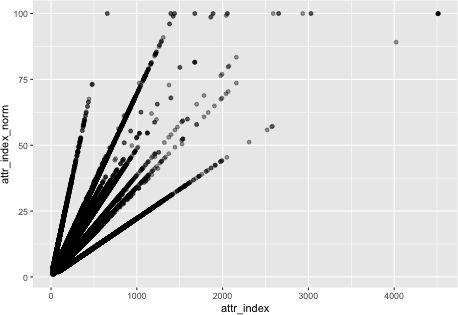
\includegraphics{Project_files/figure-latex/unnamed-chunk-8-1.png}

\begin{Shaded}
\begin{Highlighting}[]
\FunctionTok{ggplot}\NormalTok{() }\SpecialCharTok{+} \FunctionTok{geom\_point}\NormalTok{(}\AttributeTok{data =}\NormalTok{ my\_data, }\FunctionTok{aes}\NormalTok{(}\AttributeTok{x =}\NormalTok{ attr\_index, }\AttributeTok{y =}\NormalTok{ attr\_index\_norm),}
    \AttributeTok{alpha =} \FloatTok{0.4}\NormalTok{) }\SpecialCharTok{+} \FunctionTok{facet\_wrap}\NormalTok{(}\SpecialCharTok{\textasciitilde{}}\NormalTok{city\_day)}
\end{Highlighting}
\end{Shaded}

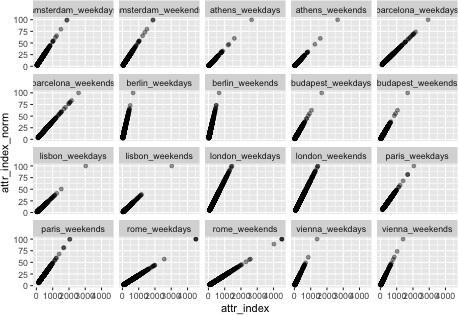
\includegraphics{Project_files/figure-latex/unnamed-chunk-8-2.png}

attr\_index and attr\_index\_norm are same, attr\_index\_norm is just
normalized attr\_index

\begin{Shaded}
\begin{Highlighting}[]
\FunctionTok{ggplot}\NormalTok{() }\SpecialCharTok{+} \FunctionTok{geom\_point}\NormalTok{(}\AttributeTok{data =}\NormalTok{ my\_data, }\FunctionTok{aes}\NormalTok{(}\AttributeTok{x =}\NormalTok{ rest\_index, }\AttributeTok{y =}\NormalTok{ rest\_index\_norm),}
    \AttributeTok{alpha =} \FloatTok{0.4}\NormalTok{)}
\end{Highlighting}
\end{Shaded}

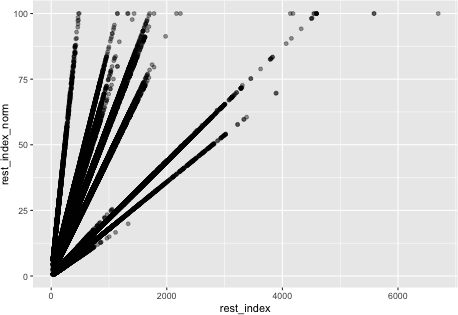
\includegraphics{Project_files/figure-latex/unnamed-chunk-9-1.png}

\begin{Shaded}
\begin{Highlighting}[]
\FunctionTok{ggplot}\NormalTok{() }\SpecialCharTok{+} \FunctionTok{geom\_point}\NormalTok{(}\AttributeTok{data =}\NormalTok{ my\_data, }\FunctionTok{aes}\NormalTok{(}\AttributeTok{x =}\NormalTok{ rest\_index, }\AttributeTok{y =}\NormalTok{ rest\_index\_norm),}
    \AttributeTok{alpha =} \FloatTok{0.4}\NormalTok{) }\SpecialCharTok{+} \FunctionTok{facet\_wrap}\NormalTok{(}\SpecialCharTok{\textasciitilde{}}\NormalTok{city\_day)}
\end{Highlighting}
\end{Shaded}

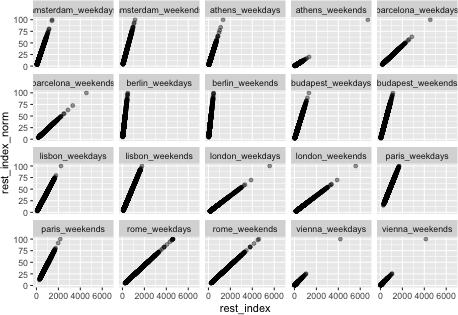
\includegraphics{Project_files/figure-latex/unnamed-chunk-9-2.png}

rest\_index and rest\_index\_norm are same, rest\_index\_norm is just
normalized rest\_index.

removing attr\_index and rest\_index

\begin{Shaded}
\begin{Highlighting}[]
\NormalTok{my\_data }\OtherTok{=} \FunctionTok{select}\NormalTok{(my\_data, }\SpecialCharTok{{-}}\FunctionTok{c}\NormalTok{(attr\_index, rest\_index))}
\FunctionTok{head}\NormalTok{(my\_data)}
\end{Highlighting}
\end{Shaded}

\begin{verbatim}
##   X  realSum    room_type person_capacity host_is_superhost multi biz
## 1 0 194.0337 Private room               2             False     1   0
## 2 1 344.2458 Private room               4             False     0   0
## 3 2 264.1014 Private room               2             False     0   1
## 4 3 433.5294 Private room               4             False     0   1
## 5 4 485.5529 Private room               2              True     0   0
## 6 5 552.8086 Private room               3             False     0   0
##   cleanliness_rating guest_satisfaction_overall bedrooms      dist metro_dist
## 1                 10                         93        1 5.0229638  2.5393800
## 2                  8                         85        1 0.4883893  0.2394039
## 3                  9                         87        1 5.7483119  3.6516213
## 4                  9                         90        2 0.3848620  0.4398761
## 5                 10                         98        1 0.5447382  0.3186926
## 6                  8                        100        2 2.1314201  1.9046682
##   attr_index_norm rest_index_norm     lng      lat           city_day
## 1        4.166708        6.846473 4.90569 52.41772 amsterdam_weekdays
## 2       33.421209       58.342928 4.90005 52.37432 amsterdam_weekdays
## 3        3.985908        6.646700 4.97512 52.36103 amsterdam_weekdays
## 4       26.119108       60.973565 4.89417 52.37663 amsterdam_weekdays
## 5       29.272733       56.811677 4.90051 52.37508 amsterdam_weekdays
## 6        9.255191       15.692376 4.87699 52.38966 amsterdam_weekdays
\end{verbatim}

\hypertarget{outliers-using-iqr-range}{%
\subsection{Outliers using IQR Range}\label{outliers-using-iqr-range}}

\hypertarget{filtering-out-the-outliers-from-data-out-of-iqr-ranges}{%
\subsubsection{Filtering out the Outliers from Data Out of IQR
Ranges}\label{filtering-out-the-outliers-from-data-out-of-iqr-ranges}}

\begin{Shaded}
\begin{Highlighting}[]
\CommentTok{\# Initialize an empty list to store the outliers}
\NormalTok{outliers\_list }\OtherTok{\textless{}{-}} \FunctionTok{list}\NormalTok{()}

\CommentTok{\# Initialize an empty list to store the filtered data}
\CommentTok{\# frames}
\NormalTok{df\_list\_filtered }\OtherTok{\textless{}{-}} \FunctionTok{list}\NormalTok{()}

\CommentTok{\# Loop through each file and read it into a data frame}
\CommentTok{\# after removing outliers}
\ControlFlowTok{for}\NormalTok{ (i }\ControlFlowTok{in} \FunctionTok{seq\_along}\NormalTok{(file\_list)) \{}
\NormalTok{    df\_filtered }\OtherTok{\textless{}{-}} \FunctionTok{read.csv}\NormalTok{(file\_list[i])}

    \CommentTok{\# Add a new column with the city\_day}
\NormalTok{    df\_filtered}\SpecialCharTok{$}\NormalTok{city\_day }\OtherTok{\textless{}{-}} \FunctionTok{gsub}\NormalTok{(}\StringTok{"}\SpecialCharTok{\textbackslash{}\textbackslash{}}\StringTok{.csv"}\NormalTok{, }\StringTok{""}\NormalTok{, }\FunctionTok{basename}\NormalTok{(file\_list[i]))}

\NormalTok{    iqr\_var1 }\OtherTok{\textless{}{-}} \FunctionTok{IQR}\NormalTok{(df\_filtered}\SpecialCharTok{$}\NormalTok{realSum)}

    \CommentTok{\# Calculate the upper and lower bounds for each}
    \CommentTok{\# variable}
\NormalTok{    upper\_var1 }\OtherTok{\textless{}{-}} \FunctionTok{quantile}\NormalTok{(df\_filtered}\SpecialCharTok{$}\NormalTok{realSum, }\FloatTok{0.75}\NormalTok{) }\SpecialCharTok{+} \FloatTok{1.5} \SpecialCharTok{*}
\NormalTok{        iqr\_var1}
\NormalTok{    lower\_var1 }\OtherTok{\textless{}{-}} \FunctionTok{quantile}\NormalTok{(df\_filtered}\SpecialCharTok{$}\NormalTok{realSum, }\FloatTok{0.25}\NormalTok{) }\SpecialCharTok{{-}} \FloatTok{1.5} \SpecialCharTok{*}
\NormalTok{        iqr\_var1}

    \CommentTok{\# Filter the data based on the upper and lower bounds}
    \CommentTok{\# for each variable}
\NormalTok{    filtered\_data }\OtherTok{\textless{}{-}} \FunctionTok{filter}\NormalTok{(df\_filtered, realSum }\SpecialCharTok{\textgreater{}}\NormalTok{ lower\_var1 }\SpecialCharTok{\&}
\NormalTok{        realSum }\SpecialCharTok{\textless{}}\NormalTok{ upper\_var1)}

    \CommentTok{\# Append the filtered data frame to the list}
\NormalTok{    df\_list\_filtered[[i]] }\OtherTok{\textless{}{-}}\NormalTok{ filtered\_data}

    \CommentTok{\# Get the rows that were removed while filtering}
\NormalTok{    outliers }\OtherTok{\textless{}{-}} \FunctionTok{anti\_join}\NormalTok{(df\_filtered, filtered\_data)}

    \CommentTok{\# Append the outliers to the list}
\NormalTok{    outliers\_list[[i]] }\OtherTok{\textless{}{-}}\NormalTok{ outliers}
\NormalTok{\}}


\CommentTok{\# Combine all the filtered data frames into a single}
\CommentTok{\# dataset}
\NormalTok{my\_data\_filtered }\OtherTok{\textless{}{-}} \FunctionTok{bind\_rows}\NormalTok{(df\_list\_filtered)}

\CommentTok{\# Removing the .csv ext}
\NormalTok{my\_data\_filtered}\SpecialCharTok{$}\NormalTok{city\_day }\OtherTok{\textless{}{-}} \FunctionTok{gsub}\NormalTok{(}\StringTok{"}\SpecialCharTok{\textbackslash{}\textbackslash{}}\StringTok{.csv"}\NormalTok{, }\StringTok{""}\NormalTok{, my\_data\_filtered}\SpecialCharTok{$}\NormalTok{city\_day)}

\FunctionTok{summary}\NormalTok{(my\_data\_filtered)}
\end{Highlighting}
\end{Shaded}

\begin{verbatim}
##        X           realSum         room_type         room_shared       
##  Min.   :   0   Min.   :  34.78   Length:48970       Length:48970      
##  1st Qu.: 645   1st Qu.: 145.23   Class :character   Class :character  
##  Median :1340   Median : 204.27   Mode  :character   Mode  :character  
##  Mean   :1621   Mean   : 244.35                                        
##  3rd Qu.:2385   3rd Qu.: 295.27                                        
##  Max.   :5378   Max.   :1229.11                                        
##  room_private       person_capacity host_is_superhost      multi       
##  Length:48970       Min.   :2.00    Length:48970       Min.   :0.0000  
##  Class :character   1st Qu.:2.00    Class :character   1st Qu.:0.0000  
##  Mode  :character   Median :3.00    Mode  :character   Median :0.0000  
##                     Mean   :3.08                       Mean   :0.2953  
##                     3rd Qu.:4.00                       3rd Qu.:1.0000  
##                     Max.   :6.00                       Max.   :1.0000  
##       biz        cleanliness_rating guest_satisfaction_overall    bedrooms     
##  Min.   :0.000   Min.   : 2.000     Min.   : 20.00             Min.   : 0.000  
##  1st Qu.:0.000   1st Qu.: 9.000     1st Qu.: 90.00             1st Qu.: 1.000  
##  Median :0.000   Median :10.000     Median : 95.00             Median : 1.000  
##  Mean   :0.342   Mean   : 9.384     Mean   : 92.57             Mean   : 1.118  
##  3rd Qu.:1.000   3rd Qu.:10.000     3rd Qu.: 98.00             3rd Qu.: 1.000  
##  Max.   :1.000   Max.   :10.000     Max.   :100.00             Max.   :10.000  
##       dist            metro_dist          attr_index      attr_index_norm   
##  Min.   : 0.01506   Min.   : 0.002301   Min.   :  15.15   Min.   :  0.9263  
##  1st Qu.: 1.48598   1st Qu.: 0.250718   1st Qu.: 133.75   1st Qu.:  6.2341  
##  Median : 2.66962   Median : 0.416955   Median : 228.54   Median : 11.1929  
##  Mean   : 3.24072   Mean   : 0.691774   Mean   : 285.15   Mean   : 13.0064  
##  3rd Qu.: 4.31533   3rd Qu.: 0.749700   3rd Qu.: 374.37   3rd Qu.: 16.9444  
##  Max.   :25.28456   Max.   :14.273577   Max.   :4513.56   Max.   :100.0000  
##    rest_index      rest_index_norm         lng                lat       
##  Min.   :  19.58   Min.   :  0.5928   Min.   :-9.22634   Min.   :37.95  
##  1st Qu.: 245.42   1st Qu.:  8.5601   1st Qu.:-0.07277   1st Qu.:41.40  
##  Median : 512.42   Median : 17.1799   Median : 4.87234   Median :47.51  
##  Mean   : 611.32   Mean   : 22.2861   Mean   : 7.40027   Mean   :45.66  
##  3rd Qu.: 818.44   3rd Qu.: 32.0321   3rd Qu.:13.52350   3rd Qu.:51.47  
##  Max.   :6696.16   Max.   :100.0000   Max.   :23.78602   Max.   :52.64  
##    city_day        
##  Length:48970      
##  Class :character  
##  Mode  :character  
##                    
##                    
## 
\end{verbatim}

\begin{Shaded}
\begin{Highlighting}[]
\CommentTok{\# Combine all the outliers into a single dataset}
\NormalTok{my\_outliers }\OtherTok{\textless{}{-}} \FunctionTok{bind\_rows}\NormalTok{(outliers\_list)}

\CommentTok{\# Removing the .csv ext}
\NormalTok{my\_outliers}\SpecialCharTok{$}\NormalTok{city\_day }\OtherTok{\textless{}{-}} \FunctionTok{gsub}\NormalTok{(}\StringTok{"}\SpecialCharTok{\textbackslash{}\textbackslash{}}\StringTok{.csv"}\NormalTok{, }\StringTok{""}\NormalTok{, my\_outliers}\SpecialCharTok{$}\NormalTok{city\_day)}

\FunctionTok{summary}\NormalTok{(my\_outliers)}
\end{Highlighting}
\end{Shaded}

\begin{verbatim}
##        X           realSum         room_type         room_shared       
##  Min.   :   0   Min.   :  279.4   Length:2737        Length:2737       
##  1st Qu.: 666   1st Qu.:  469.2   Class :character   Class :character  
##  Median :1237   Median :  691.9   Mode  :character   Mode  :character  
##  Mean   :1614   Mean   :  915.5                                        
##  3rd Qu.:2310   3rd Qu.:  996.3                                        
##  Max.   :5374   Max.   :18545.5                                        
##  room_private       person_capacity host_is_superhost      multi      
##  Length:2737        Min.   :2.000   Length:2737        Min.   :0.000  
##  Class :character   1st Qu.:4.000   Class :character   1st Qu.:0.000  
##  Mode  :character   Median :5.000   Mode  :character   Median :0.000  
##                     Mean   :4.628                      Mean   :0.221  
##                     3rd Qu.:6.000                      3rd Qu.:0.000  
##                     Max.   :6.000                      Max.   :1.000  
##       biz         cleanliness_rating guest_satisfaction_overall    bedrooms    
##  Min.   :0.0000   Min.   : 2.000     Min.   : 20.00             Min.   :0.000  
##  1st Qu.:0.0000   1st Qu.: 9.000     1st Qu.: 91.00             1st Qu.:1.000  
##  Median :0.0000   Median :10.000     Median : 97.00             Median :2.000  
##  Mean   :0.4965   Mean   : 9.509     Mean   : 93.65             Mean   :1.886  
##  3rd Qu.:1.0000   3rd Qu.:10.000     3rd Qu.:100.00             3rd Qu.:2.000  
##  Max.   :1.0000   Max.   :10.000     Max.   :100.00             Max.   :6.000  
##       dist            metro_dist         attr_index     attr_index_norm  
##  Min.   : 0.01504   Min.   :0.006171   Min.   :  20.5   Min.   :  1.468  
##  1st Qu.: 1.04119   1st Qu.:0.218081   1st Qu.: 225.1   1st Qu.: 11.719  
##  Median : 1.89579   Median :0.352339   Median : 385.0   Median : 17.958  
##  Mean   : 2.30674   Mean   :0.498426   Mean   : 456.2   Mean   : 20.892  
##  3rd Qu.: 3.00820   3rd Qu.:0.576430   3rd Qu.: 610.6   3rd Qu.: 25.953  
##  Max.   :21.29515   Max.   :8.918036   Max.   :2040.4   Max.   :100.000  
##    rest_index     rest_index_norm        lng                lat       
##  Min.   :  27.9   Min.   :  0.667   Min.   :-9.22476   Min.   :37.96  
##  1st Qu.: 408.5   1st Qu.: 14.187   1st Qu.:-0.06677   1st Qu.:41.41  
##  Median : 739.9   Median : 30.001   Median : 4.88384   Median :47.51  
##  Mean   : 904.9   Mean   : 31.734   Mean   : 7.88764   Mean   :45.93  
##  3rd Qu.:1269.7   3rd Qu.: 45.426   3rd Qu.:13.44666   3rd Qu.:51.50  
##  Max.   :4183.1   Max.   :100.000   Max.   :23.75400   Max.   :52.58  
##    city_day        
##  Length:2737       
##  Class :character  
##  Mode  :character  
##                    
##                    
## 
\end{verbatim}

\hypertarget{percentage-of-outliers-outside-of-iqr-range.}{%
\subsubsection{Percentage of Outliers outside of IQR
range.}\label{percentage-of-outliers-outside-of-iqr-range.}}

\begin{Shaded}
\begin{Highlighting}[]
\CommentTok{\# Create empty table}
\NormalTok{outliers\_table }\OtherTok{\textless{}{-}} \FunctionTok{data.frame}\NormalTok{(}\AttributeTok{City\_day =} \FunctionTok{character}\NormalTok{(), }\AttributeTok{Data\_Length =} \FunctionTok{numeric}\NormalTok{(),}
    \AttributeTok{Percent\_Outliers =} \FunctionTok{numeric}\NormalTok{(), }\AttributeTok{stringsAsFactors =} \ConstantTok{FALSE}\NormalTok{)}

\CommentTok{\# Loop through city\_data and fill in table}
\ControlFlowTok{for}\NormalTok{ (city\_day }\ControlFlowTok{in} \FunctionTok{unique}\NormalTok{(my\_data}\SpecialCharTok{$}\NormalTok{city\_day)) \{}
\NormalTok{    x }\OtherTok{=}\NormalTok{ my\_data[my\_data}\SpecialCharTok{$}\NormalTok{city\_day }\SpecialCharTok{==}\NormalTok{ city\_day, ]}\SpecialCharTok{$}\NormalTok{realSum}
\NormalTok{    q1 }\OtherTok{\textless{}{-}} \FunctionTok{quantile}\NormalTok{(x, }\FloatTok{0.25}\NormalTok{)}
\NormalTok{    q3 }\OtherTok{\textless{}{-}} \FunctionTok{quantile}\NormalTok{(x, }\FloatTok{0.75}\NormalTok{)}
\NormalTok{    iqr }\OtherTok{\textless{}{-}} \FunctionTok{IQR}\NormalTok{(x)}
\NormalTok{    upper\_bound }\OtherTok{\textless{}{-}}\NormalTok{ q3 }\SpecialCharTok{+} \FloatTok{1.5} \SpecialCharTok{*}\NormalTok{ iqr}
\NormalTok{    lower\_bound }\OtherTok{\textless{}{-}}\NormalTok{ q1 }\SpecialCharTok{{-}} \FloatTok{1.5} \SpecialCharTok{*}\NormalTok{ iqr}
\NormalTok{    x\_no\_outliers }\OtherTok{\textless{}{-}}\NormalTok{ x[x }\SpecialCharTok{\textgreater{}=}\NormalTok{ lower\_bound }\SpecialCharTok{\&}\NormalTok{ x }\SpecialCharTok{\textless{}=}\NormalTok{ upper\_bound]}
\NormalTok{    percent\_outliers }\OtherTok{\textless{}{-}}\NormalTok{ ((}\FunctionTok{length}\NormalTok{(x) }\SpecialCharTok{{-}} \FunctionTok{length}\NormalTok{(x\_no\_outliers))}\SpecialCharTok{/}\FunctionTok{length}\NormalTok{(x)) }\SpecialCharTok{*}
        \DecValTok{100}

    \CommentTok{\# Add row to table}
\NormalTok{    outliers\_table }\OtherTok{\textless{}{-}} \FunctionTok{rbind}\NormalTok{(outliers\_table, }\FunctionTok{data.frame}\NormalTok{(}\AttributeTok{City\_day =}\NormalTok{ city\_day,}
        \AttributeTok{Data\_Length =} \FunctionTok{length}\NormalTok{(x), }\AttributeTok{Percent\_Outliers =}\NormalTok{ percent\_outliers))}
\NormalTok{\}}

\CommentTok{\# Format table using kable}
\FunctionTok{kable}\NormalTok{(outliers\_table, }\AttributeTok{format =} \StringTok{"markdown"}\NormalTok{)}
\end{Highlighting}
\end{Shaded}

\begin{longtable}[]{@{}lrr@{}}
\toprule()
City\_day & Data\_Length & Percent\_Outliers \\
\midrule()
\endhead
amsterdam\_weekdays & 1103 & 5.077063 \\
amsterdam\_weekends & 977 & 5.629478 \\
athens\_weekdays & 2653 & 5.767056 \\
athens\_weekends & 2627 & 5.405405 \\
barcelona\_weekdays & 1555 & 7.524116 \\
barcelona\_weekends & 1278 & 8.059468 \\
berlin\_weekdays & 1284 & 6.308411 \\
berlin\_weekends & 1200 & 6.166667 \\
budapest\_weekdays & 2074 & 5.930569 \\
budapest\_weekends & 1948 & 5.544148 \\
lisbon\_weekdays & 2857 & 3.360168 \\
lisbon\_weekends & 2906 & 3.475568 \\
london\_weekdays & 4614 & 5.353273 \\
london\_weekends & 5379 & 5.521472 \\
paris\_weekdays & 3130 & 6.134185 \\
paris\_weekends & 3558 & 5.368184 \\
rome\_weekdays & 4492 & 5.031167 \\
rome\_weekends & 4535 & 5.005513 \\
vienna\_weekdays & 1738 & 4.257767 \\
vienna\_weekends & 1799 & 4.113396 \\
\bottomrule()
\end{longtable}

\hypertarget{spilt-training-and-testing-data}{%
\subsection{Spilt Training and Testing
Data}\label{spilt-training-and-testing-data}}

\begin{Shaded}
\begin{Highlighting}[]
\FunctionTok{set.seed}\NormalTok{(}\DecValTok{123456789}\NormalTok{)}
\NormalTok{my\_data\_train }\OtherTok{\textless{}{-}}\NormalTok{ my\_data[}\FunctionTok{sample}\NormalTok{(}\FunctionTok{nrow}\NormalTok{(my\_data), }\FloatTok{0.7} \SpecialCharTok{*} \FunctionTok{nrow}\NormalTok{(my\_data)),}
\NormalTok{    ]}
\NormalTok{my\_data\_test }\OtherTok{\textless{}{-}}\NormalTok{ my\_data[}\FunctionTok{setdiff}\NormalTok{(}\DecValTok{1}\SpecialCharTok{:}\FunctionTok{nrow}\NormalTok{(my\_data), }\FunctionTok{rownames}\NormalTok{(my\_data\_train)),}
\NormalTok{    ]}
\FunctionTok{dim}\NormalTok{(my\_data\_train)}
\end{Highlighting}
\end{Shaded}

\begin{verbatim}
## [1] 36194    17
\end{verbatim}

\begin{Shaded}
\begin{Highlighting}[]
\FunctionTok{dim}\NormalTok{(my\_data\_test)}
\end{Highlighting}
\end{Shaded}

\begin{verbatim}
## [1] 15513    17
\end{verbatim}

\hypertarget{exploratory-data-analysis}{%
\section{Exploratory Data Analysis}\label{exploratory-data-analysis}}

\hypertarget{outlier-analysis}{%
\subsection{Outlier Analysis}\label{outlier-analysis}}

\hypertarget{metro-dist-vs-real-sum}{%
\subsubsection{Metro Dist vs Real Sum}\label{metro-dist-vs-real-sum}}

We have planned to analyse the filtered data along with outlier data.
Here outlier data represents the hotel rooms with high prices.

\begin{Shaded}
\begin{Highlighting}[]
\FunctionTok{ggplot}\NormalTok{() }\SpecialCharTok{+} \FunctionTok{geom\_point}\NormalTok{(}\AttributeTok{data =}\NormalTok{ my\_data\_filtered, }\FunctionTok{aes}\NormalTok{(}\AttributeTok{x =}\NormalTok{ realSum,}
    \AttributeTok{y =}\NormalTok{ metro\_dist, }\AttributeTok{color =} \StringTok{"Filtered Data"}\NormalTok{), }\AttributeTok{alpha =} \FloatTok{0.4}\NormalTok{) }\SpecialCharTok{+}
    \FunctionTok{geom\_point}\NormalTok{(}\AttributeTok{data =}\NormalTok{ my\_outliers, }\FunctionTok{aes}\NormalTok{(}\AttributeTok{x =}\NormalTok{ realSum, }\AttributeTok{y =}\NormalTok{ metro\_dist,}
        \AttributeTok{color =} \StringTok{"Outliers"}\NormalTok{), }\AttributeTok{alpha =} \FloatTok{0.4}\NormalTok{) }\SpecialCharTok{+} \FunctionTok{scale\_color\_manual}\NormalTok{(}\AttributeTok{values =} \FunctionTok{c}\NormalTok{(}\StringTok{\textasciigrave{}}\AttributeTok{Filtered Data}\StringTok{\textasciigrave{}} \OtherTok{=} \StringTok{"blue"}\NormalTok{,}
    \AttributeTok{Outliers =} \StringTok{"red"}\NormalTok{))}
\end{Highlighting}
\end{Shaded}

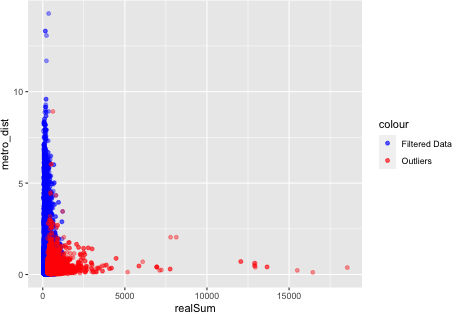
\includegraphics{Project_files/figure-latex/unnamed-chunk-14-1.png}

\begin{Shaded}
\begin{Highlighting}[]
\FunctionTok{ggplot}\NormalTok{() }\SpecialCharTok{+} \FunctionTok{geom\_point}\NormalTok{(}\AttributeTok{data =}\NormalTok{ my\_data\_filtered, }\FunctionTok{aes}\NormalTok{(}\AttributeTok{x =}\NormalTok{ realSum,}
    \AttributeTok{y =}\NormalTok{ metro\_dist, }\AttributeTok{color =} \StringTok{"Filtered Data"}\NormalTok{), }\AttributeTok{alpha =} \FloatTok{0.4}\NormalTok{) }\SpecialCharTok{+}
    \FunctionTok{geom\_point}\NormalTok{(}\AttributeTok{data =}\NormalTok{ my\_outliers, }\FunctionTok{aes}\NormalTok{(}\AttributeTok{x =}\NormalTok{ realSum, }\AttributeTok{y =}\NormalTok{ metro\_dist,}
        \AttributeTok{color =} \StringTok{"Outliers"}\NormalTok{), }\AttributeTok{alpha =} \FloatTok{0.4}\NormalTok{) }\SpecialCharTok{+} \FunctionTok{scale\_color\_manual}\NormalTok{(}\AttributeTok{values =} \FunctionTok{c}\NormalTok{(}\StringTok{\textasciigrave{}}\AttributeTok{Filtered Data}\StringTok{\textasciigrave{}} \OtherTok{=} \StringTok{"blue"}\NormalTok{,}
    \AttributeTok{Outliers =} \StringTok{"red"}\NormalTok{)) }\SpecialCharTok{+} \FunctionTok{facet\_wrap}\NormalTok{(}\SpecialCharTok{\textasciitilde{}}\NormalTok{city\_day)}
\end{Highlighting}
\end{Shaded}

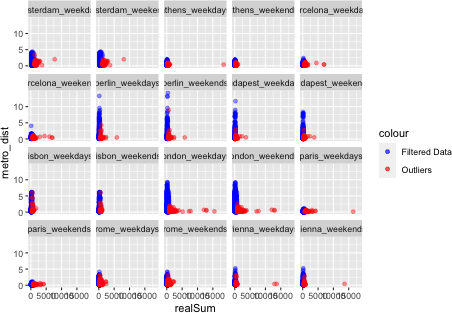
\includegraphics{Project_files/figure-latex/unnamed-chunk-14-2.png} In
general the rooms that are closer to metro have comparatively higher
prices. But, in Rome city the distance to metro is almost same for both
categories of price.

\hypertarget{real-sum-vs-distance}{%
\subsubsection{Real Sum vs Distance}\label{real-sum-vs-distance}}

\begin{Shaded}
\begin{Highlighting}[]
\FunctionTok{ggplot}\NormalTok{() }\SpecialCharTok{+} \FunctionTok{geom\_point}\NormalTok{(}\AttributeTok{data =}\NormalTok{ my\_data\_filtered, }\FunctionTok{aes}\NormalTok{(}\AttributeTok{x =}\NormalTok{ realSum,}
    \AttributeTok{y =}\NormalTok{ dist, }\AttributeTok{color =} \StringTok{"Filtered Data"}\NormalTok{), }\AttributeTok{alpha =} \FloatTok{0.4}\NormalTok{) }\SpecialCharTok{+} \FunctionTok{geom\_point}\NormalTok{(}\AttributeTok{data =}\NormalTok{ my\_outliers,}
    \FunctionTok{aes}\NormalTok{(}\AttributeTok{x =}\NormalTok{ realSum, }\AttributeTok{y =}\NormalTok{ dist, }\AttributeTok{color =} \StringTok{"Outliers"}\NormalTok{), }\AttributeTok{alpha =} \FloatTok{0.4}\NormalTok{) }\SpecialCharTok{+}
    \FunctionTok{scale\_color\_manual}\NormalTok{(}\AttributeTok{values =} \FunctionTok{c}\NormalTok{(}\StringTok{\textasciigrave{}}\AttributeTok{Filtered Data}\StringTok{\textasciigrave{}} \OtherTok{=} \StringTok{"blue"}\NormalTok{, }\AttributeTok{Outliers =} \StringTok{"red"}\NormalTok{))}
\end{Highlighting}
\end{Shaded}

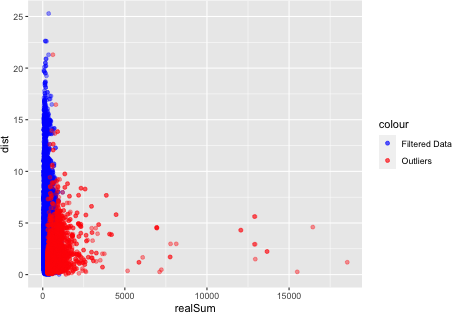
\includegraphics{Project_files/figure-latex/unnamed-chunk-15-1.png}

\begin{Shaded}
\begin{Highlighting}[]
\FunctionTok{ggplot}\NormalTok{() }\SpecialCharTok{+} \FunctionTok{geom\_point}\NormalTok{(}\AttributeTok{data =}\NormalTok{ my\_data\_filtered, }\FunctionTok{aes}\NormalTok{(}\AttributeTok{x =}\NormalTok{ realSum,}
    \AttributeTok{y =}\NormalTok{ dist, }\AttributeTok{color =} \StringTok{"Filtered Data"}\NormalTok{), }\AttributeTok{alpha =} \FloatTok{0.4}\NormalTok{) }\SpecialCharTok{+} \FunctionTok{geom\_point}\NormalTok{(}\AttributeTok{data =}\NormalTok{ my\_outliers,}
    \FunctionTok{aes}\NormalTok{(}\AttributeTok{x =}\NormalTok{ realSum, }\AttributeTok{y =}\NormalTok{ dist, }\AttributeTok{color =} \StringTok{"Outliers"}\NormalTok{), }\AttributeTok{alpha =} \FloatTok{0.4}\NormalTok{) }\SpecialCharTok{+}
    \FunctionTok{scale\_color\_manual}\NormalTok{(}\AttributeTok{values =} \FunctionTok{c}\NormalTok{(}\StringTok{\textasciigrave{}}\AttributeTok{Filtered Data}\StringTok{\textasciigrave{}} \OtherTok{=} \StringTok{"blue"}\NormalTok{, }\AttributeTok{Outliers =} \StringTok{"red"}\NormalTok{)) }\SpecialCharTok{+}
    \FunctionTok{facet\_wrap}\NormalTok{(}\SpecialCharTok{\textasciitilde{}}\NormalTok{city\_day)}
\end{Highlighting}
\end{Shaded}

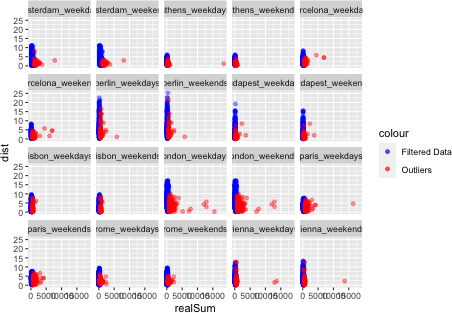
\includegraphics{Project_files/figure-latex/unnamed-chunk-15-2.png} In
general the pricey rooms are near to the centre of the city.

\hypertarget{real-sum-vs-attraction-index-normal}{%
\subsubsection{Real Sum vs Attraction Index
Normal}\label{real-sum-vs-attraction-index-normal}}

\begin{Shaded}
\begin{Highlighting}[]
\FunctionTok{ggplot}\NormalTok{() }\SpecialCharTok{+} \FunctionTok{geom\_point}\NormalTok{(}\AttributeTok{data =}\NormalTok{ my\_data\_filtered, }\FunctionTok{aes}\NormalTok{(}\AttributeTok{x =}\NormalTok{ realSum,}
    \AttributeTok{y =}\NormalTok{ attr\_index\_norm, }\AttributeTok{color =} \StringTok{"Filtered Data"}\NormalTok{), }\AttributeTok{alpha =} \FloatTok{0.4}\NormalTok{) }\SpecialCharTok{+}
    \FunctionTok{geom\_point}\NormalTok{(}\AttributeTok{data =}\NormalTok{ my\_outliers, }\FunctionTok{aes}\NormalTok{(}\AttributeTok{x =}\NormalTok{ realSum, }\AttributeTok{y =}\NormalTok{ attr\_index\_norm,}
        \AttributeTok{color =} \StringTok{"Outliers"}\NormalTok{), }\AttributeTok{alpha =} \FloatTok{0.4}\NormalTok{) }\SpecialCharTok{+} \FunctionTok{scale\_color\_manual}\NormalTok{(}\AttributeTok{values =} \FunctionTok{c}\NormalTok{(}\StringTok{\textasciigrave{}}\AttributeTok{Filtered Data}\StringTok{\textasciigrave{}} \OtherTok{=} \StringTok{"blue"}\NormalTok{,}
    \AttributeTok{Outliers =} \StringTok{"red"}\NormalTok{))}
\end{Highlighting}
\end{Shaded}

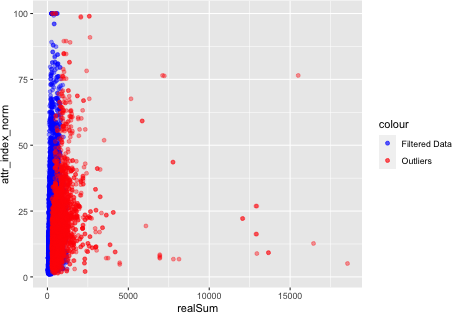
\includegraphics{Project_files/figure-latex/unnamed-chunk-16-1.png}

\begin{Shaded}
\begin{Highlighting}[]
\FunctionTok{ggplot}\NormalTok{() }\SpecialCharTok{+} \FunctionTok{geom\_point}\NormalTok{(}\AttributeTok{data =}\NormalTok{ my\_data\_filtered, }\FunctionTok{aes}\NormalTok{(}\AttributeTok{x =}\NormalTok{ realSum,}
    \AttributeTok{y =}\NormalTok{ attr\_index\_norm, }\AttributeTok{color =} \StringTok{"Filtered Data"}\NormalTok{), }\AttributeTok{alpha =} \FloatTok{0.4}\NormalTok{) }\SpecialCharTok{+}
    \FunctionTok{geom\_point}\NormalTok{(}\AttributeTok{data =}\NormalTok{ my\_outliers, }\FunctionTok{aes}\NormalTok{(}\AttributeTok{x =}\NormalTok{ realSum, }\AttributeTok{y =}\NormalTok{ attr\_index\_norm,}
        \AttributeTok{color =} \StringTok{"Outliers"}\NormalTok{), }\AttributeTok{alpha =} \FloatTok{0.4}\NormalTok{) }\SpecialCharTok{+} \FunctionTok{scale\_color\_manual}\NormalTok{(}\AttributeTok{values =} \FunctionTok{c}\NormalTok{(}\StringTok{\textasciigrave{}}\AttributeTok{Filtered Data}\StringTok{\textasciigrave{}} \OtherTok{=} \StringTok{"blue"}\NormalTok{,}
    \AttributeTok{Outliers =} \StringTok{"red"}\NormalTok{)) }\SpecialCharTok{+} \FunctionTok{facet\_wrap}\NormalTok{(}\SpecialCharTok{\textasciitilde{}}\NormalTok{city\_day)}
\end{Highlighting}
\end{Shaded}

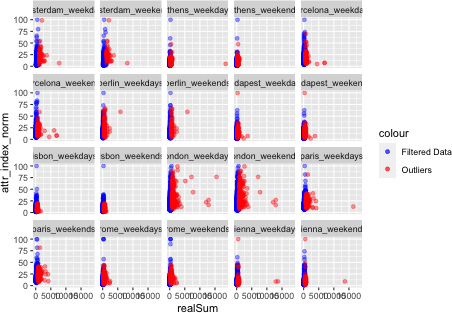
\includegraphics{Project_files/figure-latex/unnamed-chunk-16-2.png}

\begin{Shaded}
\begin{Highlighting}[]
\FunctionTok{ggplot}\NormalTok{() }\SpecialCharTok{+} \FunctionTok{geom\_point}\NormalTok{(}\AttributeTok{data =}\NormalTok{ my\_data\_filtered, }\FunctionTok{aes}\NormalTok{(}\AttributeTok{x =}\NormalTok{ realSum,}
    \AttributeTok{y =}\NormalTok{ attr\_index\_norm), }\AttributeTok{alpha =} \FloatTok{0.4}\NormalTok{) }\SpecialCharTok{+} \FunctionTok{geom\_point}\NormalTok{(}\AttributeTok{data =}\NormalTok{ my\_outliers,}
    \FunctionTok{aes}\NormalTok{(}\AttributeTok{x =}\NormalTok{ realSum, }\AttributeTok{y =}\NormalTok{ attr\_index\_norm), }\AttributeTok{alpha =} \FloatTok{0.4}\NormalTok{)}
\end{Highlighting}
\end{Shaded}

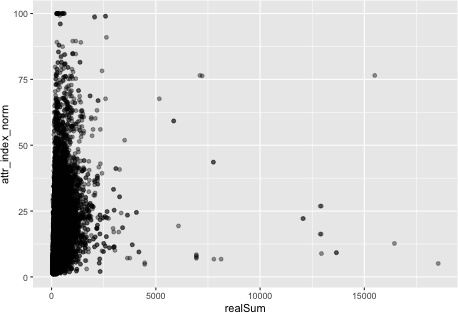
\includegraphics{Project_files/figure-latex/unnamed-chunk-16-3.png}

The range of values falling b/w outliers and normal data is almost same
. So there isn't a relationship b/w attr\_index and realSum.

\hypertarget{real-sum-vs-restaurant-index-normal}{%
\subsubsection{Real Sum vs Restaurant Index
Normal}\label{real-sum-vs-restaurant-index-normal}}

\begin{Shaded}
\begin{Highlighting}[]
\FunctionTok{ggplot}\NormalTok{() }\SpecialCharTok{+} \FunctionTok{geom\_point}\NormalTok{(}\AttributeTok{data =}\NormalTok{ my\_data\_filtered, }\FunctionTok{aes}\NormalTok{(}\AttributeTok{x =}\NormalTok{ realSum,}
    \AttributeTok{y =}\NormalTok{ rest\_index\_norm, }\AttributeTok{color =} \StringTok{"Filtered Data"}\NormalTok{), }\AttributeTok{alpha =} \FloatTok{0.4}\NormalTok{) }\SpecialCharTok{+}
    \FunctionTok{geom\_point}\NormalTok{(}\AttributeTok{data =}\NormalTok{ my\_outliers, }\FunctionTok{aes}\NormalTok{(}\AttributeTok{x =}\NormalTok{ realSum, }\AttributeTok{y =}\NormalTok{ rest\_index\_norm,}
        \AttributeTok{color =} \StringTok{"Outliers"}\NormalTok{), }\AttributeTok{alpha =} \FloatTok{0.4}\NormalTok{) }\SpecialCharTok{+} \FunctionTok{scale\_color\_manual}\NormalTok{(}\AttributeTok{values =} \FunctionTok{c}\NormalTok{(}\StringTok{\textasciigrave{}}\AttributeTok{Filtered Data}\StringTok{\textasciigrave{}} \OtherTok{=} \StringTok{"blue"}\NormalTok{,}
    \AttributeTok{Outliers =} \StringTok{"red"}\NormalTok{))}
\end{Highlighting}
\end{Shaded}

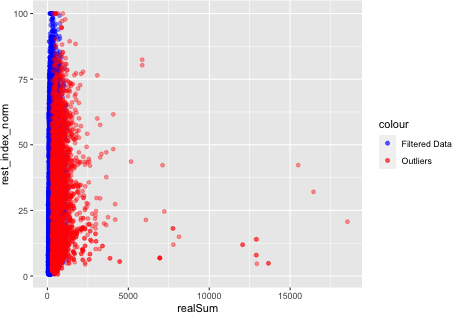
\includegraphics{Project_files/figure-latex/unnamed-chunk-17-1.png}

\begin{Shaded}
\begin{Highlighting}[]
\FunctionTok{ggplot}\NormalTok{() }\SpecialCharTok{+} \FunctionTok{geom\_point}\NormalTok{(}\AttributeTok{data =}\NormalTok{ my\_data\_filtered, }\FunctionTok{aes}\NormalTok{(}\AttributeTok{x =}\NormalTok{ realSum,}
    \AttributeTok{y =}\NormalTok{ rest\_index\_norm, }\AttributeTok{color =} \StringTok{"Filtered Data"}\NormalTok{), }\AttributeTok{alpha =} \FloatTok{0.4}\NormalTok{) }\SpecialCharTok{+}
    \FunctionTok{geom\_point}\NormalTok{(}\AttributeTok{data =}\NormalTok{ my\_outliers, }\FunctionTok{aes}\NormalTok{(}\AttributeTok{x =}\NormalTok{ realSum, }\AttributeTok{y =}\NormalTok{ rest\_index\_norm,}
        \AttributeTok{color =} \StringTok{"Outliers"}\NormalTok{), }\AttributeTok{alpha =} \FloatTok{0.4}\NormalTok{) }\SpecialCharTok{+} \FunctionTok{scale\_color\_manual}\NormalTok{(}\AttributeTok{values =} \FunctionTok{c}\NormalTok{(}\StringTok{\textasciigrave{}}\AttributeTok{Filtered Data}\StringTok{\textasciigrave{}} \OtherTok{=} \StringTok{"blue"}\NormalTok{,}
    \AttributeTok{Outliers =} \StringTok{"red"}\NormalTok{)) }\SpecialCharTok{+} \FunctionTok{facet\_wrap}\NormalTok{(}\SpecialCharTok{\textasciitilde{}}\NormalTok{city\_day)}
\end{Highlighting}
\end{Shaded}

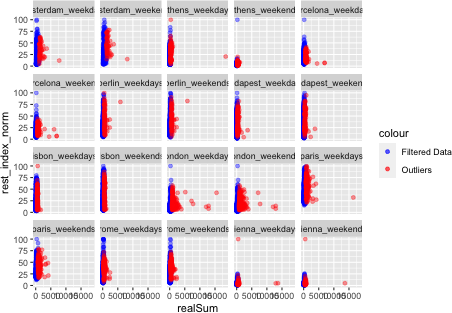
\includegraphics{Project_files/figure-latex/unnamed-chunk-17-2.png}

There is no relationship between outliers and rest\_index

\hypertarget{room-type-vs-real-sum}{%
\subsubsection{Room Type Vs Real Sum}\label{room-type-vs-real-sum}}

\begin{Shaded}
\begin{Highlighting}[]
\FunctionTok{ggplot}\NormalTok{(my\_data, }\FunctionTok{aes}\NormalTok{(}\AttributeTok{x =}\NormalTok{ realSum, }\AttributeTok{fill =}\NormalTok{ room\_type, }\AttributeTok{group =}\NormalTok{ room\_type)) }\SpecialCharTok{+}
    \FunctionTok{geom\_histogram}\NormalTok{(}\AttributeTok{alpha =} \FloatTok{0.5}\NormalTok{, }\AttributeTok{nbins =} \DecValTok{20}\NormalTok{) }\SpecialCharTok{+} \FunctionTok{theme}\NormalTok{(}\AttributeTok{axis.title.x =} \FunctionTok{element\_text}\NormalTok{(}\AttributeTok{size =} \DecValTok{14}\NormalTok{),}
    \AttributeTok{axis.title.y =} \FunctionTok{element\_text}\NormalTok{(}\AttributeTok{size =} \DecValTok{14}\NormalTok{))}
\end{Highlighting}
\end{Shaded}

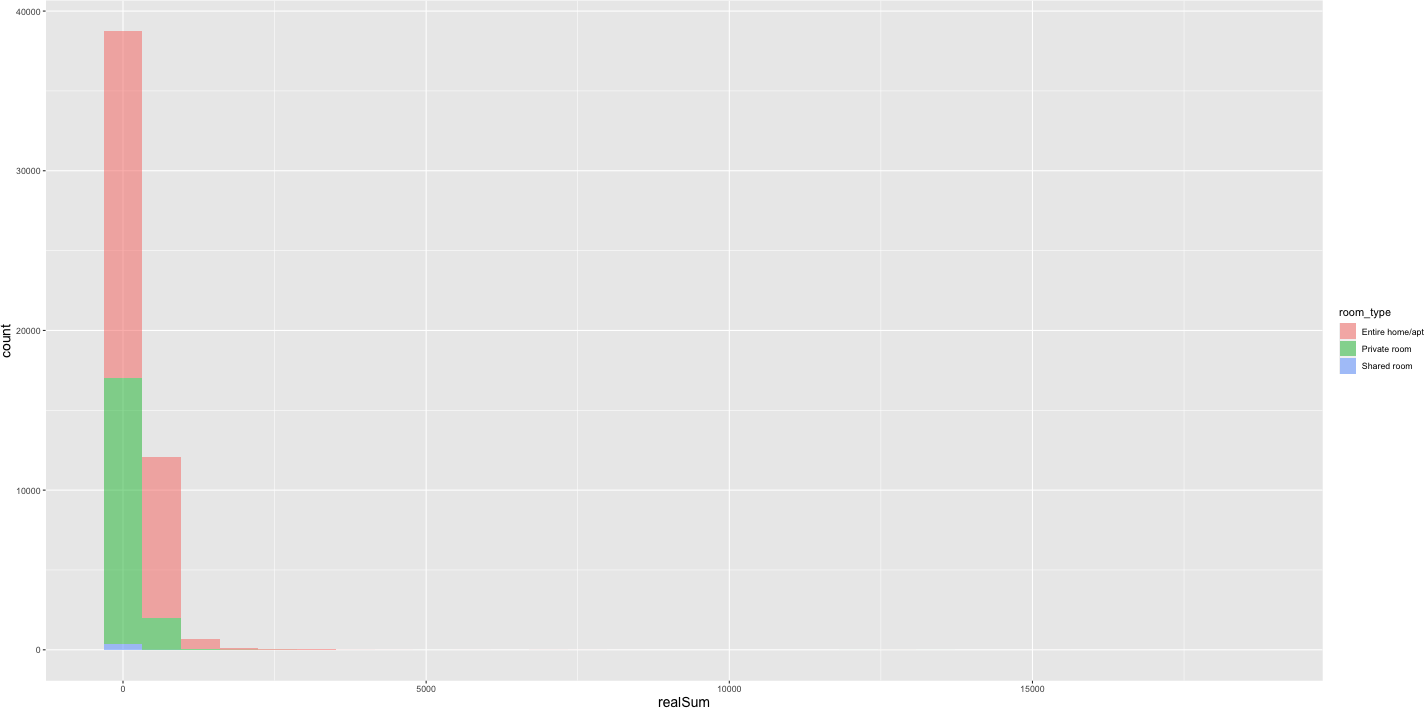
\includegraphics{Project_files/figure-latex/unnamed-chunk-18-1.png}

\begin{Shaded}
\begin{Highlighting}[]
\FunctionTok{ggplot}\NormalTok{(my\_data\_filtered, }\FunctionTok{aes}\NormalTok{(}\AttributeTok{x =}\NormalTok{ realSum, }\AttributeTok{fill =}\NormalTok{ room\_type, }\AttributeTok{group =}\NormalTok{ room\_type)) }\SpecialCharTok{+}
    \FunctionTok{geom\_histogram}\NormalTok{(}\AttributeTok{alpha =} \FloatTok{0.5}\NormalTok{, }\AttributeTok{nbins =} \DecValTok{20}\NormalTok{) }\SpecialCharTok{+} \FunctionTok{theme}\NormalTok{(}\AttributeTok{axis.title.x =} \FunctionTok{element\_text}\NormalTok{(}\AttributeTok{size =} \DecValTok{14}\NormalTok{),}
    \AttributeTok{axis.title.y =} \FunctionTok{element\_text}\NormalTok{(}\AttributeTok{size =} \DecValTok{14}\NormalTok{))}
\end{Highlighting}
\end{Shaded}

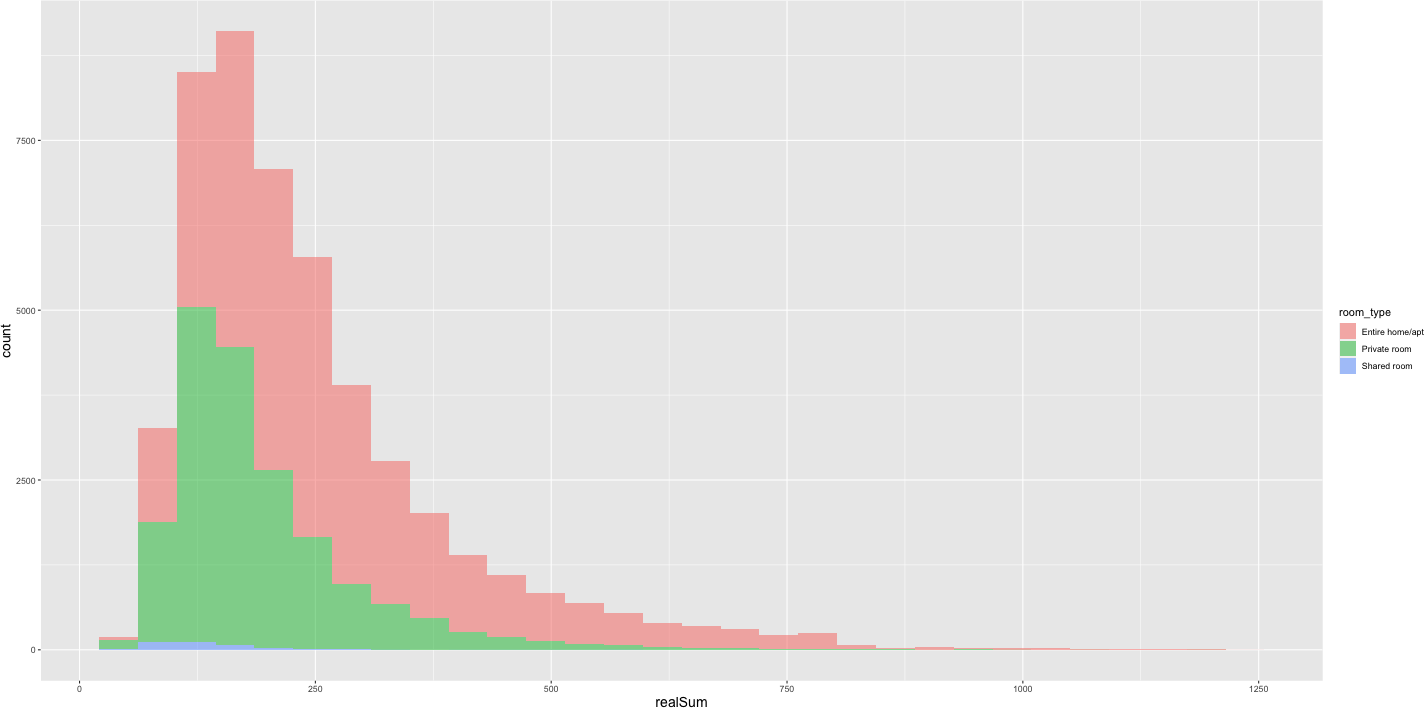
\includegraphics{Project_files/figure-latex/unnamed-chunk-18-2.png}

\begin{Shaded}
\begin{Highlighting}[]
\FunctionTok{ggplot}\NormalTok{(my\_data\_filtered, }\FunctionTok{aes}\NormalTok{(}\AttributeTok{x =}\NormalTok{ realSum, }\AttributeTok{fill =}\NormalTok{ room\_type, }\AttributeTok{group =}\NormalTok{ room\_type)) }\SpecialCharTok{+}
    \FunctionTok{geom\_histogram}\NormalTok{(}\AttributeTok{alpha =} \FloatTok{0.5}\NormalTok{, }\AttributeTok{nbins =} \DecValTok{20}\NormalTok{) }\SpecialCharTok{+} \FunctionTok{theme}\NormalTok{(}\AttributeTok{axis.title.x =} \FunctionTok{element\_text}\NormalTok{(}\AttributeTok{size =} \DecValTok{14}\NormalTok{),}
    \AttributeTok{axis.title.y =} \FunctionTok{element\_text}\NormalTok{(}\AttributeTok{size =} \DecValTok{14}\NormalTok{)) }\SpecialCharTok{+} \FunctionTok{facet\_wrap}\NormalTok{(}\SpecialCharTok{\textasciitilde{}}\NormalTok{city\_day)}
\end{Highlighting}
\end{Shaded}

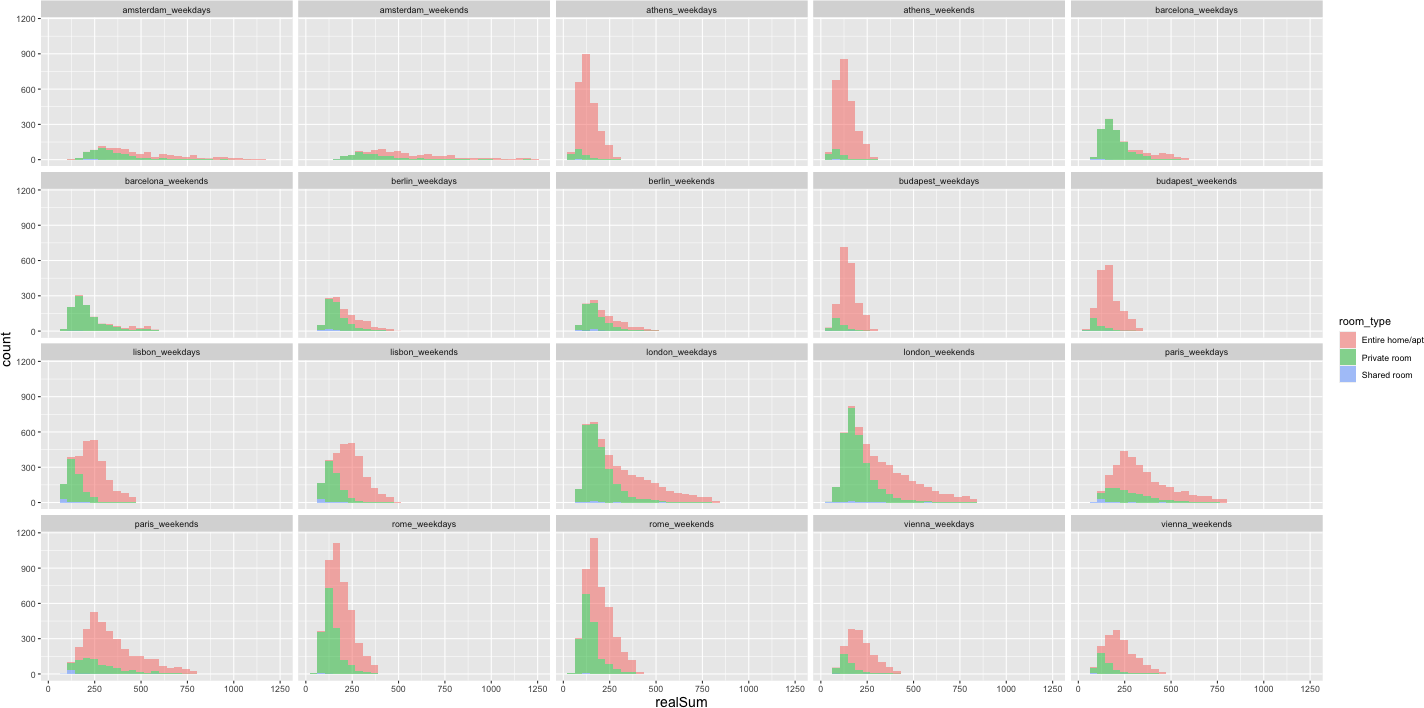
\includegraphics{Project_files/figure-latex/unnamed-chunk-18-3.png}

The price of entire home/apt tend to be higher compared to other two
categories. And the count of entire home /apt is also more.

\hypertarget{room-type-vs-person-capacity}{%
\subsubsection{Room Type Vs Person
Capacity}\label{room-type-vs-person-capacity}}

\begin{Shaded}
\begin{Highlighting}[]
\FunctionTok{ggplot}\NormalTok{(my\_data, }\FunctionTok{aes}\NormalTok{(}\AttributeTok{x =}\NormalTok{ realSum, }\AttributeTok{fill =}\NormalTok{ person\_capacity, }\AttributeTok{group =}\NormalTok{ person\_capacity)) }\SpecialCharTok{+}
    \FunctionTok{geom\_histogram}\NormalTok{(}\AttributeTok{alpha =} \FloatTok{0.5}\NormalTok{, }\AttributeTok{nbins =} \DecValTok{20}\NormalTok{) }\SpecialCharTok{+} \FunctionTok{theme}\NormalTok{(}\AttributeTok{axis.title.x =} \FunctionTok{element\_text}\NormalTok{(}\AttributeTok{size =} \DecValTok{14}\NormalTok{),}
    \AttributeTok{axis.title.y =} \FunctionTok{element\_text}\NormalTok{(}\AttributeTok{size =} \DecValTok{14}\NormalTok{))}
\end{Highlighting}
\end{Shaded}

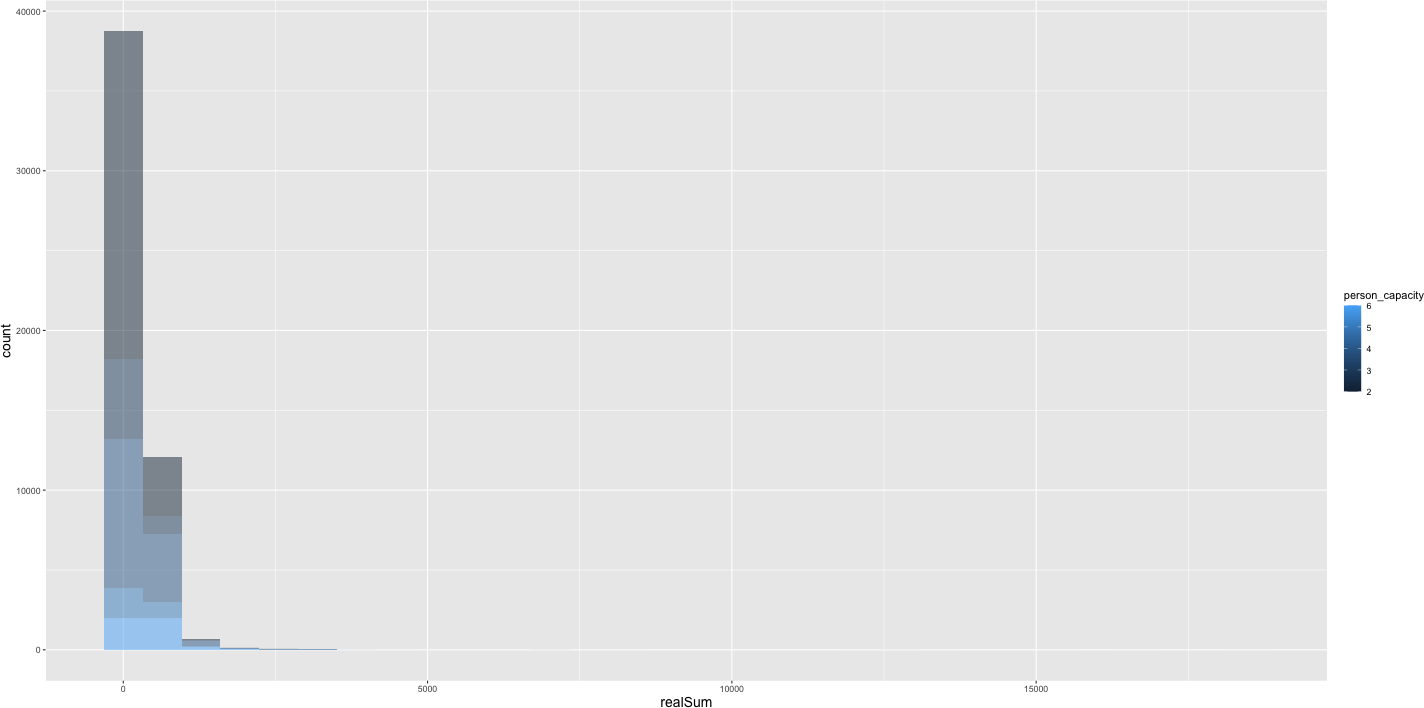
\includegraphics{Project_files/figure-latex/unnamed-chunk-19-1.png}

\begin{Shaded}
\begin{Highlighting}[]
\FunctionTok{ggplot}\NormalTok{(my\_data\_filtered, }\FunctionTok{aes}\NormalTok{(}\AttributeTok{x =}\NormalTok{ realSum, }\AttributeTok{fill =}\NormalTok{ person\_capacity,}
    \AttributeTok{group =}\NormalTok{ person\_capacity)) }\SpecialCharTok{+} \FunctionTok{geom\_histogram}\NormalTok{(}\AttributeTok{alpha =} \FloatTok{0.5}\NormalTok{, }\AttributeTok{nbins =} \DecValTok{20}\NormalTok{) }\SpecialCharTok{+}
    \FunctionTok{theme}\NormalTok{(}\AttributeTok{axis.title.x =} \FunctionTok{element\_text}\NormalTok{(}\AttributeTok{size =} \DecValTok{14}\NormalTok{), }\AttributeTok{axis.title.y =} \FunctionTok{element\_text}\NormalTok{(}\AttributeTok{size =} \DecValTok{14}\NormalTok{))}
\end{Highlighting}
\end{Shaded}

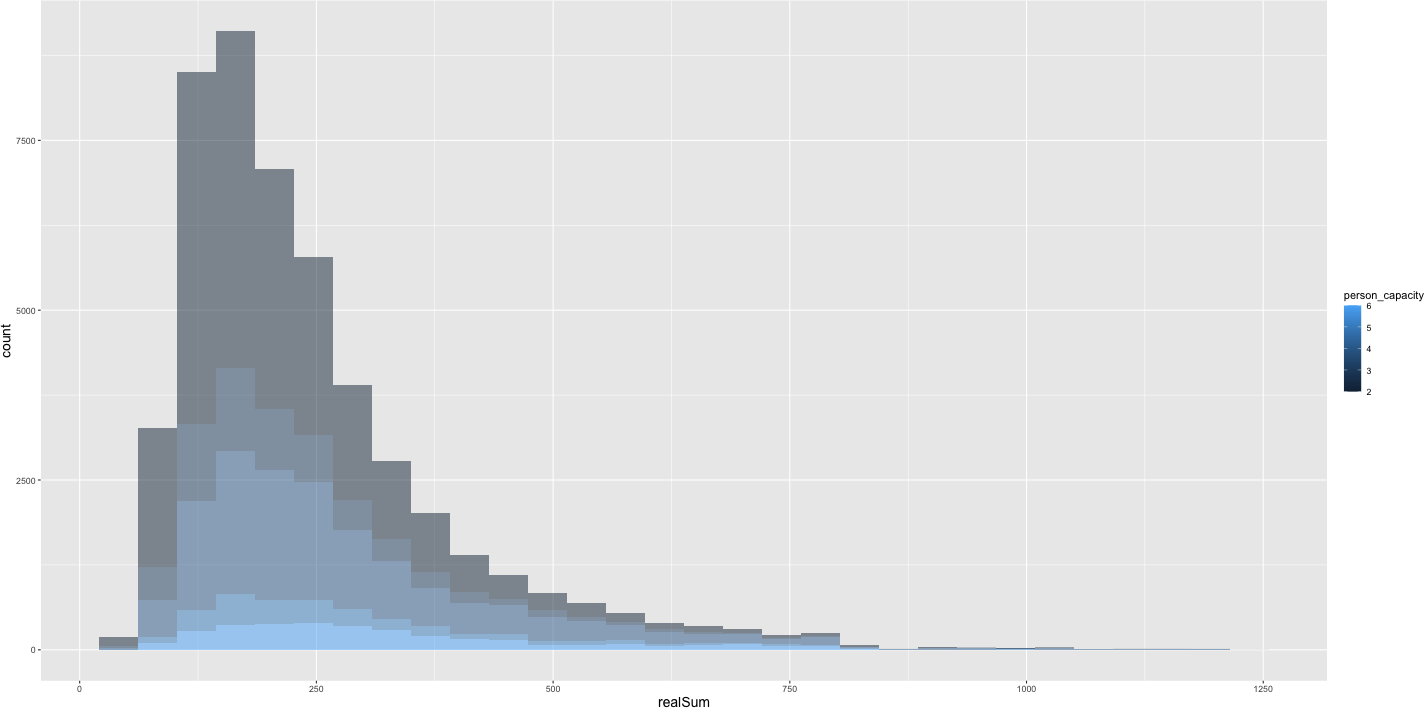
\includegraphics{Project_files/figure-latex/unnamed-chunk-19-2.png}

\begin{Shaded}
\begin{Highlighting}[]
\FunctionTok{ggplot}\NormalTok{(my\_data\_filtered, }\FunctionTok{aes}\NormalTok{(}\AttributeTok{x =}\NormalTok{ realSum, }\AttributeTok{fill =}\NormalTok{ person\_capacity,}
    \AttributeTok{group =}\NormalTok{ person\_capacity)) }\SpecialCharTok{+} \FunctionTok{geom\_histogram}\NormalTok{(}\AttributeTok{alpha =} \FloatTok{0.5}\NormalTok{, }\AttributeTok{nbins =} \DecValTok{20}\NormalTok{) }\SpecialCharTok{+}
    \FunctionTok{theme}\NormalTok{(}\AttributeTok{axis.title.x =} \FunctionTok{element\_text}\NormalTok{(}\AttributeTok{size =} \DecValTok{14}\NormalTok{), }\AttributeTok{axis.title.y =} \FunctionTok{element\_text}\NormalTok{(}\AttributeTok{size =} \DecValTok{14}\NormalTok{)) }\SpecialCharTok{+}
    \FunctionTok{facet\_wrap}\NormalTok{(}\SpecialCharTok{\textasciitilde{}}\NormalTok{city\_day)}
\end{Highlighting}
\end{Shaded}

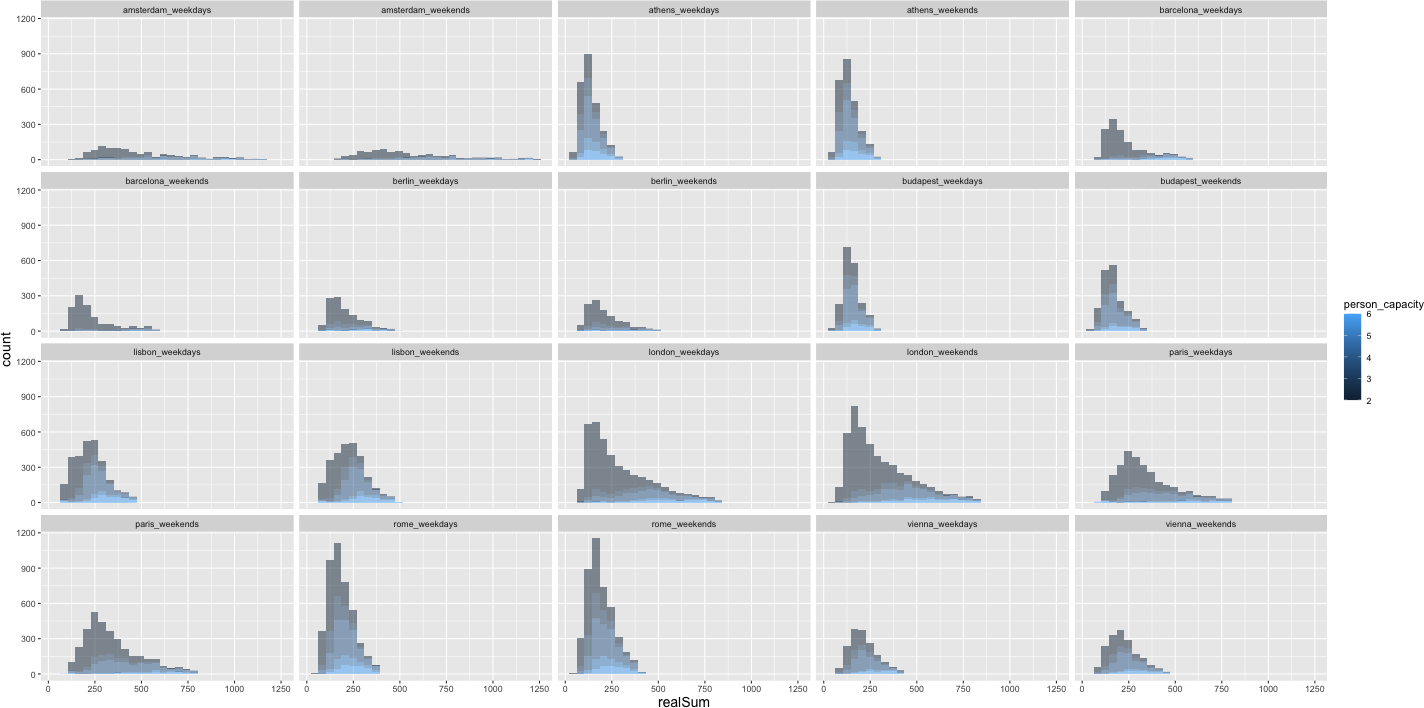
\includegraphics{Project_files/figure-latex/unnamed-chunk-19-3.png}

The overall price is distributed similarly across the spectrum
irrespective of person\_capacity. But for some cities like london,
london\_weekdays, lisbon the price is higher with person capacity. So,
person capacity along with city will be an important variable for
determining price.

\hypertarget{real-sum-vs-host_is_superhost}{%
\subsubsection{Real Sum Vs
host\_is\_superhost}\label{real-sum-vs-host_is_superhost}}

\begin{Shaded}
\begin{Highlighting}[]
\FunctionTok{ggplot}\NormalTok{(my\_data, }\FunctionTok{aes}\NormalTok{(}\AttributeTok{x =}\NormalTok{ realSum, }\AttributeTok{fill =}\NormalTok{ host\_is\_superhost, }\AttributeTok{group =}\NormalTok{ host\_is\_superhost)) }\SpecialCharTok{+}
    \FunctionTok{geom\_histogram}\NormalTok{(}\AttributeTok{alpha =} \FloatTok{0.5}\NormalTok{, }\AttributeTok{nbins =} \DecValTok{20}\NormalTok{) }\SpecialCharTok{+} \FunctionTok{theme}\NormalTok{(}\AttributeTok{axis.title.x =} \FunctionTok{element\_text}\NormalTok{(}\AttributeTok{size =} \DecValTok{14}\NormalTok{),}
    \AttributeTok{axis.title.y =} \FunctionTok{element\_text}\NormalTok{(}\AttributeTok{size =} \DecValTok{14}\NormalTok{))}
\end{Highlighting}
\end{Shaded}

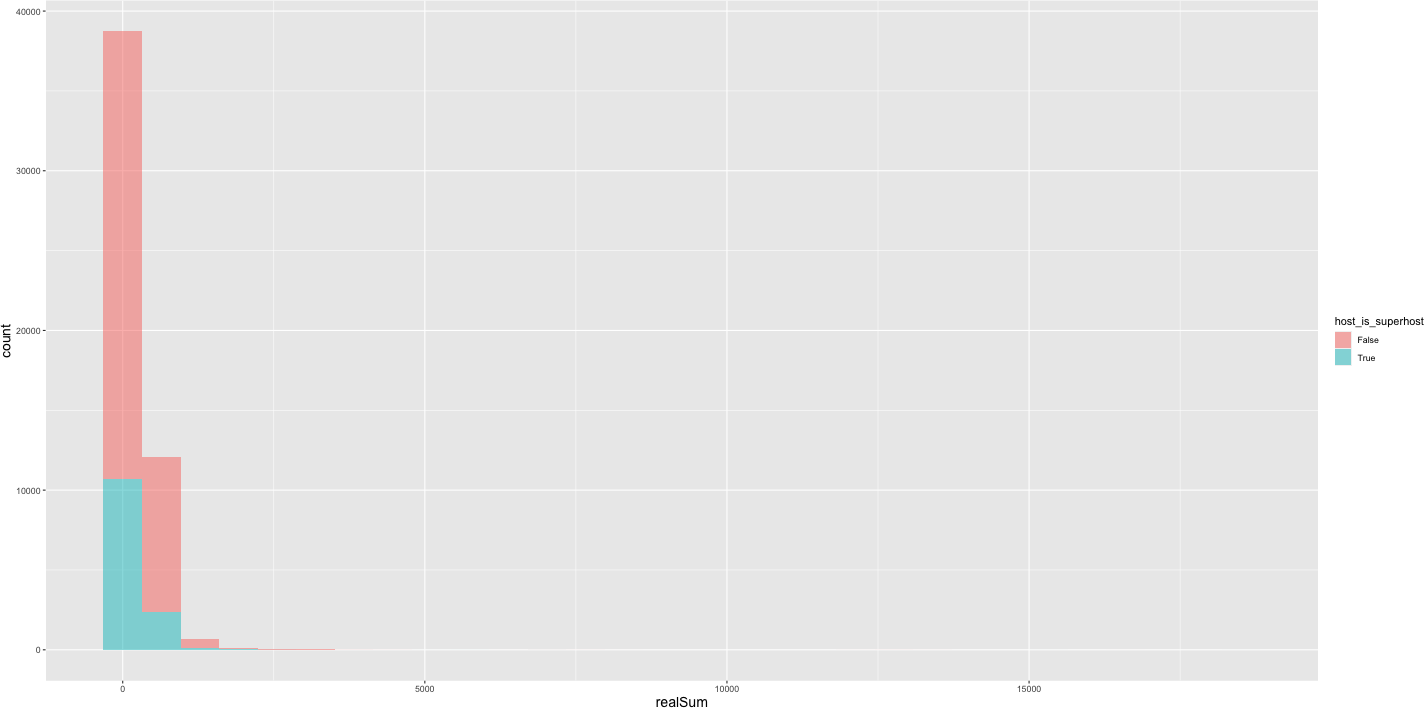
\includegraphics{Project_files/figure-latex/unnamed-chunk-20-1.png}

\begin{Shaded}
\begin{Highlighting}[]
\FunctionTok{ggplot}\NormalTok{(my\_data\_filtered, }\FunctionTok{aes}\NormalTok{(}\AttributeTok{x =}\NormalTok{ realSum, }\AttributeTok{fill =}\NormalTok{ host\_is\_superhost,}
    \AttributeTok{group =}\NormalTok{ host\_is\_superhost)) }\SpecialCharTok{+} \FunctionTok{geom\_histogram}\NormalTok{(}\AttributeTok{alpha =} \FloatTok{0.5}\NormalTok{,}
    \AttributeTok{nbins =} \DecValTok{20}\NormalTok{) }\SpecialCharTok{+} \FunctionTok{theme}\NormalTok{(}\AttributeTok{axis.title.x =} \FunctionTok{element\_text}\NormalTok{(}\AttributeTok{size =} \DecValTok{14}\NormalTok{),}
    \AttributeTok{axis.title.y =} \FunctionTok{element\_text}\NormalTok{(}\AttributeTok{size =} \DecValTok{14}\NormalTok{))}
\end{Highlighting}
\end{Shaded}

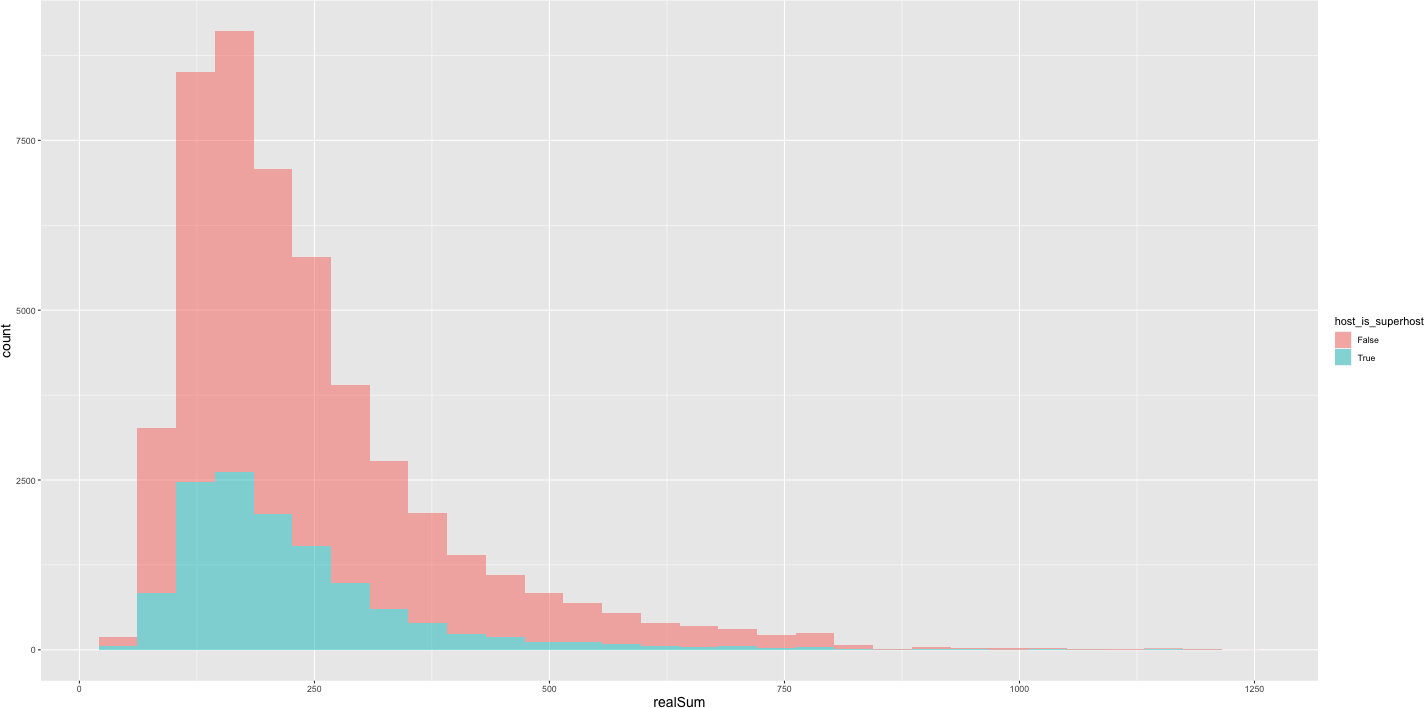
\includegraphics{Project_files/figure-latex/unnamed-chunk-20-2.png}

\begin{Shaded}
\begin{Highlighting}[]
\FunctionTok{ggplot}\NormalTok{(my\_data\_filtered, }\FunctionTok{aes}\NormalTok{(}\AttributeTok{x =}\NormalTok{ realSum, }\AttributeTok{fill =}\NormalTok{ host\_is\_superhost,}
    \AttributeTok{group =}\NormalTok{ host\_is\_superhost)) }\SpecialCharTok{+} \FunctionTok{geom\_histogram}\NormalTok{(}\AttributeTok{alpha =} \FloatTok{0.5}\NormalTok{,}
    \AttributeTok{nbins =} \DecValTok{20}\NormalTok{) }\SpecialCharTok{+} \FunctionTok{theme}\NormalTok{(}\AttributeTok{axis.title.x =} \FunctionTok{element\_text}\NormalTok{(}\AttributeTok{size =} \DecValTok{14}\NormalTok{),}
    \AttributeTok{axis.title.y =} \FunctionTok{element\_text}\NormalTok{(}\AttributeTok{size =} \DecValTok{14}\NormalTok{)) }\SpecialCharTok{+} \FunctionTok{facet\_wrap}\NormalTok{(}\SpecialCharTok{\textasciitilde{}}\NormalTok{city\_day)}
\end{Highlighting}
\end{Shaded}

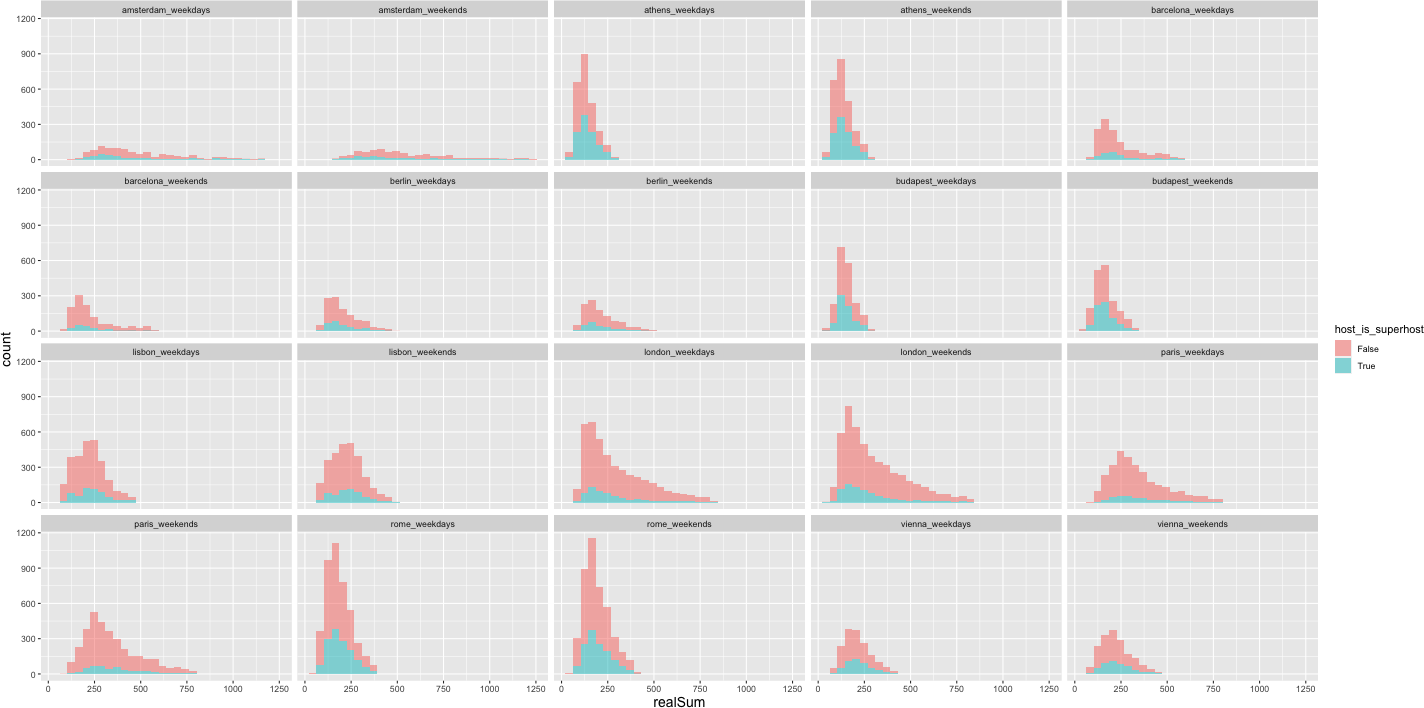
\includegraphics{Project_files/figure-latex/unnamed-chunk-20-3.png}

The prices are spread across all the spectrum irrespective of
super\_host or not.

\hypertarget{real-sum-vs-multi}{%
\subsubsection{Real Sum Vs multi}\label{real-sum-vs-multi}}

\begin{Shaded}
\begin{Highlighting}[]
\FunctionTok{ggplot}\NormalTok{(my\_data, }\FunctionTok{aes}\NormalTok{(}\AttributeTok{x =}\NormalTok{ realSum, }\AttributeTok{fill =}\NormalTok{ multi, }\AttributeTok{group =}\NormalTok{ multi)) }\SpecialCharTok{+}
    \FunctionTok{geom\_histogram}\NormalTok{(}\AttributeTok{alpha =} \FloatTok{0.5}\NormalTok{, }\AttributeTok{nbins =} \DecValTok{20}\NormalTok{) }\SpecialCharTok{+} \FunctionTok{theme}\NormalTok{(}\AttributeTok{axis.title.x =} \FunctionTok{element\_text}\NormalTok{(}\AttributeTok{size =} \DecValTok{14}\NormalTok{),}
    \AttributeTok{axis.title.y =} \FunctionTok{element\_text}\NormalTok{(}\AttributeTok{size =} \DecValTok{14}\NormalTok{))}
\end{Highlighting}
\end{Shaded}

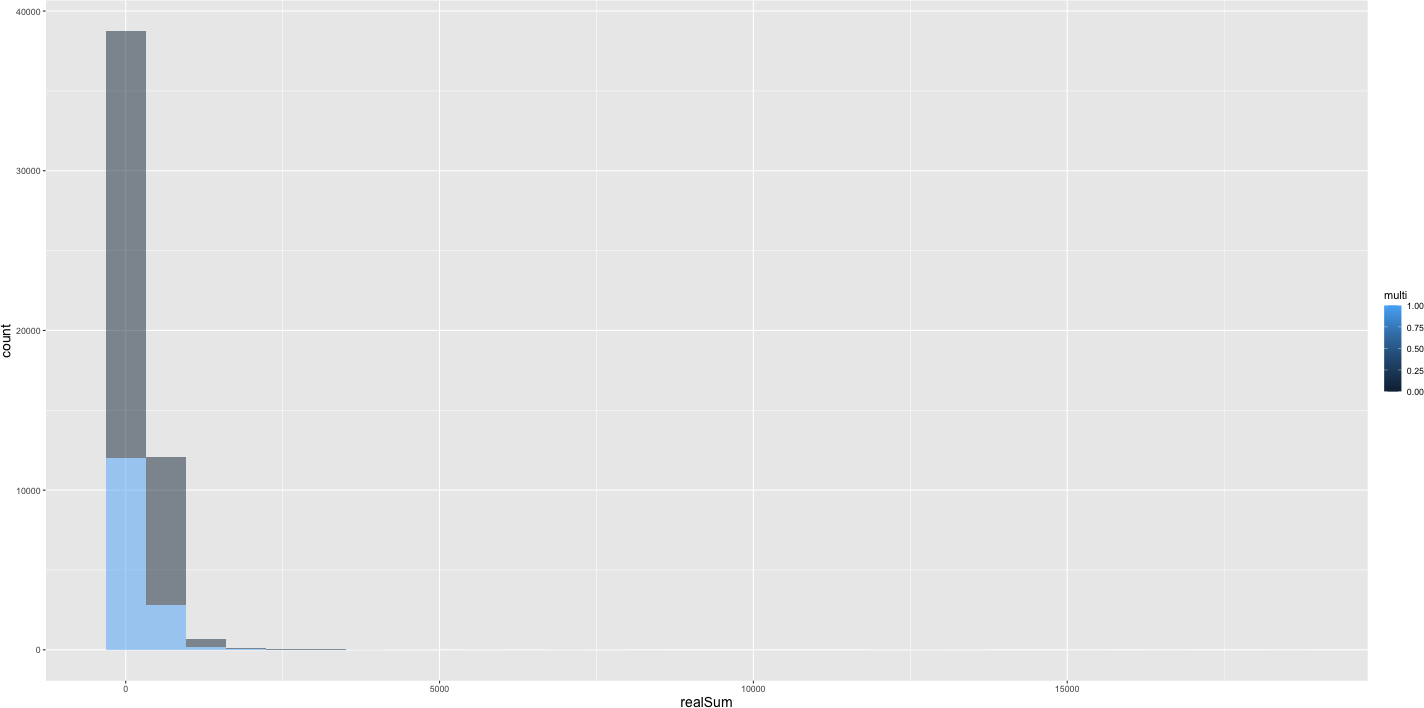
\includegraphics{Project_files/figure-latex/unnamed-chunk-21-1.png}

\begin{Shaded}
\begin{Highlighting}[]
\FunctionTok{ggplot}\NormalTok{(my\_data\_filtered, }\FunctionTok{aes}\NormalTok{(}\AttributeTok{x =}\NormalTok{ realSum, }\AttributeTok{fill =}\NormalTok{ multi, }\AttributeTok{group =}\NormalTok{ multi)) }\SpecialCharTok{+}
    \FunctionTok{geom\_histogram}\NormalTok{(}\AttributeTok{alpha =} \FloatTok{0.5}\NormalTok{, }\AttributeTok{nbins =} \DecValTok{20}\NormalTok{) }\SpecialCharTok{+} \FunctionTok{theme}\NormalTok{(}\AttributeTok{axis.title.x =} \FunctionTok{element\_text}\NormalTok{(}\AttributeTok{size =} \DecValTok{14}\NormalTok{),}
    \AttributeTok{axis.title.y =} \FunctionTok{element\_text}\NormalTok{(}\AttributeTok{size =} \DecValTok{14}\NormalTok{))}
\end{Highlighting}
\end{Shaded}

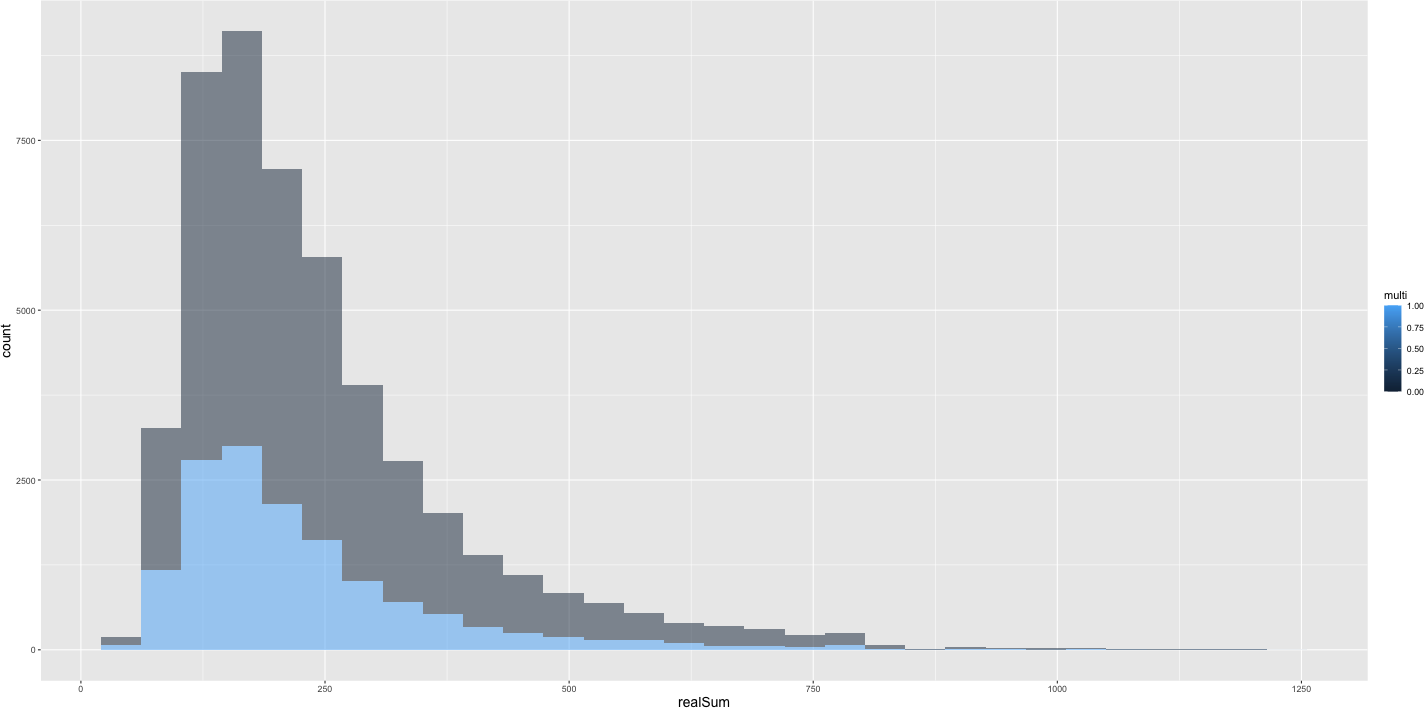
\includegraphics{Project_files/figure-latex/unnamed-chunk-21-2.png}

\begin{Shaded}
\begin{Highlighting}[]
\FunctionTok{ggplot}\NormalTok{(my\_data\_filtered, }\FunctionTok{aes}\NormalTok{(}\AttributeTok{x =}\NormalTok{ realSum, }\AttributeTok{fill =}\NormalTok{ multi, }\AttributeTok{group =}\NormalTok{ multi)) }\SpecialCharTok{+}
    \FunctionTok{geom\_histogram}\NormalTok{(}\AttributeTok{alpha =} \FloatTok{0.5}\NormalTok{, }\AttributeTok{nbins =} \DecValTok{20}\NormalTok{) }\SpecialCharTok{+} \FunctionTok{theme}\NormalTok{(}\AttributeTok{axis.title.x =} \FunctionTok{element\_text}\NormalTok{(}\AttributeTok{size =} \DecValTok{14}\NormalTok{),}
    \AttributeTok{axis.title.y =} \FunctionTok{element\_text}\NormalTok{(}\AttributeTok{size =} \DecValTok{14}\NormalTok{)) }\SpecialCharTok{+} \FunctionTok{facet\_wrap}\NormalTok{(}\SpecialCharTok{\textasciitilde{}}\NormalTok{city\_day)}
\end{Highlighting}
\end{Shaded}

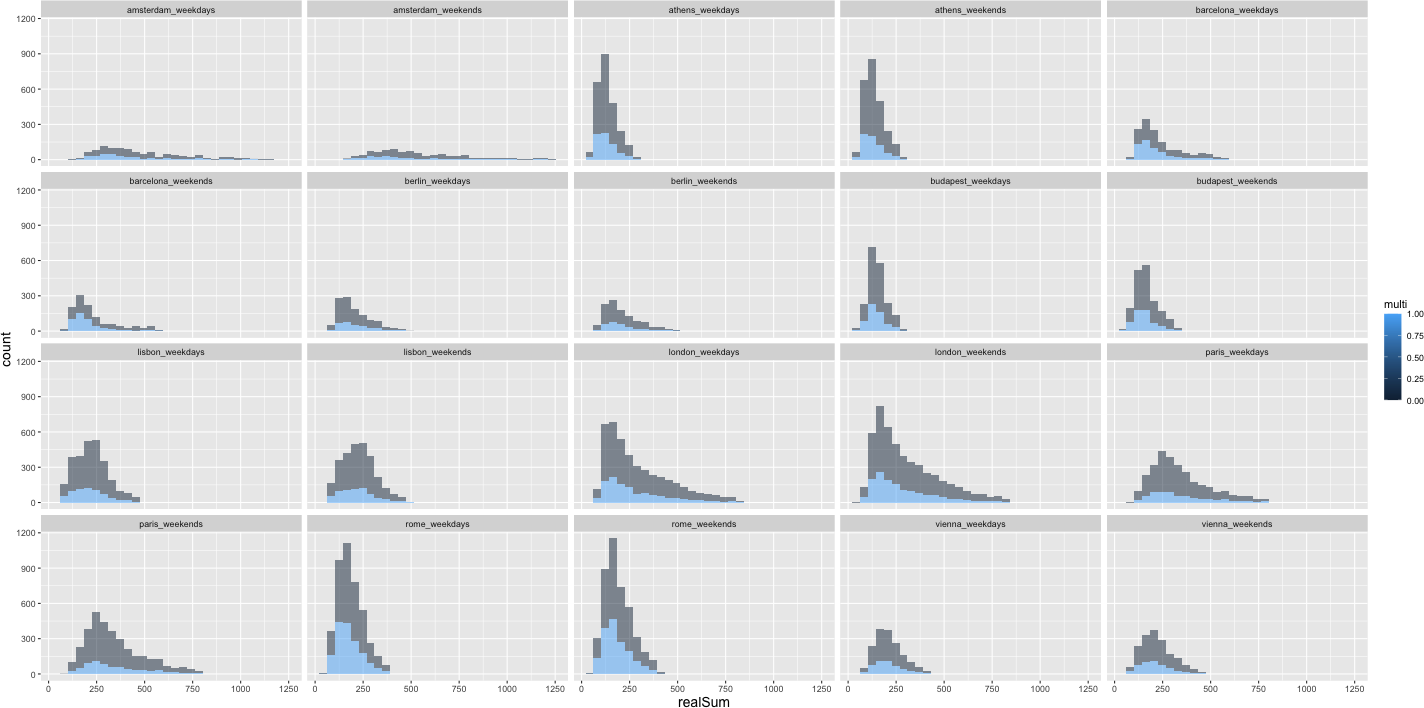
\includegraphics{Project_files/figure-latex/unnamed-chunk-21-3.png}

The prices are similar irrespective of multi or not.

\hypertarget{real-sum-vs-biz}{%
\subsubsection{Real Sum Vs biz}\label{real-sum-vs-biz}}

\begin{Shaded}
\begin{Highlighting}[]
\FunctionTok{ggplot}\NormalTok{(my\_data, }\FunctionTok{aes}\NormalTok{(}\AttributeTok{x =}\NormalTok{ realSum, }\AttributeTok{fill =}\NormalTok{ biz, }\AttributeTok{group =}\NormalTok{ biz)) }\SpecialCharTok{+}
    \FunctionTok{geom\_histogram}\NormalTok{(}\AttributeTok{alpha =} \FloatTok{0.5}\NormalTok{, }\AttributeTok{nbins =} \DecValTok{20}\NormalTok{) }\SpecialCharTok{+} \FunctionTok{theme}\NormalTok{(}\AttributeTok{axis.title.x =} \FunctionTok{element\_text}\NormalTok{(}\AttributeTok{size =} \DecValTok{14}\NormalTok{),}
    \AttributeTok{axis.title.y =} \FunctionTok{element\_text}\NormalTok{(}\AttributeTok{size =} \DecValTok{14}\NormalTok{))}
\end{Highlighting}
\end{Shaded}

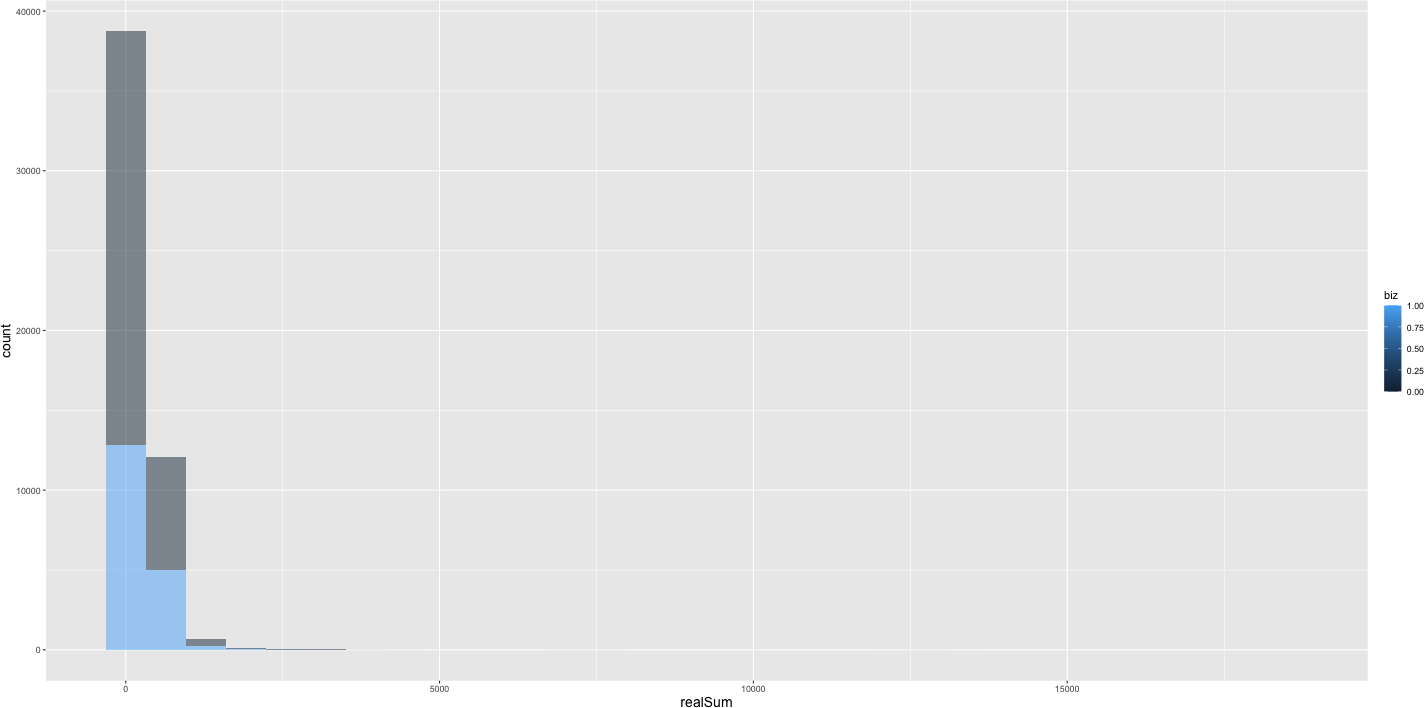
\includegraphics{Project_files/figure-latex/unnamed-chunk-22-1.png}

\begin{Shaded}
\begin{Highlighting}[]
\FunctionTok{ggplot}\NormalTok{(my\_data\_filtered, }\FunctionTok{aes}\NormalTok{(}\AttributeTok{x =}\NormalTok{ realSum, }\AttributeTok{fill =}\NormalTok{ biz, }\AttributeTok{group =}\NormalTok{ biz)) }\SpecialCharTok{+}
    \FunctionTok{geom\_histogram}\NormalTok{(}\AttributeTok{alpha =} \FloatTok{0.5}\NormalTok{, }\AttributeTok{nbins =} \DecValTok{20}\NormalTok{) }\SpecialCharTok{+} \FunctionTok{theme}\NormalTok{(}\AttributeTok{axis.title.x =} \FunctionTok{element\_text}\NormalTok{(}\AttributeTok{size =} \DecValTok{14}\NormalTok{),}
    \AttributeTok{axis.title.y =} \FunctionTok{element\_text}\NormalTok{(}\AttributeTok{size =} \DecValTok{14}\NormalTok{))}
\end{Highlighting}
\end{Shaded}

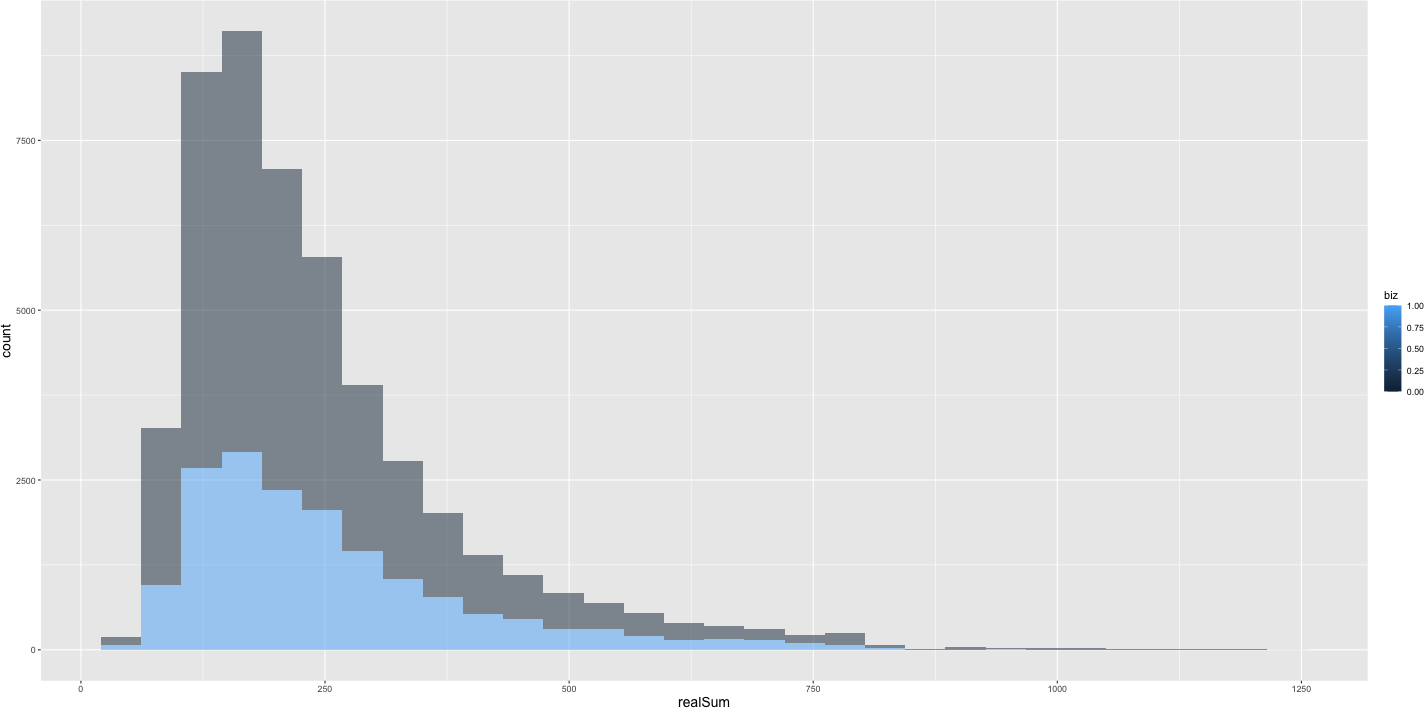
\includegraphics{Project_files/figure-latex/unnamed-chunk-22-2.png}

\begin{Shaded}
\begin{Highlighting}[]
\FunctionTok{ggplot}\NormalTok{(my\_data\_filtered, }\FunctionTok{aes}\NormalTok{(}\AttributeTok{x =}\NormalTok{ realSum, }\AttributeTok{fill =}\NormalTok{ biz, }\AttributeTok{group =}\NormalTok{ biz)) }\SpecialCharTok{+}
    \FunctionTok{geom\_histogram}\NormalTok{(}\AttributeTok{alpha =} \FloatTok{0.5}\NormalTok{, }\AttributeTok{nbins =} \DecValTok{20}\NormalTok{) }\SpecialCharTok{+} \FunctionTok{theme}\NormalTok{(}\AttributeTok{axis.title.x =} \FunctionTok{element\_text}\NormalTok{(}\AttributeTok{size =} \DecValTok{14}\NormalTok{),}
    \AttributeTok{axis.title.y =} \FunctionTok{element\_text}\NormalTok{(}\AttributeTok{size =} \DecValTok{14}\NormalTok{)) }\SpecialCharTok{+} \FunctionTok{facet\_wrap}\NormalTok{(}\SpecialCharTok{\textasciitilde{}}\NormalTok{city\_day)}
\end{Highlighting}
\end{Shaded}

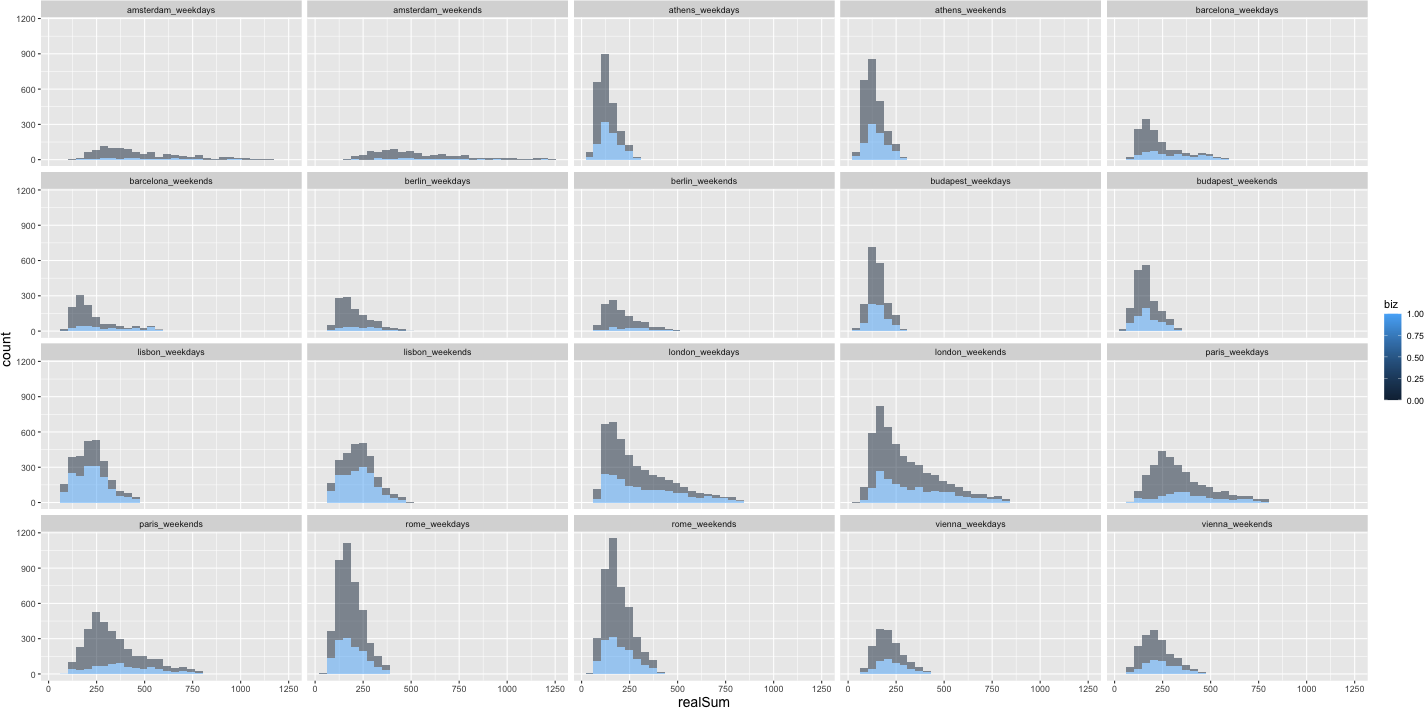
\includegraphics{Project_files/figure-latex/unnamed-chunk-22-3.png}

The prices are similar irrespective of biz or not.

\hypertarget{real-sum-vs-cleanliness}{%
\subsubsection{Real Sum vs Cleanliness}\label{real-sum-vs-cleanliness}}

\begin{Shaded}
\begin{Highlighting}[]
\FunctionTok{ggplot}\NormalTok{(my\_data, }\FunctionTok{aes}\NormalTok{(}\AttributeTok{x =}\NormalTok{ realSum, }\AttributeTok{fill =}\NormalTok{ cleanliness\_rating, }\AttributeTok{group =}\NormalTok{ cleanliness\_rating)) }\SpecialCharTok{+}
    \FunctionTok{geom\_histogram}\NormalTok{(}\AttributeTok{alpha =} \FloatTok{0.5}\NormalTok{, }\AttributeTok{nbins =} \DecValTok{20}\NormalTok{) }\SpecialCharTok{+} \FunctionTok{theme}\NormalTok{(}\AttributeTok{axis.title.x =} \FunctionTok{element\_text}\NormalTok{(}\AttributeTok{size =} \DecValTok{14}\NormalTok{),}
    \AttributeTok{axis.title.y =} \FunctionTok{element\_text}\NormalTok{(}\AttributeTok{size =} \DecValTok{14}\NormalTok{))}
\end{Highlighting}
\end{Shaded}

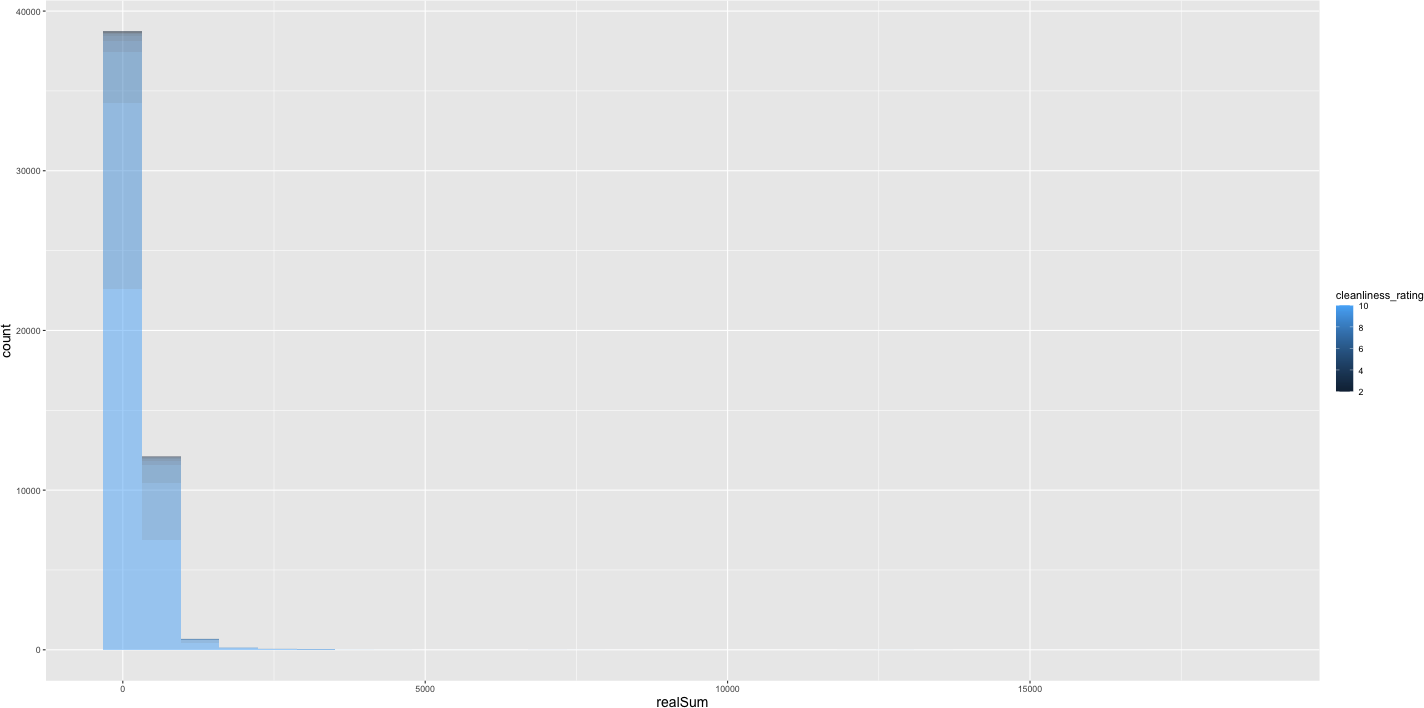
\includegraphics{Project_files/figure-latex/unnamed-chunk-23-1.png}

\begin{Shaded}
\begin{Highlighting}[]
\FunctionTok{ggplot}\NormalTok{(my\_data\_filtered, }\FunctionTok{aes}\NormalTok{(}\AttributeTok{x =}\NormalTok{ realSum, }\AttributeTok{fill =}\NormalTok{ cleanliness\_rating,}
    \AttributeTok{group =}\NormalTok{ cleanliness\_rating)) }\SpecialCharTok{+} \FunctionTok{geom\_histogram}\NormalTok{(}\AttributeTok{alpha =} \FloatTok{0.5}\NormalTok{,}
    \AttributeTok{nbins =} \DecValTok{20}\NormalTok{) }\SpecialCharTok{+} \FunctionTok{theme}\NormalTok{(}\AttributeTok{axis.title.x =} \FunctionTok{element\_text}\NormalTok{(}\AttributeTok{size =} \DecValTok{14}\NormalTok{),}
    \AttributeTok{axis.title.y =} \FunctionTok{element\_text}\NormalTok{(}\AttributeTok{size =} \DecValTok{14}\NormalTok{))}
\end{Highlighting}
\end{Shaded}

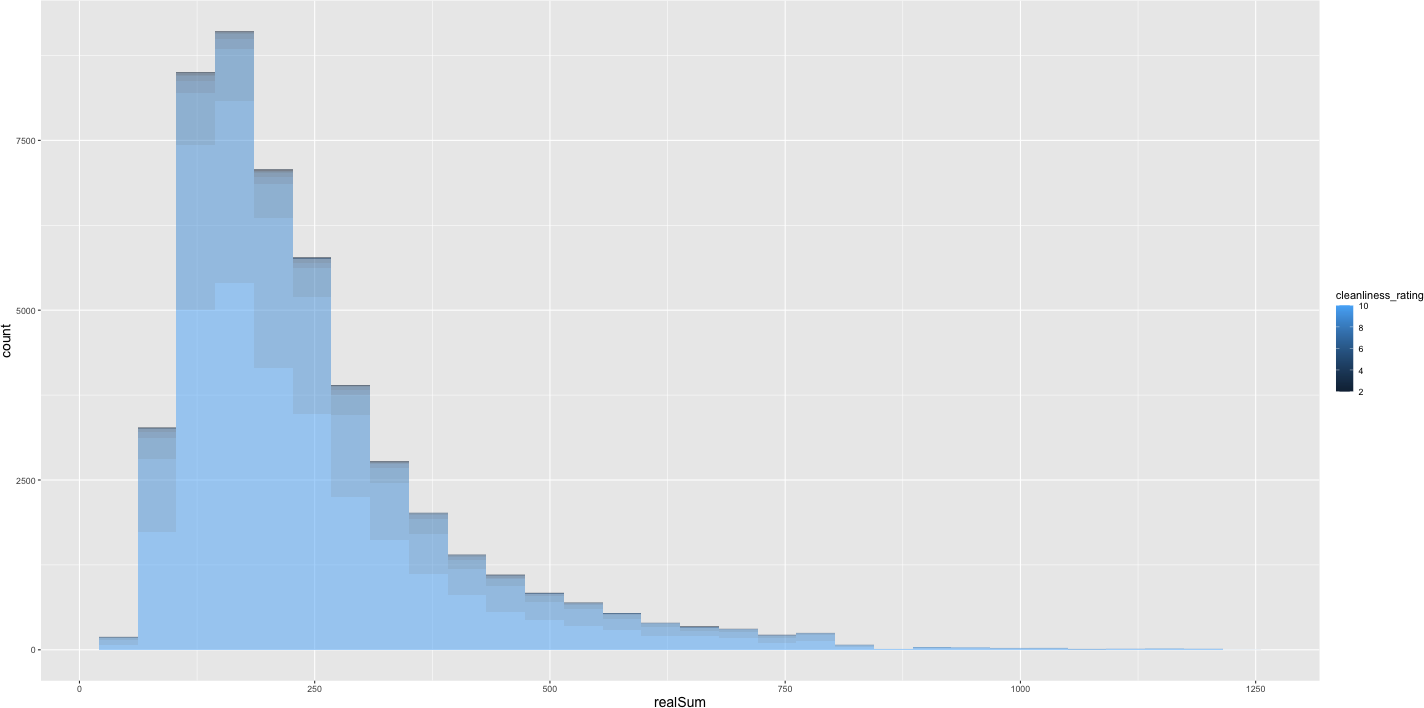
\includegraphics{Project_files/figure-latex/unnamed-chunk-23-2.png}

\begin{Shaded}
\begin{Highlighting}[]
\FunctionTok{ggplot}\NormalTok{(my\_data\_filtered, }\FunctionTok{aes}\NormalTok{(}\AttributeTok{x =}\NormalTok{ realSum, }\AttributeTok{fill =}\NormalTok{ cleanliness\_rating,}
    \AttributeTok{group =}\NormalTok{ cleanliness\_rating)) }\SpecialCharTok{+} \FunctionTok{geom\_histogram}\NormalTok{(}\AttributeTok{alpha =} \FloatTok{0.5}\NormalTok{,}
    \AttributeTok{nbins =} \DecValTok{20}\NormalTok{) }\SpecialCharTok{+} \FunctionTok{theme}\NormalTok{(}\AttributeTok{axis.title.x =} \FunctionTok{element\_text}\NormalTok{(}\AttributeTok{size =} \DecValTok{14}\NormalTok{),}
    \AttributeTok{axis.title.y =} \FunctionTok{element\_text}\NormalTok{(}\AttributeTok{size =} \DecValTok{14}\NormalTok{)) }\SpecialCharTok{+} \FunctionTok{facet\_wrap}\NormalTok{(}\SpecialCharTok{\textasciitilde{}}\NormalTok{city\_day)}
\end{Highlighting}
\end{Shaded}

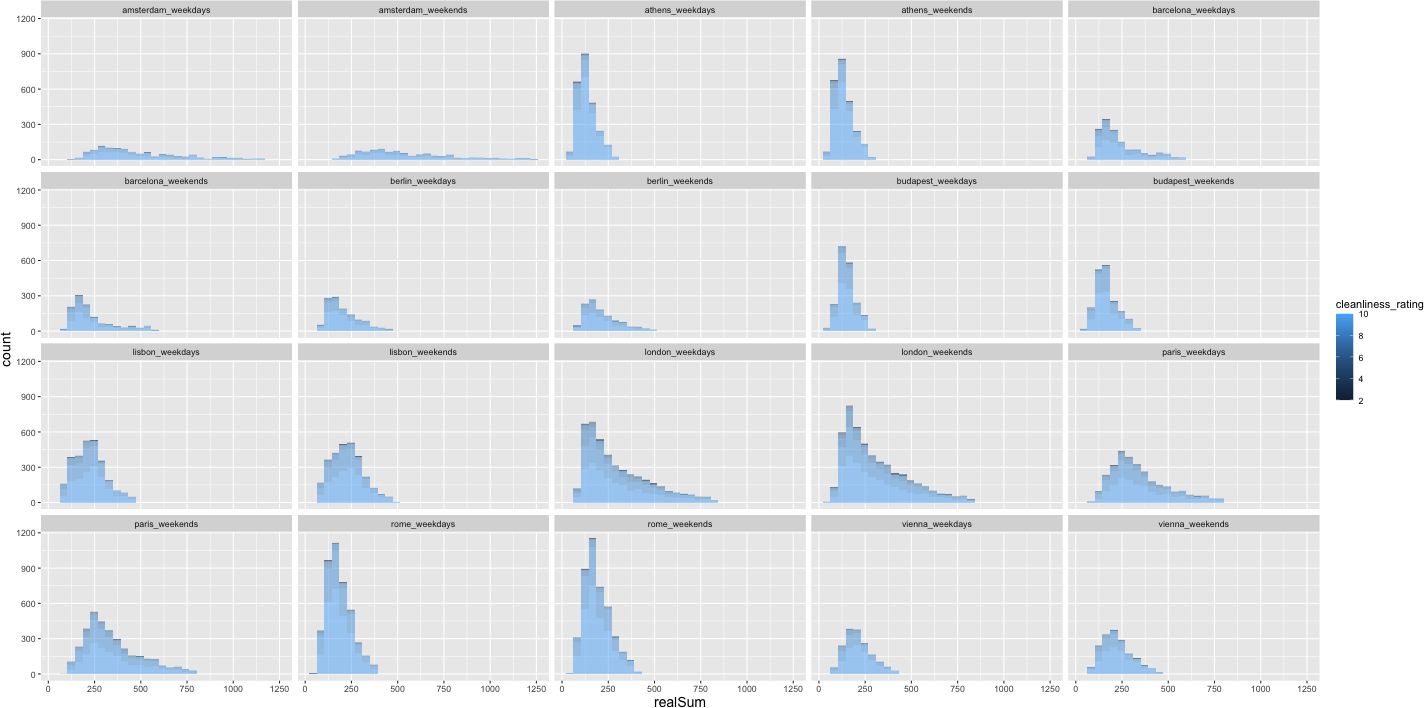
\includegraphics{Project_files/figure-latex/unnamed-chunk-23-3.png}

The cleanliness rating doesn't really have an effect on price

\hypertarget{scatterplot-of-price-vs-guest-satisfaction-filtered-by-city}{%
\subsubsection{Scatterplot of Price vs Guest Satisfaction filtered by
city}\label{scatterplot-of-price-vs-guest-satisfaction-filtered-by-city}}

\begin{Shaded}
\begin{Highlighting}[]
\FunctionTok{ggplot}\NormalTok{(my\_data\_filtered, }\FunctionTok{aes}\NormalTok{(}\AttributeTok{x =}\NormalTok{ realSum, }\AttributeTok{y =}\NormalTok{ guest\_satisfaction\_overall,}
    \AttributeTok{color =}\NormalTok{ city\_day)) }\SpecialCharTok{+} \FunctionTok{geom\_point}\NormalTok{() }\SpecialCharTok{+} \FunctionTok{xlab}\NormalTok{(}\StringTok{"Price"}\NormalTok{) }\SpecialCharTok{+} \FunctionTok{ylab}\NormalTok{(}\StringTok{"Guest Satisfaction Overall"}\NormalTok{) }\SpecialCharTok{+}
    \FunctionTok{scale\_color\_discrete}\NormalTok{(}\AttributeTok{name =} \StringTok{"City{-}Day"}\NormalTok{)}
\end{Highlighting}
\end{Shaded}

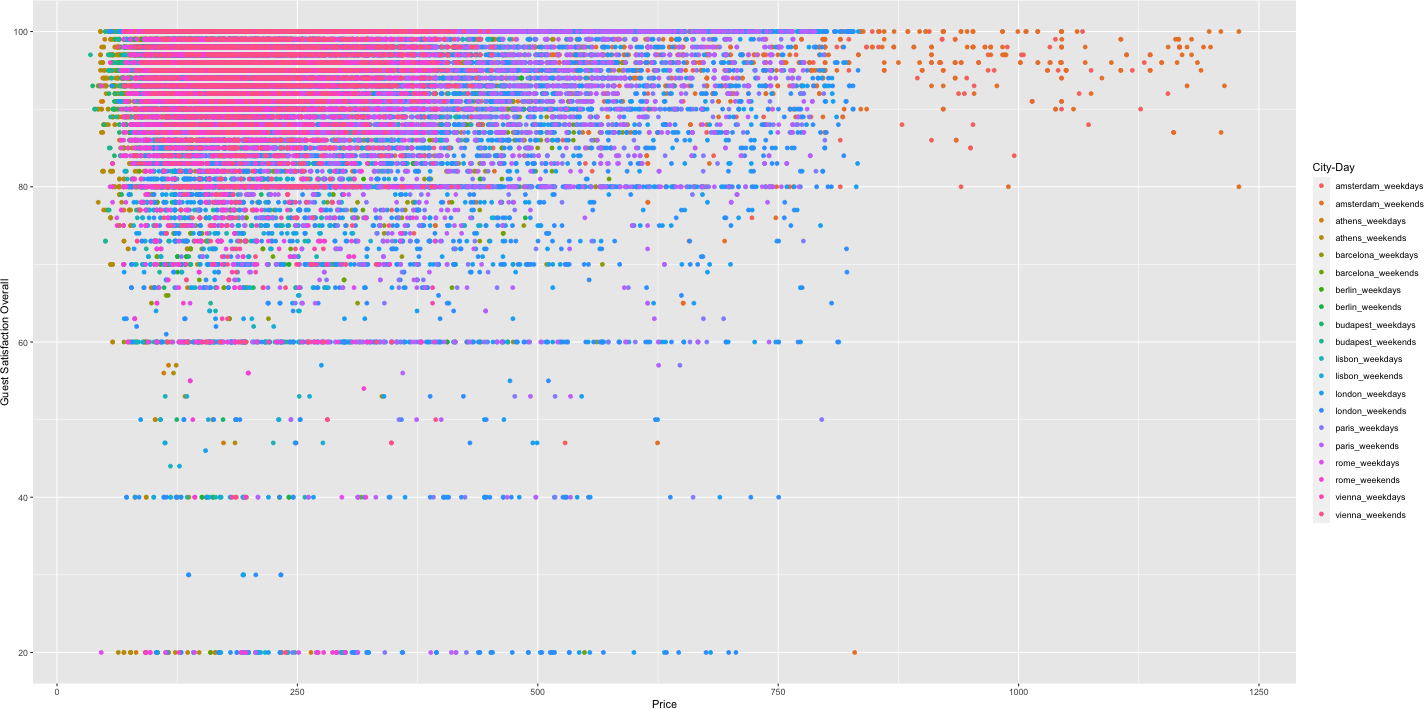
\includegraphics{Project_files/figure-latex/unnamed-chunk-24-1.png}

\begin{Shaded}
\begin{Highlighting}[]
\FunctionTok{ggplot}\NormalTok{(my\_data\_filtered, }\FunctionTok{aes}\NormalTok{(}\AttributeTok{x =}\NormalTok{ realSum, }\AttributeTok{y =}\NormalTok{ guest\_satisfaction\_overall,}
    \AttributeTok{color =}\NormalTok{ city\_day)) }\SpecialCharTok{+} \FunctionTok{geom\_point}\NormalTok{() }\SpecialCharTok{+} \FunctionTok{xlab}\NormalTok{(}\StringTok{"Price"}\NormalTok{) }\SpecialCharTok{+} \FunctionTok{ylab}\NormalTok{(}\StringTok{"Guest Satisfaction Overall"}\NormalTok{) }\SpecialCharTok{+}
    \FunctionTok{scale\_color\_discrete}\NormalTok{(}\AttributeTok{name =} \StringTok{"City{-}Day"}\NormalTok{) }\SpecialCharTok{+} \FunctionTok{facet\_wrap}\NormalTok{(}\SpecialCharTok{\textasciitilde{}}\NormalTok{city\_day)}
\end{Highlighting}
\end{Shaded}

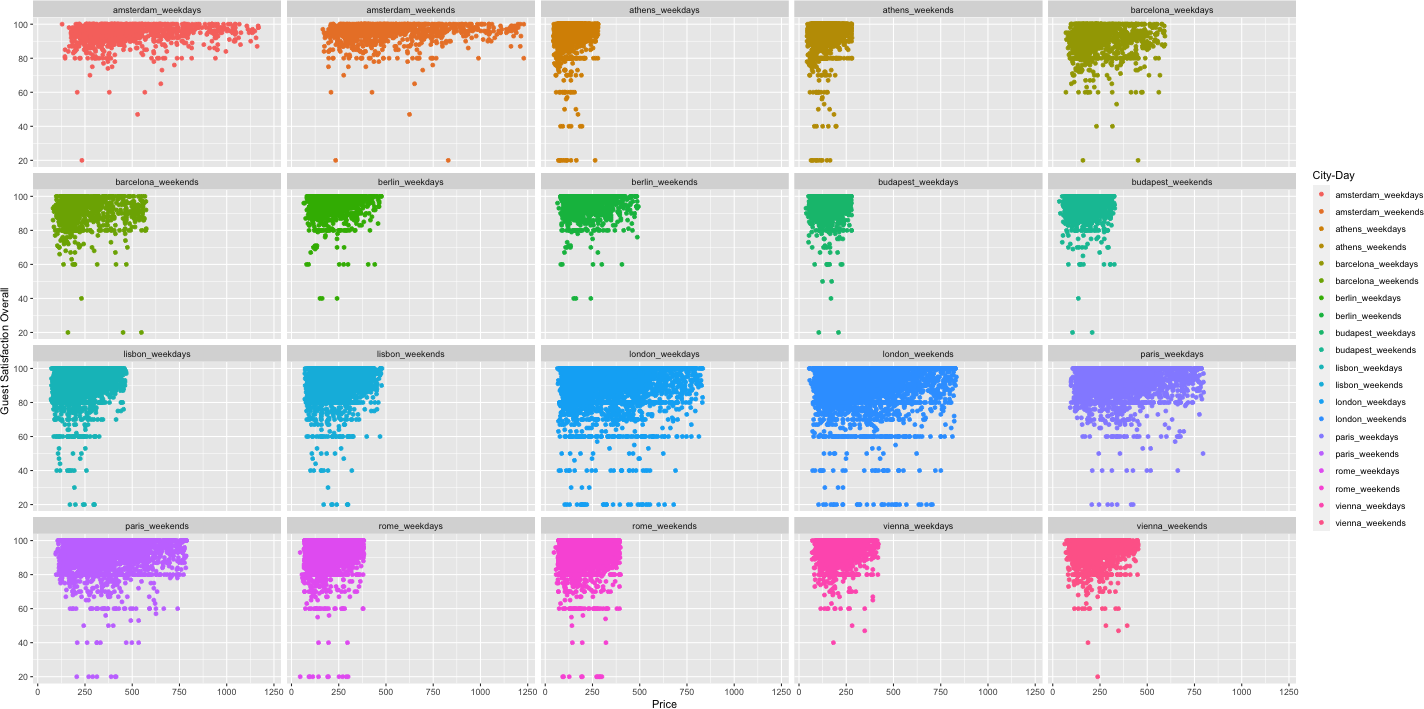
\includegraphics{Project_files/figure-latex/unnamed-chunk-24-2.png}

The plot depicts that there is no correlation of price with guest
satisfaction, good satisfaction rate is found across all the prices. In
some cities like lonon, we can see a group of reviews with low guest
satisfaction.

\hypertarget{real-sum-vs-bedroom-count}{%
\subsubsection{Real Sum Vs Bedroom
Count}\label{real-sum-vs-bedroom-count}}

\begin{Shaded}
\begin{Highlighting}[]
\FunctionTok{ggplot}\NormalTok{(my\_data, }\FunctionTok{aes}\NormalTok{(}\AttributeTok{x =}\NormalTok{ realSum, }\AttributeTok{fill =}\NormalTok{ bedrooms, }\AttributeTok{group =}\NormalTok{ bedrooms)) }\SpecialCharTok{+}
    \FunctionTok{geom\_histogram}\NormalTok{(}\AttributeTok{alpha =} \FloatTok{0.6}\NormalTok{) }\SpecialCharTok{+} \FunctionTok{theme}\NormalTok{(}\AttributeTok{axis.title.x =} \FunctionTok{element\_text}\NormalTok{(}\AttributeTok{size =} \DecValTok{14}\NormalTok{),}
    \AttributeTok{axis.title.y =} \FunctionTok{element\_text}\NormalTok{(}\AttributeTok{size =} \DecValTok{14}\NormalTok{))}
\end{Highlighting}
\end{Shaded}

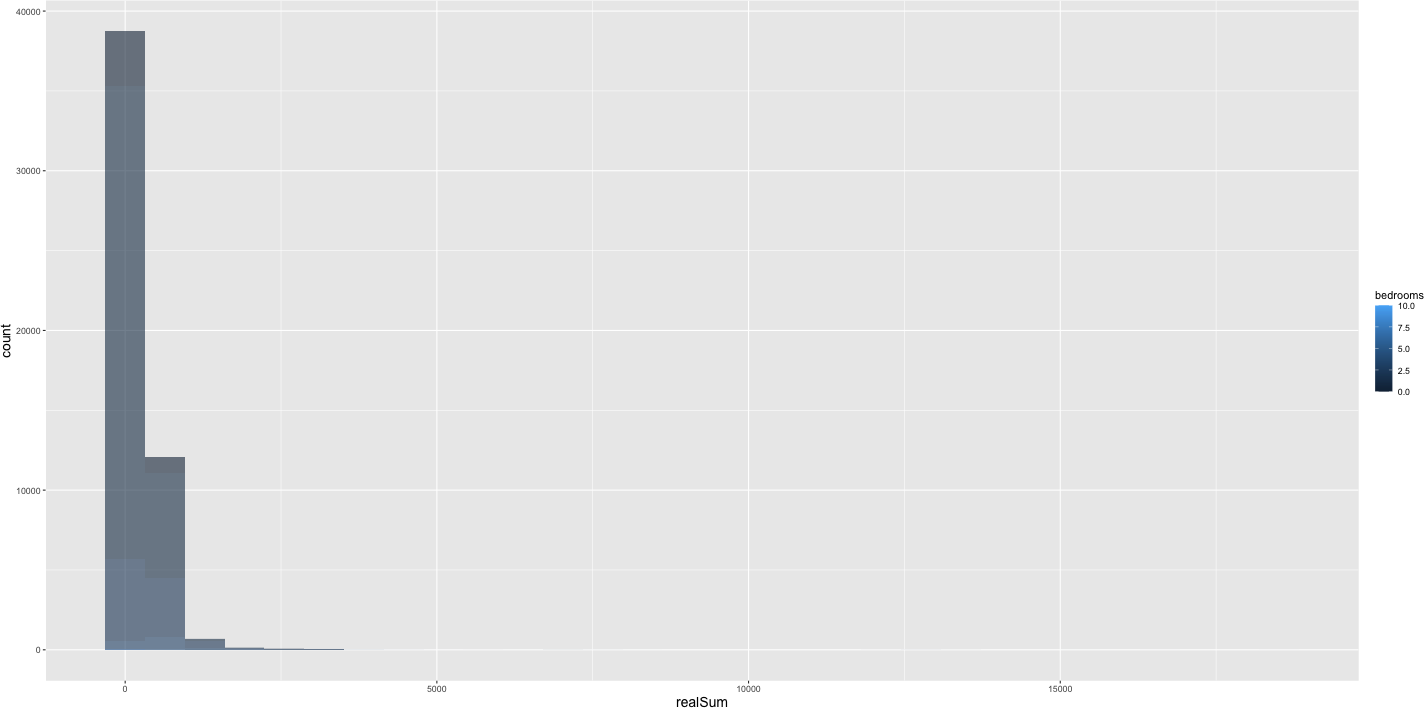
\includegraphics{Project_files/figure-latex/unnamed-chunk-25-1.png}

\begin{Shaded}
\begin{Highlighting}[]
\FunctionTok{ggplot}\NormalTok{(my\_data\_filtered, }\FunctionTok{aes}\NormalTok{(}\AttributeTok{x =}\NormalTok{ realSum, }\AttributeTok{fill =}\NormalTok{ bedrooms, }\AttributeTok{group =}\NormalTok{ bedrooms)) }\SpecialCharTok{+}
    \FunctionTok{geom\_histogram}\NormalTok{(}\AttributeTok{alpha =} \FloatTok{0.6}\NormalTok{) }\SpecialCharTok{+} \FunctionTok{theme}\NormalTok{(}\AttributeTok{axis.title.x =} \FunctionTok{element\_text}\NormalTok{(}\AttributeTok{size =} \DecValTok{14}\NormalTok{),}
    \AttributeTok{axis.title.y =} \FunctionTok{element\_text}\NormalTok{(}\AttributeTok{size =} \DecValTok{14}\NormalTok{))}
\end{Highlighting}
\end{Shaded}

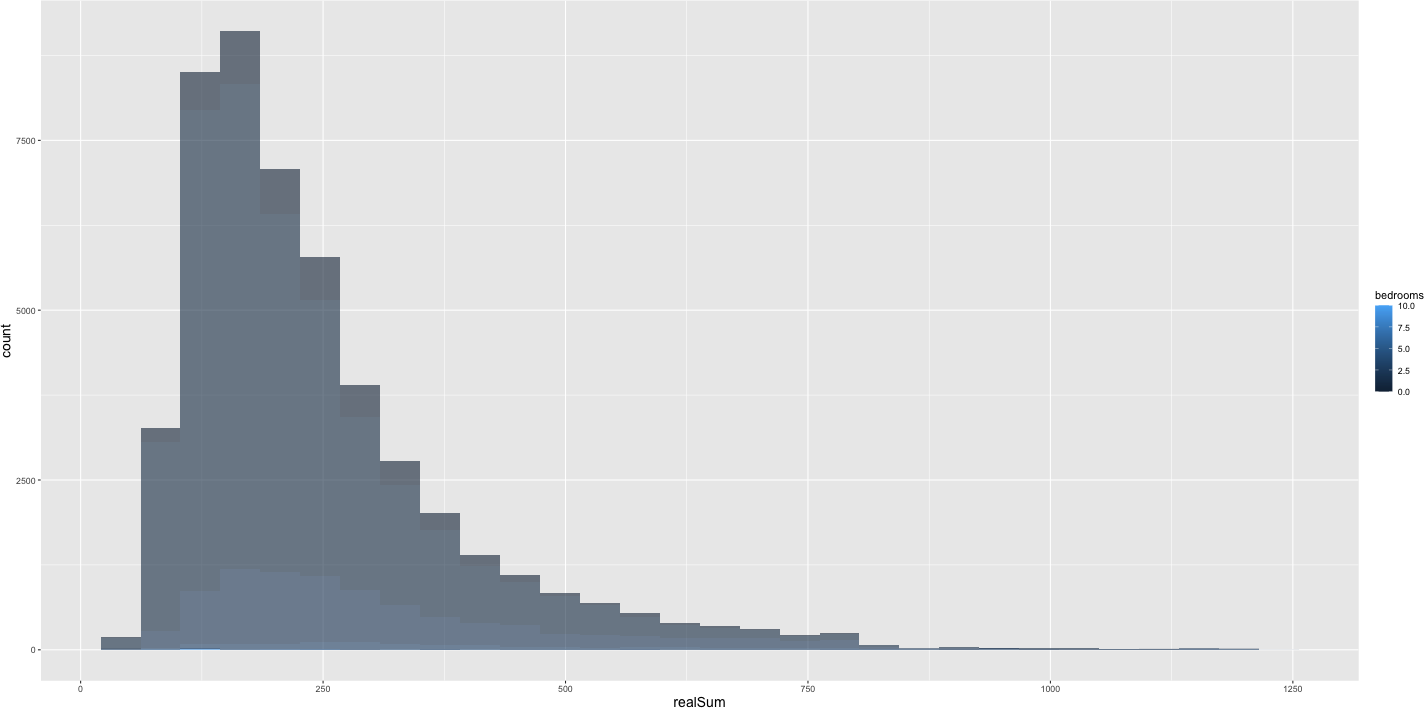
\includegraphics{Project_files/figure-latex/unnamed-chunk-25-2.png}

\begin{Shaded}
\begin{Highlighting}[]
\FunctionTok{ggplot}\NormalTok{(my\_data\_filtered, }\FunctionTok{aes}\NormalTok{(}\AttributeTok{x =}\NormalTok{ realSum, }\AttributeTok{fill =}\NormalTok{ bedrooms, }\AttributeTok{group =}\NormalTok{ bedrooms)) }\SpecialCharTok{+}
    \FunctionTok{geom\_histogram}\NormalTok{(}\AttributeTok{alpha =} \FloatTok{0.6}\NormalTok{) }\SpecialCharTok{+} \FunctionTok{theme}\NormalTok{(}\AttributeTok{axis.title.x =} \FunctionTok{element\_text}\NormalTok{(}\AttributeTok{size =} \DecValTok{14}\NormalTok{),}
    \AttributeTok{axis.title.y =} \FunctionTok{element\_text}\NormalTok{(}\AttributeTok{size =} \DecValTok{14}\NormalTok{)) }\SpecialCharTok{+} \FunctionTok{facet\_wrap}\NormalTok{(}\SpecialCharTok{\textasciitilde{}}\NormalTok{city\_day)}
\end{Highlighting}
\end{Shaded}

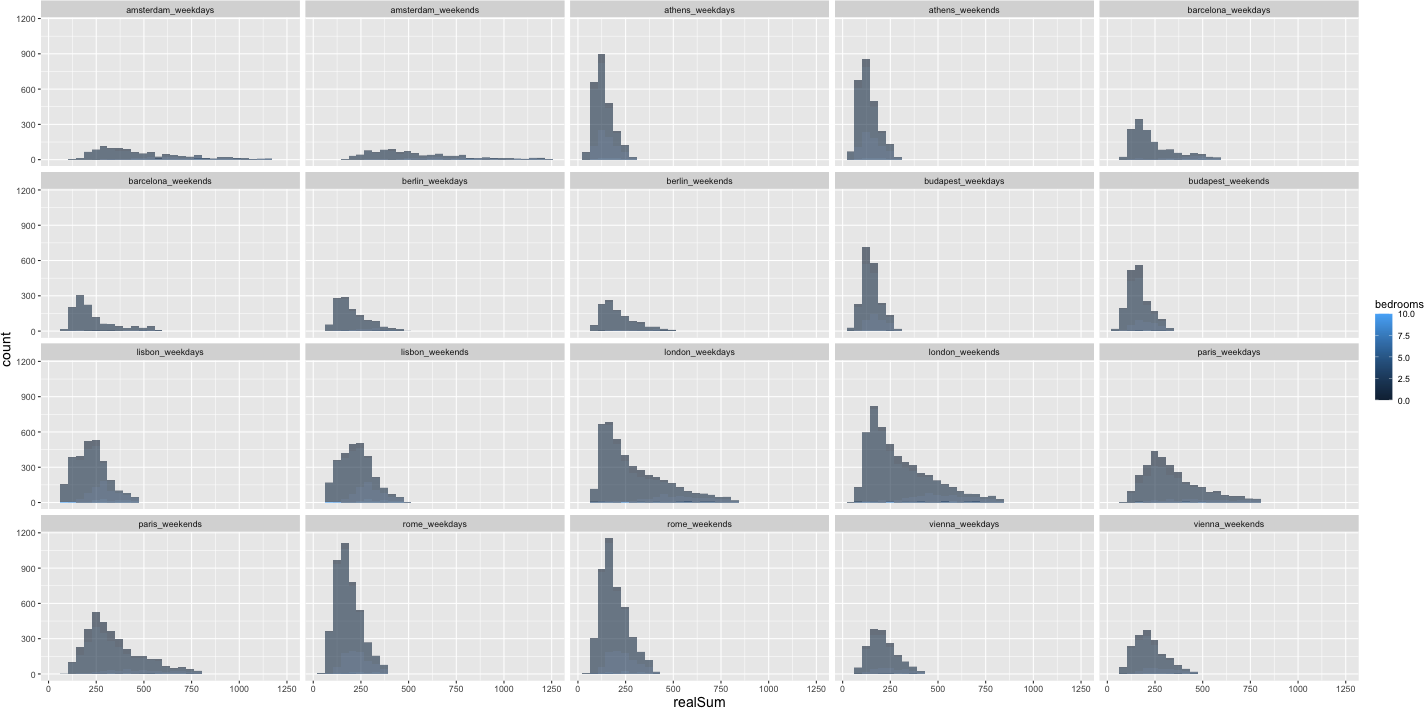
\includegraphics{Project_files/figure-latex/unnamed-chunk-25-3.png}

\begin{Shaded}
\begin{Highlighting}[]
\FunctionTok{ggplot}\NormalTok{(my\_data\_filtered, }\FunctionTok{aes}\NormalTok{(}\AttributeTok{x =} \FunctionTok{reorder}\NormalTok{(city\_day, bedrooms,}
    \AttributeTok{FUN =}\NormalTok{ median), }\AttributeTok{y =}\NormalTok{ bedrooms, }\AttributeTok{fill =}\NormalTok{ city\_day)) }\SpecialCharTok{+} \FunctionTok{geom\_boxplot}\NormalTok{() }\SpecialCharTok{+}
    \FunctionTok{coord\_flip}\NormalTok{() }\SpecialCharTok{+} \FunctionTok{theme}\NormalTok{(}\AttributeTok{legend.key.height =} \FunctionTok{unit}\NormalTok{(}\FloatTok{0.5}\NormalTok{, }\StringTok{"cm"}\NormalTok{),}
    \AttributeTok{legend.key.size =} \FunctionTok{unit}\NormalTok{(}\DecValTok{1}\NormalTok{, }\StringTok{"lines"}\NormalTok{))}
\end{Highlighting}
\end{Shaded}

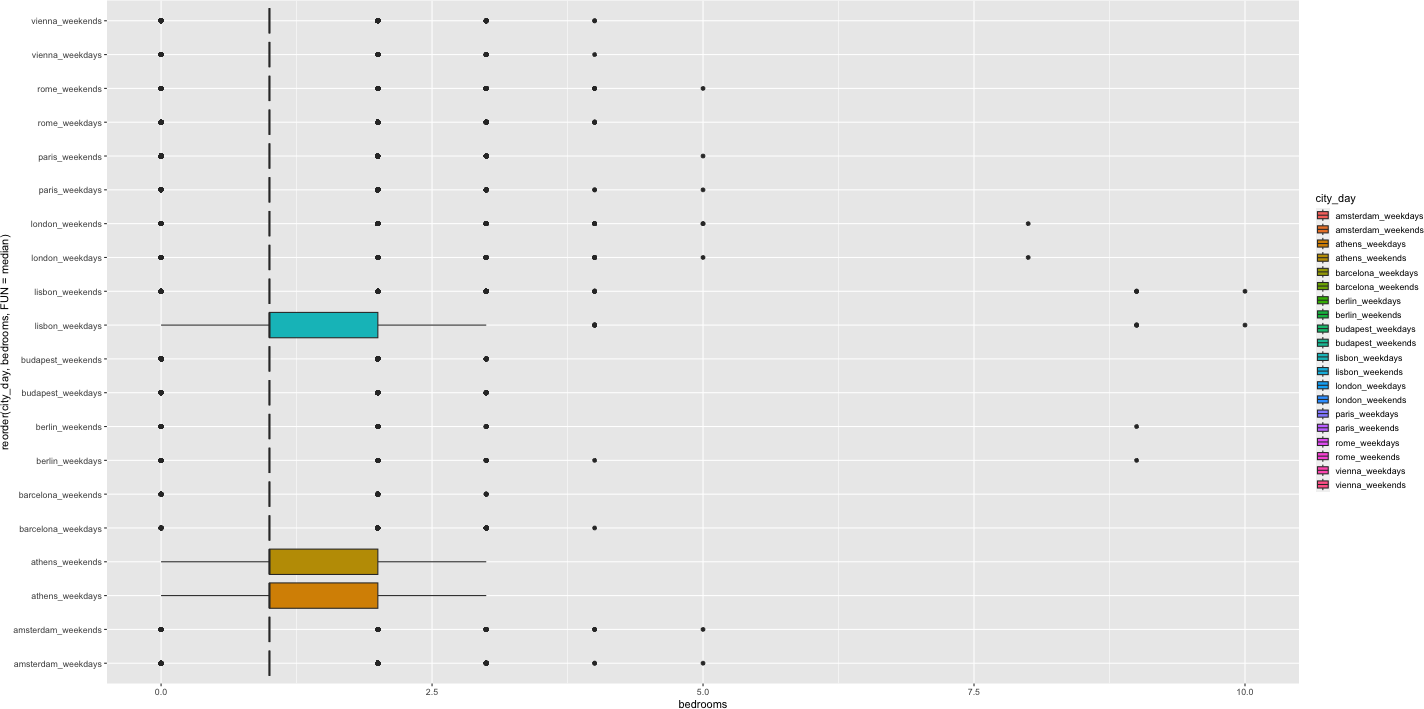
\includegraphics{Project_files/figure-latex/unnamed-chunk-26-1.png}

\begin{Shaded}
\begin{Highlighting}[]
\FunctionTok{cor}\NormalTok{(}\FunctionTok{as.numeric}\NormalTok{(}\FunctionTok{factor}\NormalTok{(my\_data}\SpecialCharTok{$}\NormalTok{multi)), }\FunctionTok{as.numeric}\NormalTok{(}\FunctionTok{factor}\NormalTok{(my\_data}\SpecialCharTok{$}\NormalTok{biz)))}
\end{Highlighting}
\end{Shaded}

\begin{verbatim}
## [1] -0.4707248
\end{verbatim}

\hypertarget{non-outlier-analysis}{%
\subsection{Non Outlier Analysis}\label{non-outlier-analysis}}

\hypertarget{boxplot-of-price-vs-city}{%
\subsubsection{Boxplot of Price Vs
City}\label{boxplot-of-price-vs-city}}

\begin{Shaded}
\begin{Highlighting}[]
\FunctionTok{ggplot}\NormalTok{(my\_data\_filtered, }\FunctionTok{aes}\NormalTok{(}\AttributeTok{x =} \FunctionTok{reorder}\NormalTok{(city\_day, realSum, }\AttributeTok{FUN =}\NormalTok{ median),}
    \AttributeTok{y =}\NormalTok{ realSum, }\AttributeTok{fill =}\NormalTok{ city\_day)) }\SpecialCharTok{+} \FunctionTok{geom\_boxplot}\NormalTok{() }\SpecialCharTok{+} \FunctionTok{coord\_flip}\NormalTok{() }\SpecialCharTok{+}
    \FunctionTok{theme}\NormalTok{(}\AttributeTok{legend.key.height =} \FunctionTok{unit}\NormalTok{(}\FloatTok{0.5}\NormalTok{, }\StringTok{"cm"}\NormalTok{), }\AttributeTok{legend.key.size =} \FunctionTok{unit}\NormalTok{(}\DecValTok{1}\NormalTok{,}
        \StringTok{"lines"}\NormalTok{))}
\end{Highlighting}
\end{Shaded}

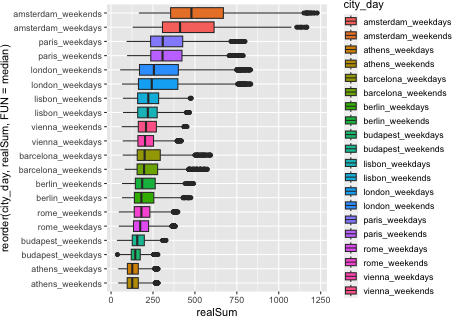
\includegraphics{Project_files/figure-latex/unnamed-chunk-28-1.png}

The highest prices in Europe are found in Amsterdam.

\hypertarget{density-plot-of-price-vs-room-type}{%
\subsubsection{Density plot of Price vs Room
type}\label{density-plot-of-price-vs-room-type}}

\begin{Shaded}
\begin{Highlighting}[]
\FunctionTok{ggplot}\NormalTok{(my\_data\_filtered, }\FunctionTok{aes}\NormalTok{(}\AttributeTok{x =}\NormalTok{ realSum, }\AttributeTok{group =}\NormalTok{ room\_type,}
    \AttributeTok{fill =}\NormalTok{ room\_type, }\AttributeTok{alpha =} \FloatTok{0.2}\NormalTok{)) }\SpecialCharTok{+} \FunctionTok{geom\_density}\NormalTok{()}
\end{Highlighting}
\end{Shaded}

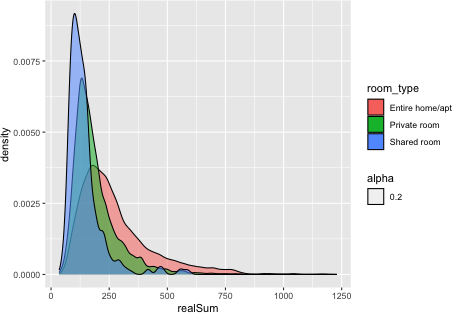
\includegraphics{Project_files/figure-latex/unnamed-chunk-29-1.png}

The prices of entire home are high comparatively

\hypertarget{scatterplot-of-prices-in-rome-w.r.t-latitude-and-longitude-during-weekdays}{%
\subsubsection{Scatterplot of Prices in Rome w.r.t Latitude and
Longitude during
weekdays}\label{scatterplot-of-prices-in-rome-w.r.t-latitude-and-longitude-during-weekdays}}

\begin{Shaded}
\begin{Highlighting}[]
\NormalTok{tema }\OtherTok{\textless{}{-}} \FunctionTok{theme}\NormalTok{(}\AttributeTok{plot.title =} \FunctionTok{element\_text}\NormalTok{(}\AttributeTok{size =} \DecValTok{23}\NormalTok{, }\AttributeTok{hjust =} \FloatTok{0.5}\NormalTok{),}
    \AttributeTok{axis.text.x =} \FunctionTok{element\_text}\NormalTok{(}\AttributeTok{size =} \DecValTok{19}\NormalTok{, }\AttributeTok{face =} \StringTok{"bold"}\NormalTok{), }\AttributeTok{axis.text.y =} \FunctionTok{element\_text}\NormalTok{(}\AttributeTok{size =} \DecValTok{19}\NormalTok{,}
        \AttributeTok{face =} \StringTok{"bold"}\NormalTok{), }\AttributeTok{axis.title.x =} \FunctionTok{element\_text}\NormalTok{(}\AttributeTok{size =} \DecValTok{19}\NormalTok{),}
    \AttributeTok{axis.title.y =} \FunctionTok{element\_text}\NormalTok{(}\AttributeTok{size =} \DecValTok{19}\NormalTok{), }\AttributeTok{legend.text =} \FunctionTok{element\_text}\NormalTok{(}\AttributeTok{colour =} \StringTok{"black"}\NormalTok{,}
        \AttributeTok{size =} \DecValTok{19}\NormalTok{, }\AttributeTok{face =} \StringTok{"bold"}\NormalTok{), }\AttributeTok{legend.background =} \FunctionTok{element\_rect}\NormalTok{(}\AttributeTok{fill =} \StringTok{"\#F5FFFA"}\NormalTok{,}
        \AttributeTok{size =} \FloatTok{0.5}\NormalTok{, }\AttributeTok{linetype =} \StringTok{"dashed"}\NormalTok{, }\AttributeTok{colour =} \StringTok{"black"}\NormalTok{))}

\NormalTok{rome\_data }\OtherTok{\textless{}{-}}\NormalTok{ my\_data\_filtered }\SpecialCharTok{\%\textgreater{}\%}
    \FunctionTok{subset}\NormalTok{(city\_day }\SpecialCharTok{==} \StringTok{"rome\_weekdays"}\NormalTok{)}

\FunctionTok{ggplot}\NormalTok{(}\AttributeTok{data =}\NormalTok{ rome\_data, }\AttributeTok{mapping =} \FunctionTok{aes}\NormalTok{(}\AttributeTok{x =}\NormalTok{ lat, }\AttributeTok{y =}\NormalTok{ lng)) }\SpecialCharTok{+} \FunctionTok{theme\_minimal}\NormalTok{() }\SpecialCharTok{+}
    \FunctionTok{scale\_fill\_identity}\NormalTok{() }\SpecialCharTok{+} \FunctionTok{geom\_point}\NormalTok{(}\AttributeTok{mapping =} \FunctionTok{aes}\NormalTok{(}\AttributeTok{color =}\NormalTok{ realSum),}
    \AttributeTok{size =} \DecValTok{3}\NormalTok{) }\SpecialCharTok{+} \FunctionTok{ggtitle}\NormalTok{(}\StringTok{""}\NormalTok{) }\SpecialCharTok{+}\NormalTok{ tema}
\end{Highlighting}
\end{Shaded}

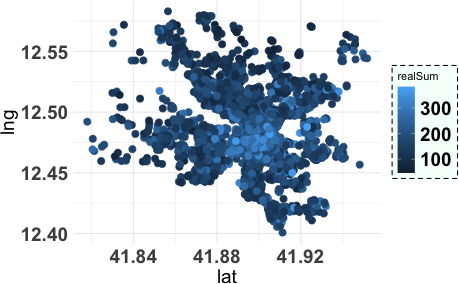
\includegraphics{Project_files/figure-latex/unnamed-chunk-30-1.png}

This plot is within expectations of general trends, which suggests
similar types of establishments (price and hospitality) tend be in
clusters.

\hypertarget{different-model-selection-and-training}{%
\section{Different Model Selection and
Training}\label{different-model-selection-and-training}}

\hypertarget{checking-for-correlations-between-different-attributes}{%
\subsection{Checking for correlations between different
attributes}\label{checking-for-correlations-between-different-attributes}}

\begin{Shaded}
\begin{Highlighting}[]
\FunctionTok{ggpairs}\NormalTok{(my\_data[}\FunctionTok{c}\NormalTok{(}\StringTok{"realSum"}\NormalTok{, }\StringTok{"dist"}\NormalTok{, }\StringTok{"metro\_dist"}\NormalTok{, }\StringTok{"attr\_index\_norm"}\NormalTok{,}
    \StringTok{"rest\_index\_norm"}\NormalTok{, }\StringTok{"city\_day"}\NormalTok{)], }\AttributeTok{cardinality =} \DecValTok{20}\NormalTok{, }\AttributeTok{cardinality\_threshold =} \DecValTok{999}\NormalTok{)}
\end{Highlighting}
\end{Shaded}

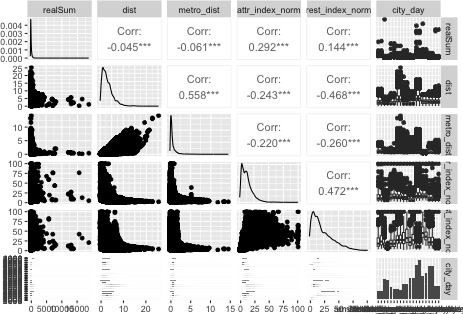
\includegraphics{Project_files/figure-latex/unnamed-chunk-31-1.png}

\begin{Shaded}
\begin{Highlighting}[]
\FunctionTok{ggpairs}\NormalTok{(my\_data\_filtered[}\FunctionTok{c}\NormalTok{(}\StringTok{"realSum"}\NormalTok{, }\StringTok{"dist"}\NormalTok{, }\StringTok{"metro\_dist"}\NormalTok{, }\StringTok{"attr\_index\_norm"}\NormalTok{,}
    \StringTok{"rest\_index\_norm"}\NormalTok{, }\StringTok{"city\_day"}\NormalTok{)], }\AttributeTok{cardinality =} \DecValTok{20}\NormalTok{, }\AttributeTok{cardinality\_threshold =} \DecValTok{999}\NormalTok{)}
\end{Highlighting}
\end{Shaded}

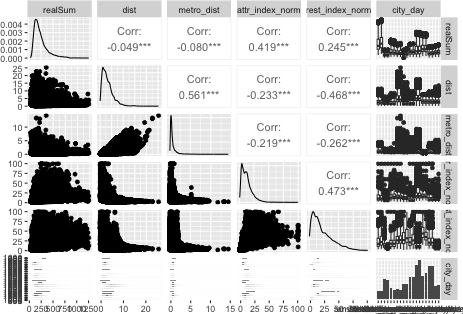
\includegraphics{Project_files/figure-latex/unnamed-chunk-32-1.png}

\begin{Shaded}
\begin{Highlighting}[]
\FunctionTok{cor}\NormalTok{(my\_data}\SpecialCharTok{$}\NormalTok{attr\_index, my\_data}\SpecialCharTok{$}\NormalTok{rest\_index)}
\end{Highlighting}
\end{Shaded}

\begin{verbatim}
## [1] 0.4721427
\end{verbatim}

\begin{Shaded}
\begin{Highlighting}[]
\FunctionTok{ggplot}\NormalTok{() }\SpecialCharTok{+} \FunctionTok{geom\_point}\NormalTok{(}\AttributeTok{data =}\NormalTok{ my\_data\_filtered, }\FunctionTok{aes}\NormalTok{(}\AttributeTok{x =}\NormalTok{ attr\_index\_norm,}
    \AttributeTok{y =}\NormalTok{ rest\_index\_norm, }\AttributeTok{color =} \StringTok{"Filtered Data"}\NormalTok{), }\AttributeTok{alpha =} \FloatTok{0.4}\NormalTok{) }\SpecialCharTok{+}
    \FunctionTok{geom\_point}\NormalTok{(}\AttributeTok{data =}\NormalTok{ my\_outliers, }\FunctionTok{aes}\NormalTok{(}\AttributeTok{x =}\NormalTok{ attr\_index\_norm, }\AttributeTok{y =}\NormalTok{ rest\_index\_norm,}
        \AttributeTok{color =} \StringTok{"Outliers"}\NormalTok{), }\AttributeTok{alpha =} \FloatTok{0.4}\NormalTok{) }\SpecialCharTok{+} \FunctionTok{scale\_color\_manual}\NormalTok{(}\AttributeTok{values =} \FunctionTok{c}\NormalTok{(}\StringTok{\textasciigrave{}}\AttributeTok{Filtered Data}\StringTok{\textasciigrave{}} \OtherTok{=} \StringTok{"blue"}\NormalTok{,}
    \AttributeTok{Outliers =} \StringTok{"red"}\NormalTok{))}
\end{Highlighting}
\end{Shaded}

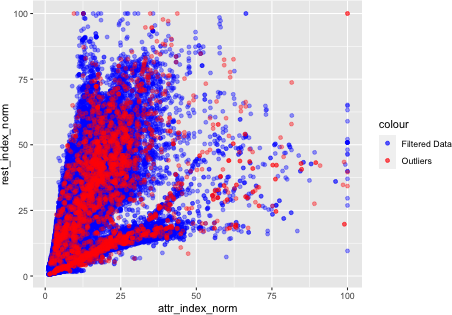
\includegraphics{Project_files/figure-latex/unnamed-chunk-34-1.png}

\begin{Shaded}
\begin{Highlighting}[]
\FunctionTok{ggplot}\NormalTok{() }\SpecialCharTok{+} \FunctionTok{geom\_point}\NormalTok{(}\AttributeTok{data =}\NormalTok{ my\_data\_filtered, }\FunctionTok{aes}\NormalTok{(}\AttributeTok{x =}\NormalTok{ attr\_index\_norm,}
    \AttributeTok{y =}\NormalTok{ rest\_index\_norm, }\AttributeTok{color =} \StringTok{"Filtered Data"}\NormalTok{), }\AttributeTok{alpha =} \FloatTok{0.4}\NormalTok{) }\SpecialCharTok{+}
    \FunctionTok{geom\_point}\NormalTok{(}\AttributeTok{data =}\NormalTok{ my\_outliers, }\FunctionTok{aes}\NormalTok{(}\AttributeTok{x =}\NormalTok{ attr\_index\_norm, }\AttributeTok{y =}\NormalTok{ rest\_index\_norm,}
        \AttributeTok{color =} \StringTok{"Outliers"}\NormalTok{), }\AttributeTok{alpha =} \FloatTok{0.4}\NormalTok{) }\SpecialCharTok{+} \FunctionTok{scale\_color\_manual}\NormalTok{(}\AttributeTok{values =} \FunctionTok{c}\NormalTok{(}\StringTok{\textasciigrave{}}\AttributeTok{Filtered Data}\StringTok{\textasciigrave{}} \OtherTok{=} \StringTok{"blue"}\NormalTok{,}
    \AttributeTok{Outliers =} \StringTok{"red"}\NormalTok{)) }\SpecialCharTok{+} \FunctionTok{facet\_wrap}\NormalTok{(}\SpecialCharTok{\textasciitilde{}}\NormalTok{city\_day)}
\end{Highlighting}
\end{Shaded}

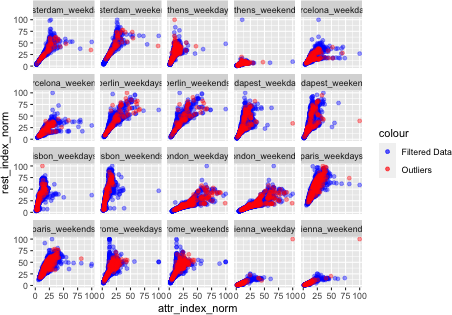
\includegraphics{Project_files/figure-latex/unnamed-chunk-34-2.png}

\begin{Shaded}
\begin{Highlighting}[]
\FunctionTok{ggplot}\NormalTok{() }\SpecialCharTok{+} \FunctionTok{geom\_point}\NormalTok{(}\AttributeTok{data =}\NormalTok{ my\_data, }\FunctionTok{aes}\NormalTok{(}\AttributeTok{x =}\NormalTok{ attr\_index\_norm,}
    \AttributeTok{y =}\NormalTok{ rest\_index\_norm, }\AttributeTok{color =} \StringTok{"Filtered Data"}\NormalTok{), }\AttributeTok{alpha =} \FloatTok{0.4}\NormalTok{) }\SpecialCharTok{+}
    \FunctionTok{scale\_color\_manual}\NormalTok{(}\AttributeTok{values =} \FunctionTok{c}\NormalTok{(}\StringTok{\textasciigrave{}}\AttributeTok{Filtered Data}\StringTok{\textasciigrave{}} \OtherTok{=} \StringTok{"blue"}\NormalTok{))}
\end{Highlighting}
\end{Shaded}

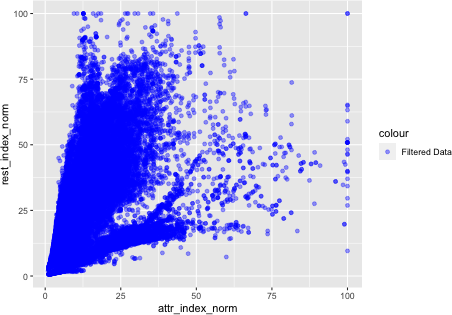
\includegraphics{Project_files/figure-latex/unnamed-chunk-34-3.png}

\begin{Shaded}
\begin{Highlighting}[]
\FunctionTok{ggplot}\NormalTok{() }\SpecialCharTok{+} \FunctionTok{geom\_point}\NormalTok{(}\AttributeTok{data =}\NormalTok{ my\_data, }\FunctionTok{aes}\NormalTok{(}\AttributeTok{x =}\NormalTok{ attr\_index\_norm,}
    \AttributeTok{y =}\NormalTok{ rest\_index\_norm, }\AttributeTok{color =} \StringTok{"Filtered Data"}\NormalTok{), }\AttributeTok{alpha =} \FloatTok{0.4}\NormalTok{) }\SpecialCharTok{+}
    \FunctionTok{scale\_color\_manual}\NormalTok{(}\AttributeTok{values =} \FunctionTok{c}\NormalTok{(}\StringTok{\textasciigrave{}}\AttributeTok{Filtered Data}\StringTok{\textasciigrave{}} \OtherTok{=} \StringTok{"blue"}\NormalTok{)) }\SpecialCharTok{+}
    \FunctionTok{facet\_wrap}\NormalTok{(}\SpecialCharTok{\textasciitilde{}}\NormalTok{city\_day)}
\end{Highlighting}
\end{Shaded}

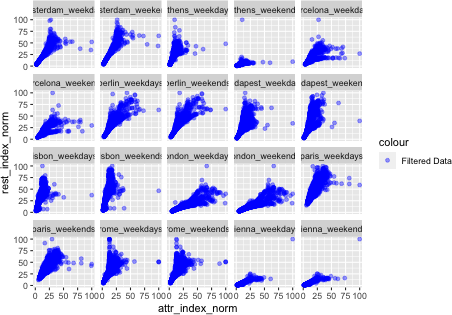
\includegraphics{Project_files/figure-latex/unnamed-chunk-34-4.png}

\begin{Shaded}
\begin{Highlighting}[]
\FunctionTok{cor}\NormalTok{(my\_data}\SpecialCharTok{$}\NormalTok{attr\_index\_norm, my\_data}\SpecialCharTok{$}\NormalTok{rest\_index\_norm)}
\end{Highlighting}
\end{Shaded}

\begin{verbatim}
## [1] 0.4721427
\end{verbatim}

\hypertarget{linear-regression}{%
\subsection{Linear Regression}\label{linear-regression}}

\begin{Shaded}
\begin{Highlighting}[]
\NormalTok{M1 }\OtherTok{\textless{}{-}} \FunctionTok{lm}\NormalTok{(realSum }\SpecialCharTok{\textasciitilde{}}\NormalTok{ . }\SpecialCharTok{{-}}\NormalTok{ realSum, }\AttributeTok{data =}\NormalTok{ my\_data\_train)}
\FunctionTok{summary}\NormalTok{(M1)}
\end{Highlighting}
\end{Shaded}

\begin{verbatim}
## 
## Call:
## lm(formula = realSum ~ . - realSum, data = my_data_train)
## 
## Residuals:
##     Min      1Q  Median      3Q     Max 
##  -757.5   -84.1   -21.0    43.0 18422.1 
## 
## Coefficients:
##                              Estimate Std. Error t value Pr(>|t|)    
## (Intercept)                -4.916e+03  3.997e+03  -1.230 0.218657    
## X                           1.026e-03  1.605e-03   0.639 0.522652    
## room_typePrivate room      -1.144e+02  4.282e+00 -26.703  < 2e-16 ***
## room_typeShared room       -2.043e+02  1.894e+01 -10.790  < 2e-16 ***
## person_capacity             2.396e+01  1.765e+00  13.578  < 2e-16 ***
## host_is_superhostTrue       1.152e+00  3.936e+00   0.293 0.769759    
## multi                       9.638e+00  4.133e+00   2.332 0.019704 *  
## biz                         3.332e+01  4.189e+00   7.954 1.85e-15 ***
## cleanliness_rating          5.045e+00  2.415e+00   2.089 0.036740 *  
## guest_satisfaction_overall  7.759e-01  2.615e-01   2.968 0.003003 ** 
## bedrooms                    8.599e+01  3.189e+00  26.965  < 2e-16 ***
## dist                       -1.538e+00  1.263e+00  -1.218 0.223192    
## metro_dist                 -3.879e+00  2.509e+00  -1.546 0.122147    
## attr_index_norm             6.375e+00  2.946e-01  21.636  < 2e-16 ***
## rest_index_norm            -1.736e-01  1.781e-01  -0.975 0.329728    
## lng                        -2.619e+02  4.023e+01  -6.510 7.63e-11 ***
## lat                         1.224e+02  7.653e+01   1.599 0.109884    
## city_dayamsterdam_weekends  6.796e+01  1.600e+01   4.247 2.17e-05 ***
## city_dayathens_weekdays     6.283e+03  1.389e+03   4.522 6.15e-06 ***
## city_dayathens_weekends     6.271e+03  1.390e+03   4.513 6.41e-06 ***
## city_daybarcelona_weekdays  4.051e+02  8.379e+02   0.483 0.628751    
## city_daybarcelona_weekends  4.231e+02  8.379e+02   0.505 0.613579    
## city_dayberlin_weekdays     1.940e+03  3.424e+02   5.666 1.47e-08 ***
## city_dayberlin_weekends     1.950e+03  3.423e+02   5.697 1.23e-08 ***
## city_daybudapest_weekdays   3.883e+03  7.075e+02   5.488 4.09e-08 ***
## city_daybudapest_weekends   3.910e+03  7.075e+02   5.527 3.28e-08 ***
## city_daylisbon_weekdays    -2.311e+03  1.144e+03  -2.020 0.043372 *  
## city_daylisbon_weekends    -2.302e+03  1.144e+03  -2.013 0.044164 *  
## city_daylondon_weekdays    -1.407e+03  2.062e+02  -6.823 9.06e-12 ***
## city_daylondon_weekends    -1.409e+03  2.062e+02  -6.833 8.47e-12 ***
## city_dayparis_weekdays     -4.046e+02  2.785e+02  -1.453 0.146310    
## city_dayparis_weekends     -4.238e+02  2.787e+02  -1.521 0.128294    
## city_dayrome_weekdays       2.929e+03  8.819e+02   3.322 0.000896 ***
## city_dayrome_weekends       2.934e+03  8.819e+02   3.327 0.000879 ***
## city_dayvienna_weekdays     3.216e+03  5.832e+02   5.515 3.51e-08 ***
## city_dayvienna_weekends     3.215e+03  5.833e+02   5.511 3.59e-08 ***
## ---
## Signif. codes:  0 '***' 0.001 '**' 0.01 '*' 0.05 '.' 0.1 ' ' 1
## 
## Residual standard error: 305.1 on 36158 degrees of freedom
## Multiple R-squared:  0.2151, Adjusted R-squared:  0.2143 
## F-statistic:   283 on 35 and 36158 DF,  p-value: < 2.2e-16
\end{verbatim}

The r\^{}2 and adjusted r\^{}2 values are too low for the Linear
regression model to be considered a competent one in this case.

\hypertarget{lasso-step-regression}{%
\subsection{Lasso Step Regression}\label{lasso-step-regression}}

\begin{Shaded}
\begin{Highlighting}[]
\NormalTok{M1\_step }\OtherTok{=} \FunctionTok{step}\NormalTok{(M1, }\AttributeTok{direction =} \StringTok{"backward"}\NormalTok{)}
\end{Highlighting}
\end{Shaded}

\begin{verbatim}
## Start:  AIC=414133.9
## realSum ~ (X + room_type + person_capacity + host_is_superhost + 
##     multi + biz + cleanliness_rating + guest_satisfaction_overall + 
##     bedrooms + dist + metro_dist + attr_index_norm + rest_index_norm + 
##     lng + lat + city_day) - realSum
## 
##                              Df Sum of Sq        RSS    AIC
## - host_is_superhost           1      7973 3365094746 414132
## - X                           1     38033 3365124806 414132
## - rest_index_norm             1     88412 3365175185 414133
## - dist                        1    138090 3365224863 414133
## <none>                                    3365086773 414134
## - metro_dist                  1    222399 3365309172 414134
## - lat                         1    237878 3365324651 414134
## - cleanliness_rating          1    406023 3365492796 414136
## - multi                       1    506134 3365592907 414137
## - guest_satisfaction_overall  1    819629 3365906402 414141
## - lng                         1   3943764 3369030537 414174
## - biz                         1   5888249 3370975022 414195
## - person_capacity             1  17158129 3382244902 414316
## - attr_index_norm             1  43565736 3408652509 414598
## - bedrooms                    1  67668883 3432755656 414853
## - room_type                   2  74087785 3439174558 414918
## - city_day                   19 129073720 3494160493 415458
## 
## Step:  AIC=414132
## realSum ~ X + room_type + person_capacity + multi + biz + cleanliness_rating + 
##     guest_satisfaction_overall + bedrooms + dist + metro_dist + 
##     attr_index_norm + rest_index_norm + lng + lat + city_day
## 
##                              Df Sum of Sq        RSS    AIC
## - X                           1     37006 3365131752 414130
## - rest_index_norm             1     87739 3365182485 414131
## - dist                        1    137403 3365232149 414131
## <none>                                    3365094746 414132
## - metro_dist                  1    224011 3365318757 414132
## - lat                         1    236846 3365331592 414133
## - cleanliness_rating          1    422853 3365517599 414135
## - multi                       1    513494 3365608240 414136
## - guest_satisfaction_overall  1    846062 3365940808 414139
## - lng                         1   3943452 3369038198 414172
## - biz                         1   5880284 3370975030 414193
## - person_capacity             1  17156242 3382250987 414314
## - attr_index_norm             1  43564593 3408659339 414596
## - bedrooms                    1  67662885 3432757630 414851
## - room_type                   2  74127027 3439221773 414917
## - city_day                   19 129091002 3494185748 415457
## 
## Step:  AIC=414130.4
## realSum ~ room_type + person_capacity + multi + biz + cleanliness_rating + 
##     guest_satisfaction_overall + bedrooms + dist + metro_dist + 
##     attr_index_norm + rest_index_norm + lng + lat + city_day
## 
##                              Df Sum of Sq        RSS    AIC
## - rest_index_norm             1     99078 3365230830 414129
## - dist                        1    136528 3365268280 414130
## <none>                                    3365131752 414130
## - metro_dist                  1    238734 3365370486 414131
## - lat                         1    240263 3365372016 414131
## - cleanliness_rating          1    420972 3365552724 414133
## - multi                       1    509297 3365641049 414134
## - guest_satisfaction_overall  1    845143 3365976896 414138
## - lng                         1   3980694 3369112446 414171
## - biz                         1   5868776 3371000528 414191
## - person_capacity             1  17162129 3382293881 414313
## - attr_index_norm             1  43529070 3408660822 414594
## - bedrooms                    1  67709766 3432841518 414849
## - room_type                   2  74127155 3439258907 414915
## - city_day                   19 130900670 3496032422 415474
## 
## Step:  AIC=414129.5
## realSum ~ room_type + person_capacity + multi + biz + cleanliness_rating + 
##     guest_satisfaction_overall + bedrooms + dist + metro_dist + 
##     attr_index_norm + lng + lat + city_day
## 
##                              Df Sum of Sq        RSS    AIC
## - dist                        1     86683 3365317513 414128
## <none>                                    3365230830 414129
## - metro_dist                  1    272120 3365502950 414130
## - lat                         1    273162 3365503992 414130
## - cleanliness_rating          1    419524 3365650354 414132
## - multi                       1    494022 3365724852 414133
## - guest_satisfaction_overall  1    837305 3366068136 414136
## - lng                         1   3973420 3369204250 414170
## - biz                         1   5789568 3371020398 414190
## - person_capacity             1  17121733 3382352564 414311
## - attr_index_norm             1  54609498 3419840328 414710
## - bedrooms                    1  67904086 3433134916 414851
## - room_type                   2  74039649 3439270479 414913
## - city_day                   19 131071208 3496302038 415474
## 
## Step:  AIC=414128.4
## realSum ~ room_type + person_capacity + multi + biz + cleanliness_rating + 
##     guest_satisfaction_overall + bedrooms + metro_dist + attr_index_norm + 
##     lng + lat + city_day
## 
##                              Df Sum of Sq        RSS    AIC
## <none>                                    3365317513 414128
## - lat                         1    292396 3365609909 414130
## - cleanliness_rating          1    414092 3365731605 414131
## - multi                       1    495582 3365813095 414132
## - metro_dist                  1    614735 3365932248 414133
## - guest_satisfaction_overall  1    838098 3366155612 414135
## - lng                         1   3887405 3369204918 414168
## - biz                         1   5842686 3371160199 414189
## - person_capacity             1  17112579 3382430092 414310
## - bedrooms                    1  67830738 3433148251 414849
## - room_type                   2  74300129 3439617642 414915
## - attr_index_norm             1  86947824 3452265337 415050
## - city_day                   19 133905560 3499223073 415503
\end{verbatim}

\begin{Shaded}
\begin{Highlighting}[]
\FunctionTok{summary}\NormalTok{(M1\_step)}
\end{Highlighting}
\end{Shaded}

\begin{verbatim}
## 
## Call:
## lm(formula = realSum ~ room_type + person_capacity + multi + 
##     biz + cleanliness_rating + guest_satisfaction_overall + bedrooms + 
##     metro_dist + attr_index_norm + lng + lat + city_day, data = my_data_train)
## 
## Residuals:
##     Min      1Q  Median      3Q     Max 
##  -756.8   -84.1   -21.0    42.9 18422.9 
## 
## Coefficients:
##                              Estimate Std. Error t value Pr(>|t|)    
## (Intercept)                -5594.6616  3968.4120  -1.410 0.158608    
## room_typePrivate room       -114.3509     4.2751 -26.748  < 2e-16 ***
## room_typeShared room        -203.5745    18.9242 -10.757  < 2e-16 ***
## person_capacity               23.9228     1.7642  13.560  < 2e-16 ***
## multi                          9.5185     4.1248   2.308 0.021024 *  
## biz                           33.0599     4.1724   7.924 2.37e-15 ***
## cleanliness_rating             5.0657     2.4015   2.109 0.034916 *  
## guest_satisfaction_overall     0.7802     0.2600   3.001 0.002693 ** 
## bedrooms                      86.0342     3.1867  26.998  < 2e-16 ***
## metro_dist                    -5.4925     2.1370  -2.570 0.010170 *  
## attr_index_norm                6.3667     0.2083  30.566  < 2e-16 ***
## lng                         -257.3918    39.8246  -6.463 1.04e-10 ***
## lat                          134.7768    76.0355   1.773 0.076312 .  
## city_dayamsterdam_weekends    67.1363    15.9781   4.202 2.65e-05 ***
## city_dayathens_weekdays     6380.0626  1384.2639   4.609 4.06e-06 ***
## city_dayathens_weekends     6370.9186  1384.2104   4.603 4.19e-06 ***
## city_daybarcelona_weekdays   554.5173   831.2840   0.667 0.504737    
## city_daybarcelona_weekends   572.4049   831.2994   0.689 0.491101    
## city_dayberlin_weekdays     1895.1920   338.3471   5.601 2.14e-08 ***
## city_dayberlin_weekends     1904.8977   338.2674   5.631 1.80e-08 ***
## city_daybudapest_weekdays   3880.0408   704.0633   5.511 3.59e-08 ***
## city_daybudapest_weekends   3906.3502   704.0708   5.548 2.91e-08 ***
## city_daylisbon_weekdays    -2077.4612  1130.8273  -1.837 0.066201 .  
## city_daylisbon_weekends    -2069.6484  1130.8363  -1.830 0.067229 .  
## city_daylondon_weekdays    -1373.5039   204.1097  -6.729 1.73e-11 ***
## city_daylondon_weekends    -1375.1043   204.1230  -6.737 1.65e-11 ***
## city_dayparis_weekdays      -354.6025   276.2027  -1.284 0.199203    
## city_dayparis_weekends      -371.8162   276.2127  -1.346 0.178271    
## city_dayrome_weekdays       3026.1639   878.2040   3.446 0.000570 ***
## city_dayrome_weekends       3031.0164   878.2293   3.451 0.000559 ***
## city_dayvienna_weekdays     3219.2260   580.2311   5.548 2.91e-08 ***
## city_dayvienna_weekends     3217.6304   580.3196   5.545 2.97e-08 ***
## ---
## Signif. codes:  0 '***' 0.001 '**' 0.01 '*' 0.05 '.' 0.1 ' ' 1
## 
## Residual standard error: 305.1 on 36162 degrees of freedom
## Multiple R-squared:  0.215,  Adjusted R-squared:  0.2143 
## F-statistic: 319.5 on 31 and 36162 DF,  p-value: < 2.2e-16
\end{verbatim}

The stepwise regression removed - host\_is\_superhost,
rest\_index\_norm, dist

\begin{Shaded}
\begin{Highlighting}[]
\NormalTok{lm\_pred }\OtherTok{\textless{}{-}} \FunctionTok{predict}\NormalTok{(M1\_step, }\AttributeTok{newdata =}\NormalTok{ my\_data\_test)}
\NormalTok{y\_test }\OtherTok{\textless{}{-}}\NormalTok{ my\_data\_test}\SpecialCharTok{$}\NormalTok{realSum}

\NormalTok{RMSE }\OtherTok{=} \FunctionTok{sqrt}\NormalTok{(}\FunctionTok{mean}\NormalTok{((y\_test }\SpecialCharTok{{-}}\NormalTok{ lm\_pred)}\SpecialCharTok{\^{}}\DecValTok{2}\NormalTok{))}
\NormalTok{RMSE}
\end{Highlighting}
\end{Shaded}

\begin{verbatim}
## [1] 233.2787
\end{verbatim}

\begin{Shaded}
\begin{Highlighting}[]
\CommentTok{\# Prepare the predictors and response variable}
\NormalTok{x\_train }\OtherTok{\textless{}{-}} \FunctionTok{model.matrix}\NormalTok{(realSum }\SpecialCharTok{\textasciitilde{}}\NormalTok{ room\_type }\SpecialCharTok{+}\NormalTok{ person\_capacity }\SpecialCharTok{+}
\NormalTok{    host\_is\_superhost }\SpecialCharTok{+}\NormalTok{ multi }\SpecialCharTok{+}\NormalTok{ biz }\SpecialCharTok{+}\NormalTok{ cleanliness\_rating }\SpecialCharTok{+}\NormalTok{ guest\_satisfaction\_overall }\SpecialCharTok{+}
\NormalTok{    bedrooms }\SpecialCharTok{+}\NormalTok{ dist }\SpecialCharTok{+}\NormalTok{ metro\_dist }\SpecialCharTok{+}\NormalTok{ attr\_index\_norm }\SpecialCharTok{+}\NormalTok{ rest\_index\_norm }\SpecialCharTok{+}
\NormalTok{    lng }\SpecialCharTok{+}\NormalTok{ lat }\SpecialCharTok{+}\NormalTok{ city\_day, }\AttributeTok{data =}\NormalTok{ my\_data\_train)[, }\SpecialCharTok{{-}}\DecValTok{1}\NormalTok{]}
\NormalTok{y\_train }\OtherTok{\textless{}{-}}\NormalTok{ my\_data\_train}\SpecialCharTok{$}\NormalTok{realSum}

\CommentTok{\# Fit a Lasso regression model}
\NormalTok{lasso\_model }\OtherTok{\textless{}{-}} \FunctionTok{glmnet}\NormalTok{(x\_train, y\_train, }\AttributeTok{alpha =} \DecValTok{1}\NormalTok{)}

\CommentTok{\# Select the best lambda value using cross{-}validation}
\NormalTok{cv\_model }\OtherTok{\textless{}{-}} \FunctionTok{cv.glmnet}\NormalTok{(x\_train, y\_train, }\AttributeTok{alpha =} \DecValTok{1}\NormalTok{, }\AttributeTok{nfolds =} \DecValTok{5}\NormalTok{)}

\CommentTok{\# Plot the cross{-}validation results}
\FunctionTok{plot}\NormalTok{(cv\_model)}
\end{Highlighting}
\end{Shaded}

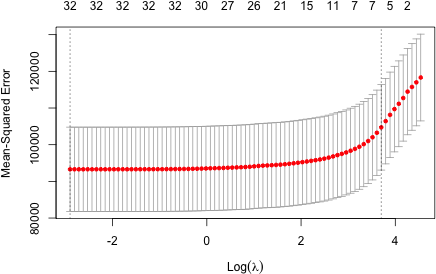
\includegraphics{Project_files/figure-latex/unnamed-chunk-40-1.png}

\begin{Shaded}
\begin{Highlighting}[]
\CommentTok{\# Select the lambda value that minimizes the mean}
\CommentTok{\# cross{-}validation error}
\NormalTok{best\_lambda }\OtherTok{\textless{}{-}}\NormalTok{ cv\_model}\SpecialCharTok{$}\NormalTok{lambda.min}

\CommentTok{\# Fit a Lasso regression model with the selected lambda}
\CommentTok{\# value}
\NormalTok{lasso\_model\_best }\OtherTok{\textless{}{-}} \FunctionTok{glmnet}\NormalTok{(x\_train, y\_train, }\AttributeTok{alpha =} \DecValTok{1}\NormalTok{, }\AttributeTok{lambda =}\NormalTok{ best\_lambda)}

\CommentTok{\# Calculate R{-}squared and multiple R{-}squared}
\NormalTok{y\_train\_pred }\OtherTok{\textless{}{-}} \FunctionTok{predict}\NormalTok{(lasso\_model\_best, }\AttributeTok{newx =}\NormalTok{ x\_train)}
\NormalTok{y\_train\_mean }\OtherTok{\textless{}{-}} \FunctionTok{mean}\NormalTok{(y\_train)}
\NormalTok{SST }\OtherTok{\textless{}{-}} \FunctionTok{sum}\NormalTok{((y\_train }\SpecialCharTok{{-}}\NormalTok{ y\_train\_mean)}\SpecialCharTok{\^{}}\DecValTok{2}\NormalTok{)}
\NormalTok{SSR }\OtherTok{\textless{}{-}} \FunctionTok{sum}\NormalTok{((y\_train }\SpecialCharTok{{-}}\NormalTok{ y\_train\_pred)}\SpecialCharTok{\^{}}\DecValTok{2}\NormalTok{)}
\NormalTok{R\_squared }\OtherTok{\textless{}{-}} \DecValTok{1} \SpecialCharTok{{-}}\NormalTok{ SSR}\SpecialCharTok{/}\NormalTok{SST}
\NormalTok{multiple\_R\_squared }\OtherTok{\textless{}{-}} \FunctionTok{cor}\NormalTok{(y\_train\_pred, y\_train)}\SpecialCharTok{\^{}}\DecValTok{2}
\NormalTok{n }\OtherTok{\textless{}{-}} \FunctionTok{length}\NormalTok{(y\_train)}
\NormalTok{p }\OtherTok{\textless{}{-}} \FunctionTok{ncol}\NormalTok{(x\_train)}
\NormalTok{adj\_R\_squared }\OtherTok{\textless{}{-}} \DecValTok{1} \SpecialCharTok{{-}}\NormalTok{ (SSR}\SpecialCharTok{/}\NormalTok{(n }\SpecialCharTok{{-}}\NormalTok{ p }\SpecialCharTok{{-}} \DecValTok{1}\NormalTok{))}\SpecialCharTok{/}\NormalTok{(SST}\SpecialCharTok{/}\NormalTok{(n }\SpecialCharTok{{-}} \DecValTok{1}\NormalTok{))}


\CommentTok{\# Print the R{-}squared and multiple R{-}squared values}
\FunctionTok{cat}\NormalTok{(}\StringTok{"R{-}squared:"}\NormalTok{, }\FunctionTok{round}\NormalTok{(R\_squared, }\DecValTok{3}\NormalTok{), }\StringTok{"}\SpecialCharTok{\textbackslash{}n}\StringTok{"}\NormalTok{)}
\end{Highlighting}
\end{Shaded}

\begin{verbatim}
## R-squared: 0.214
\end{verbatim}

\begin{Shaded}
\begin{Highlighting}[]
\FunctionTok{cat}\NormalTok{(}\StringTok{"Multiple R{-}squared:"}\NormalTok{, }\FunctionTok{round}\NormalTok{(multiple\_R\_squared, }\DecValTok{3}\NormalTok{), }\StringTok{"}\SpecialCharTok{\textbackslash{}n}\StringTok{"}\NormalTok{)}
\end{Highlighting}
\end{Shaded}

\begin{verbatim}
## Multiple R-squared: 0.214
\end{verbatim}

\begin{Shaded}
\begin{Highlighting}[]
\FunctionTok{cat}\NormalTok{(}\StringTok{"Adjusted R{-}squared:"}\NormalTok{, }\FunctionTok{round}\NormalTok{(adj\_R\_squared, }\DecValTok{3}\NormalTok{), }\StringTok{"}\SpecialCharTok{\textbackslash{}n}\StringTok{"}\NormalTok{)}
\end{Highlighting}
\end{Shaded}

\begin{verbatim}
## Adjusted R-squared: 0.213
\end{verbatim}

\begin{Shaded}
\begin{Highlighting}[]
\CommentTok{\# Predict on the test data}
\NormalTok{x\_test }\OtherTok{\textless{}{-}} \FunctionTok{model.matrix}\NormalTok{(realSum }\SpecialCharTok{\textasciitilde{}}\NormalTok{ room\_type }\SpecialCharTok{+}\NormalTok{ person\_capacity }\SpecialCharTok{+}
\NormalTok{    host\_is\_superhost }\SpecialCharTok{+}\NormalTok{ multi }\SpecialCharTok{+}\NormalTok{ biz }\SpecialCharTok{+}\NormalTok{ cleanliness\_rating }\SpecialCharTok{+}\NormalTok{ guest\_satisfaction\_overall }\SpecialCharTok{+}
\NormalTok{    bedrooms }\SpecialCharTok{+}\NormalTok{ dist }\SpecialCharTok{+}\NormalTok{ metro\_dist }\SpecialCharTok{+}\NormalTok{ attr\_index\_norm }\SpecialCharTok{+}\NormalTok{ rest\_index\_norm }\SpecialCharTok{+}
\NormalTok{    lng }\SpecialCharTok{+}\NormalTok{ lat }\SpecialCharTok{+}\NormalTok{ city\_day, }\AttributeTok{data =}\NormalTok{ my\_data\_test)[, }\SpecialCharTok{{-}}\DecValTok{1}\NormalTok{]}
\NormalTok{y\_test }\OtherTok{\textless{}{-}}\NormalTok{ my\_data\_test}\SpecialCharTok{$}\NormalTok{realSum}
\NormalTok{lasso\_pred }\OtherTok{\textless{}{-}} \FunctionTok{predict}\NormalTok{(lasso\_model\_best, }\AttributeTok{newx =}\NormalTok{ x\_test)}

\CommentTok{\# Evaluate the model performance}
\NormalTok{rmse }\OtherTok{\textless{}{-}} \FunctionTok{sqrt}\NormalTok{(}\FunctionTok{mean}\NormalTok{((y\_test }\SpecialCharTok{{-}}\NormalTok{ lasso\_pred)}\SpecialCharTok{\^{}}\DecValTok{2}\NormalTok{))}
\FunctionTok{cat}\NormalTok{(}\StringTok{"RMSE on test set:"}\NormalTok{, }\FunctionTok{round}\NormalTok{(rmse, }\DecValTok{3}\NormalTok{), }\StringTok{"}\SpecialCharTok{\textbackslash{}n}\StringTok{"}\NormalTok{)}
\end{Highlighting}
\end{Shaded}

\begin{verbatim}
## RMSE on test set: 233.534
\end{verbatim}

\begin{Shaded}
\begin{Highlighting}[]
\CommentTok{\# Prepare the predictors and response variable}
\NormalTok{x\_train }\OtherTok{\textless{}{-}} \FunctionTok{model.matrix}\NormalTok{(realSum }\SpecialCharTok{\textasciitilde{}}\NormalTok{ room\_type }\SpecialCharTok{+}\NormalTok{ person\_capacity }\SpecialCharTok{+}
\NormalTok{    host\_is\_superhost }\SpecialCharTok{+}\NormalTok{ multi }\SpecialCharTok{+}\NormalTok{ biz }\SpecialCharTok{+}\NormalTok{ cleanliness\_rating }\SpecialCharTok{+}\NormalTok{ guest\_satisfaction\_overall }\SpecialCharTok{+}
\NormalTok{    bedrooms }\SpecialCharTok{+} \FunctionTok{poly}\NormalTok{(dist, }\DecValTok{2}\NormalTok{) }\SpecialCharTok{+} \FunctionTok{poly}\NormalTok{(metro\_dist, }\DecValTok{2}\NormalTok{) }\SpecialCharTok{+} \FunctionTok{poly}\NormalTok{(attr\_index\_norm,}
    \DecValTok{2}\NormalTok{) }\SpecialCharTok{+} \FunctionTok{poly}\NormalTok{(rest\_index\_norm, }\DecValTok{2}\NormalTok{) }\SpecialCharTok{+}\NormalTok{ lng }\SpecialCharTok{+}\NormalTok{ lat }\SpecialCharTok{+}\NormalTok{ city\_day, }\AttributeTok{data =}\NormalTok{ my\_data\_train)[,}
    \SpecialCharTok{{-}}\DecValTok{1}\NormalTok{]}
\NormalTok{y\_train }\OtherTok{\textless{}{-}}\NormalTok{ my\_data\_train}\SpecialCharTok{$}\NormalTok{realSum}

\CommentTok{\# Fit a Lasso regression model}
\NormalTok{lasso\_model }\OtherTok{\textless{}{-}} \FunctionTok{glmnet}\NormalTok{(x\_train, y\_train, }\AttributeTok{alpha =} \DecValTok{1}\NormalTok{)}

\CommentTok{\# Select the best lambda value using cross{-}validation}
\NormalTok{cv\_model }\OtherTok{\textless{}{-}} \FunctionTok{cv.glmnet}\NormalTok{(x\_train, y\_train, }\AttributeTok{alpha =} \DecValTok{1}\NormalTok{, }\AttributeTok{nfolds =} \DecValTok{5}\NormalTok{)}

\CommentTok{\# Plot the cross{-}validation results}
\FunctionTok{plot}\NormalTok{(cv\_model)}
\end{Highlighting}
\end{Shaded}

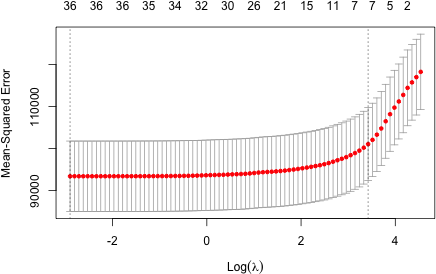
\includegraphics{Project_files/figure-latex/unnamed-chunk-41-1.png}

\begin{Shaded}
\begin{Highlighting}[]
\CommentTok{\# Select the lambda value that minimizes the mean}
\CommentTok{\# cross{-}validation error}
\NormalTok{best\_lambda }\OtherTok{\textless{}{-}}\NormalTok{ cv\_model}\SpecialCharTok{$}\NormalTok{lambda.min}

\CommentTok{\# Fit a Lasso regression model with the selected lambda}
\CommentTok{\# value}
\NormalTok{lasso\_model\_best }\OtherTok{\textless{}{-}} \FunctionTok{glmnet}\NormalTok{(x\_train, y\_train, }\AttributeTok{alpha =} \DecValTok{1}\NormalTok{, }\AttributeTok{lambda =}\NormalTok{ best\_lambda)}

\CommentTok{\# Calculate R{-}squared and multiple R{-}squared}
\NormalTok{y\_train\_pred }\OtherTok{\textless{}{-}} \FunctionTok{predict}\NormalTok{(lasso\_model\_best, }\AttributeTok{newx =}\NormalTok{ x\_train)}
\NormalTok{y\_train\_mean }\OtherTok{\textless{}{-}} \FunctionTok{mean}\NormalTok{(y\_train)}
\NormalTok{SST }\OtherTok{\textless{}{-}} \FunctionTok{sum}\NormalTok{((y\_train }\SpecialCharTok{{-}}\NormalTok{ y\_train\_mean)}\SpecialCharTok{\^{}}\DecValTok{2}\NormalTok{)}
\NormalTok{SSR }\OtherTok{\textless{}{-}} \FunctionTok{sum}\NormalTok{((y\_train }\SpecialCharTok{{-}}\NormalTok{ y\_train\_pred)}\SpecialCharTok{\^{}}\DecValTok{2}\NormalTok{)}
\NormalTok{R\_squared }\OtherTok{\textless{}{-}} \DecValTok{1} \SpecialCharTok{{-}}\NormalTok{ SSR}\SpecialCharTok{/}\NormalTok{SST}
\NormalTok{multiple\_R\_squared }\OtherTok{\textless{}{-}} \FunctionTok{cor}\NormalTok{(y\_train\_pred, y\_train)}\SpecialCharTok{\^{}}\DecValTok{2}
\NormalTok{n }\OtherTok{\textless{}{-}} \FunctionTok{length}\NormalTok{(y\_train)}
\NormalTok{p }\OtherTok{\textless{}{-}} \FunctionTok{ncol}\NormalTok{(x\_train)}
\NormalTok{adj\_R\_squared }\OtherTok{\textless{}{-}} \DecValTok{1} \SpecialCharTok{{-}}\NormalTok{ (SSR}\SpecialCharTok{/}\NormalTok{(n }\SpecialCharTok{{-}}\NormalTok{ p }\SpecialCharTok{{-}} \DecValTok{1}\NormalTok{))}\SpecialCharTok{/}\NormalTok{(SST}\SpecialCharTok{/}\NormalTok{(n }\SpecialCharTok{{-}} \DecValTok{1}\NormalTok{))}


\CommentTok{\# Print the R{-}squared and multiple R{-}squared values}
\FunctionTok{cat}\NormalTok{(}\StringTok{"R{-}squared:"}\NormalTok{, }\FunctionTok{round}\NormalTok{(R\_squared, }\DecValTok{3}\NormalTok{), }\StringTok{"}\SpecialCharTok{\textbackslash{}n}\StringTok{"}\NormalTok{)}
\end{Highlighting}
\end{Shaded}

\begin{verbatim}
## R-squared: 0.214
\end{verbatim}

\begin{Shaded}
\begin{Highlighting}[]
\FunctionTok{cat}\NormalTok{(}\StringTok{"Multiple R{-}squared:"}\NormalTok{, }\FunctionTok{round}\NormalTok{(multiple\_R\_squared, }\DecValTok{3}\NormalTok{), }\StringTok{"}\SpecialCharTok{\textbackslash{}n}\StringTok{"}\NormalTok{)}
\end{Highlighting}
\end{Shaded}

\begin{verbatim}
## Multiple R-squared: 0.214
\end{verbatim}

\begin{Shaded}
\begin{Highlighting}[]
\FunctionTok{cat}\NormalTok{(}\StringTok{"Adjusted R{-}squared:"}\NormalTok{, }\FunctionTok{round}\NormalTok{(adj\_R\_squared, }\DecValTok{3}\NormalTok{), }\StringTok{"}\SpecialCharTok{\textbackslash{}n}\StringTok{"}\NormalTok{)}
\end{Highlighting}
\end{Shaded}

\begin{verbatim}
## Adjusted R-squared: 0.213
\end{verbatim}

\begin{Shaded}
\begin{Highlighting}[]
\CommentTok{\# Predict on the test data}
\NormalTok{x\_test }\OtherTok{\textless{}{-}} \FunctionTok{model.matrix}\NormalTok{(realSum }\SpecialCharTok{\textasciitilde{}}\NormalTok{ room\_type }\SpecialCharTok{+}\NormalTok{ person\_capacity }\SpecialCharTok{+}
\NormalTok{    host\_is\_superhost }\SpecialCharTok{+}\NormalTok{ multi }\SpecialCharTok{+}\NormalTok{ biz }\SpecialCharTok{+}\NormalTok{ cleanliness\_rating }\SpecialCharTok{+}\NormalTok{ guest\_satisfaction\_overall }\SpecialCharTok{+}
\NormalTok{    bedrooms }\SpecialCharTok{+} \FunctionTok{poly}\NormalTok{(dist, }\DecValTok{2}\NormalTok{) }\SpecialCharTok{+} \FunctionTok{poly}\NormalTok{(metro\_dist, }\DecValTok{2}\NormalTok{) }\SpecialCharTok{+} \FunctionTok{poly}\NormalTok{(attr\_index\_norm,}
    \DecValTok{2}\NormalTok{) }\SpecialCharTok{+} \FunctionTok{poly}\NormalTok{(rest\_index\_norm, }\DecValTok{2}\NormalTok{) }\SpecialCharTok{+}\NormalTok{ lng }\SpecialCharTok{+}\NormalTok{ lat }\SpecialCharTok{+}\NormalTok{ city\_day, }\AttributeTok{data =}\NormalTok{ my\_data\_test)[,}
    \SpecialCharTok{{-}}\DecValTok{1}\NormalTok{]}
\NormalTok{y\_test }\OtherTok{\textless{}{-}}\NormalTok{ my\_data\_test}\SpecialCharTok{$}\NormalTok{realSum}
\NormalTok{lasso\_pred }\OtherTok{\textless{}{-}} \FunctionTok{predict}\NormalTok{(lasso\_model\_best, }\AttributeTok{newx =}\NormalTok{ x\_test)}

\CommentTok{\# Evaluate the model performance}
\NormalTok{rmse }\OtherTok{\textless{}{-}} \FunctionTok{sqrt}\NormalTok{(}\FunctionTok{mean}\NormalTok{((y\_test }\SpecialCharTok{{-}}\NormalTok{ lasso\_pred)}\SpecialCharTok{\^{}}\DecValTok{2}\NormalTok{))}
\CommentTok{\# Print the R{-}squared and multiple R{-}squared values}
\FunctionTok{cat}\NormalTok{(}\StringTok{"RMSE on test set:"}\NormalTok{, }\FunctionTok{round}\NormalTok{(rmse, }\DecValTok{3}\NormalTok{), }\StringTok{"}\SpecialCharTok{\textbackslash{}n}\StringTok{"}\NormalTok{)}
\end{Highlighting}
\end{Shaded}

\begin{verbatim}
## RMSE on test set: 235.35
\end{verbatim}

Even Lasso regression is not good because of extremely low value of
R\^{}2 even in polynominal model of power 2 and 3.

\hypertarget{conclusion-at-this-point-in-time}{%
\section{Conclusion at this Point in
Time}\label{conclusion-at-this-point-in-time}}

Even though EDA has given us good insights in price determinants, both
Linear and Lasso Step Regression are not good for this case which is to
be expected since all common data tends to be generally skewed Normal or
Guassian(to be tested).

Further modelling is required and will be conducted which includes
trying of different linear techniques and also models from different
family.

\end{document}
